%----------
%   IMPORTANTE
%----------
% Plantilla oficial UC3M (estilo IEEE) rellenada con el contenido real del TFG.
% Se conserva el preambulo oficial (pdflatex + pdfx PDF/A-1b + txfonts +
% biblatex-ieee/biber + titlesec + estilos de tabla/figura). Se anaden solo los
% paquetes que el contenido necesita, todos compatibles con pdflatex. Copia de
% seguridad del placeholder oficial en memoria_PLANTILLA_ORIGINAL.tex.

%----------
%	CONFIGURACION DEL DOCUMENTO
%----------
\documentclass[12pt]{report}

\usepackage[a4paper, vmargin=2.5cm, hmargin=3cm]{geometry}
\renewcommand{\baselinestretch}{1.15}
\parskip=6pt

\usepackage[table]{xcolor}
\definecolor{azulUC3M}{RGB}{0,0,102}
\definecolor{gray97}{gray}{.97}
\definecolor{gray75}{gray}{.75}
\definecolor{gray45}{gray}{.45}

% PDF/A para e-Archivo (metadatos en output.xmpdata)
\usepackage[a-1b]{pdfx}

\usepackage{hyperref}
\hypersetup{colorlinks=true, linkcolor=black, urlcolor=blue}

% MATEMATICAS
\usepackage{amsmath,amssymb,amsfonts,amsthm}
\usepackage{mathtools}
\usepackage{bm}

% Codificacion
\usepackage{txfonts}
\usepackage[T1]{fontenc}
\usepackage[utf8]{inputenc}

% Idioma
\usepackage[spanish, es-tabla]{babel}
\usepackage[babel, spanish=spanish]{csquotes}
\AtBeginEnvironment{quote}{\small}

% Pie de pagina
\usepackage{fancyhdr}
\pagestyle{fancy}
\fancyhf{}
\renewcommand{\headrulewidth}{0pt}
\rfoot{\thepage}
\fancypagestyle{plain}{\pagestyle{fancy}}

% Titulos (titlesec/titletoc)
\usepackage{titlesec}
\usepackage{titletoc}
\titleformat{\chapter}[block]
{\large\bfseries\filcenter}{\thechapter.}{5pt}{\MakeUppercase}{}
\titlespacing{\chapter}{0pt}{0pt}{*3}
\titlecontents{chapter}[0pt]{}
{\contentsmargin{0pt}\thecontentslabel.\enspace\uppercase}
{\contentsmargin{0pt}\uppercase}{\titlerule*[.7pc]{.}\contentspage}
\titleformat{\section}{\bfseries}{\thesection.}{5pt}{}
\titlecontents{section}[5pt]{}
{\contentsmargin{0pt}\thecontentslabel.\enspace}
{\contentsmargin{0pt}}{\titlerule*[.7pc]{.}\contentspage}
\titleformat{\subsection}{\normalsize\bfseries}{\thesubsection.}{5pt}{}
\titlecontents{subsection}[10pt]{}
{\contentsmargin{0pt}\thecontentslabel.\enspace}
{\contentsmargin{0pt}}{\titlerule*[.7pc]{.}\contentspage}

% TABLAS
\usepackage{multirow}
\usepackage{caption}
\usepackage{subcaption}
\usepackage{floatrow}
\usepackage{array}
\usepackage{booktabs}
\usepackage{tabularx}
\usepackage{longtable}
\usepackage{float}
\newcolumntype{P}[1]{>{\centering\arraybackslash}p{#1}}
\DeclareCaptionFormat{upper}{#1#2\uppercase{#3}\par}
\captionsetup*[table]{format=upper, name=TABLA, justification=centering,
	labelsep=period, width=.75\linewidth, labelfont=small, font=small}

% FIGURAS
\usepackage{graphicx}
\graphicspath{{imagenes/}{../memoria_latex/figures/}{../UCIrvine/figures/}}
\captionsetup[figure]{format=hang, name=Fig., singlelinecheck=off,
	labelsep=period, labelfont=small, font=small}

% LISTAS, SI, EURO, ALGORITMOS, TikZ
\usepackage{enumitem}
\usepackage{siunitx}
\sisetup{output-decimal-marker={,},group-separator={\,}}
\usepackage{eurosym}
\usepackage{algorithm}
\usepackage{algpseudocode}
\usepackage{tikz}
\usetikzlibrary{arrows.meta,positioning,shapes.geometric,calc,patterns}

% NOTAS AL PIE
\usepackage{chngcntr}
\counterwithout{footnote}{chapter}

% LISTADOS DE CODIGO
\usepackage{listings}
\lstdefinestyle{estilo}{ frame=Ltb, framerule=0pt, aboveskip=0.5cm,
	framextopmargin=3pt, framexbottommargin=3pt, framexleftmargin=0.4cm,
	framesep=0pt, rulesep=.4pt, backgroundcolor=\color{gray97},
	rulesepcolor=\color{black}, basicstyle=\ttfamily\footnotesize,
	keywordstyle=\bfseries, stringstyle=\ttfamily, showstringspaces=false,
	commentstyle=\color{gray45}, numbers=left, numbersep=15pt,
	numberstyle=\tiny, numberfirstline=false, breaklines=true,
	xleftmargin=\parindent}
\captionsetup*[lstlisting]{font=small, labelsep=period}
\lstset{style=estilo}
\renewcommand{\lstlistingname}{\uppercase{Código}}

% BIBLIOGRAFIA IEEE (biblatex + biber)
\usepackage[backend=biber, style=ieee, isbn=false,sortcites, maxbibnames=6, minbibnames=1]{biblatex}
\DefineBibliographyStrings{spanish}{%
	andothers = {et\addabbrvspace al\adddot}}
\DefineBibliographyStrings{spanish}{
	url = {\adddot\space[En línea]\adddot\space Disponible en:}}
\DefineBibliographyStrings{spanish}{urlseen = {Acceso:}}
\DefineBibliographyStrings{spanish}{pages = {pp\adddot}, page = {p.\adddot}}
\addbibresource{referencias.bib}

% \cref (cargar tras hyperref)
\usepackage[noabbrev,nameinlink,spanish]{cleveref}

% ACRONIMOS
\usepackage[acronym,nonumberlist,toc]{glossaries}
\makeglossaries
% ─────────────────────────────────────────────────────────────────────
%  Acrónimos del TFG
% ─────────────────────────────────────────────────────────────────────

\newacronym{ai}{IA}{Inteligencia Artificial (\textit{Artificial Intelligence})}
\newacronym{ami}{AMI}{Infraestructura de Medida Avanzada (\textit{Advanced Metering Infrastructure})}
\newacronym{ae}{AE}{Autoencoder}
\newacronym{auc}{AUC}{Área Bajo la Curva (\textit{Area Under the Curve})}
\newacronym{aucpr}{AUC-PR}{Área bajo la curva Precision–Recall}
\newacronym{aucroc}{AUC-ROC}{Área bajo la curva ROC}
\newacronym{cnn}{CNN}{Red Neuronal Convolucional (\textit{Convolutional Neural Network})}
\newacronym{cnpic}{CNPIC}{Centro Nacional de Protección de Infraestructuras y Ciberseguridad}
\newacronym{dl}{DL}{Aprendizaje Profundo (\textit{Deep Learning})}
\newacronym{dos}{DoS}{Denegación de Servicio (\textit{Denial of Service})}
\newacronym{edge}{Edge}{Computación en el Borde}
\newacronym{eda}{EDA}{Análisis Exploratorio de Datos (\textit{Exploratory Data Analysis})}
\newacronym{ffn}{FFN}{Red de Avance (\textit{Feed-Forward Network})}
\newacronym{fdi}{FDI}{Inyección de Datos Falsos (\textit{False Data Injection})}
\newacronym{fn}{FN}{Falso Negativo}
\newacronym{fp}{FP}{Falso Positivo}
\newacronym{gbdt}{GBDT}{Árboles Gradient Boosting (\textit{Gradient Boosted Decision Trees})}
\newacronym{gru}{GRU}{Unidad Recurrente con Compuertas (\textit{Gated Recurrent Unit})}
\newacronym{iec}{IEC}{Comisión Electrotécnica Internacional}
\newacronym{if}{IF}{Bosque de Aislamiento (\textit{Isolation Forest})}
\newacronym{incibe}{INCIBE}{Instituto Nacional de Ciberseguridad}
\newacronym{iot}{IoT}{Internet de las Cosas (\textit{Internet of Things})}
\newacronym{lopdgdd}{LOPDGDD}{Ley Orgánica de Protección de Datos y Garantía de Derechos Digitales}
\newacronym{lstm}{LSTM}{Memoria a Largo y Corto Plazo (\textit{Long Short-Term Memory})}
\newacronym{lgbm}{LightGBM}{\textit{Light Gradient Boosting Machine}}
\newacronym{mae}{MAE}{Error Absoluto Medio}
\newacronym{ml}{ML}{Aprendizaje Automático (\textit{Machine Learning})}
\newacronym{mlp}{MLP}{Perceptrón Multicapa (\textit{Multi-Layer Perceptron})}
\newacronym{mse}{MSE}{Error Cuadrático Medio}
\newacronym{nilm}{NILM}{Monitorización No Intrusiva de Cargas}
\newacronym{nis2}{NIS2}{Directiva (UE) 2022/2555 de Seguridad de Redes y Sistemas de Información}
\newacronym{nist}{NIST}{\textit{National Institute of Standards and Technology}}
\newacronym{ntl}{NTL}{Pérdidas No Técnicas (\textit{Non-Technical Losses})}
\newacronym{ocsvm}{OCSVM}{Máquina de Vectores Soporte de Una Clase}
\newacronym{rgpd}{RGPD}{Reglamento General de Protección de Datos (UE 2016/679)}
\newacronym{rnn}{RNN}{Red Neuronal Recurrente}
\newacronym{roc}{ROC}{Curva Característica Operativa del Receptor}
\newacronym{scada}{SCADA}{Supervisión, Control y Adquisición de Datos}
\newacronym{shap}{SHAP}{\textit{SHapley Additive exPlanations}}
\newacronym{tcn}{TCN}{Red Convolucional Temporal}
\newacronym{tn}{TN}{Verdadero Negativo}
\newacronym{tp}{TP}{Verdadero Positivo}
\newacronym{tfg}{TFG}{Trabajo Fin de Grado}
\newacronym{uci}{UCI}{Universidad de California, Irvine (Repositorio)}
\newacronym{ukdale}{UK-DALE}{\textit{UK Domestic Appliance-Level Electricity}}
\newacronym{xai}{XAI}{Inteligencia Artificial Explicable (\textit{Explainable AI})}
% ── Ampliación NB15-NB20 ──
\newacronym{vae}{VAE}{Autoencoder Variacional (\textit{Variational Autoencoder})}
\newacronym{elbo}{ELBO}{Cota Inferior de la Evidencia (\textit{Evidence Lower Bound})}
\newacronym{ddpm}{DDPM}{Modelo Probabilístico de Difusión con Eliminación de Ruido (\textit{Denoising Diffusion Probabilistic Model})}
\newacronym{fl}{FL}{Aprendizaje Federado (\textit{Federated Learning})}
\newacronym{fedavg}{FedAvg}{Promediado Federado (\textit{Federated Averaging})}
\newacronym{dp}{DP}{Privacidad Diferencial (\textit{Differential Privacy})}
\newacronym{dpsgd}{DP-SGD}{Descenso de Gradiente Estocástico con Privacidad Diferencial}
\newacronym{rdp}{RDP}{Privacidad Diferencial de Rényi (\textit{Rényi Differential Privacy})}
\newacronym{fgsm}{FGSM}{Método del Signo del Gradiente Rápido (\textit{Fast Gradient Sign Method})}
\newacronym{pgd}{PGD}{Descenso de Gradiente Proyectado (\textit{Projected Gradient Descent})}
\newacronym{cw}{C\&W}{Ataque de Carlini y Wagner}
\newacronym{ptq}{PTQ}{Cuantización Post-Entrenamiento (\textit{Post-Training Quantization})}
\newacronym{qat}{QAT}{Entrenamiento Consciente de la Cuantización (\textit{Quantization-Aware Training})}
\newacronym{ece}{ECE}{Error de Calibración Esperado (\textit{Expected Calibration Error})}
\newacronym{gnn}{GNN}{Red Neuronal de Grafos (\textit{Graph Neural Network})}


% TEOREMAS
\theoremstyle{remark}
\newtheorem{observacion}{Observación}[chapter]
\newtheorem{ejemplo}{Ejemplo}[chapter]
\newtheorem{definicion}{Definición}[chapter]

% COMANDOS PERSONALIZADOS
\newcommand{\vires}{\mathrm{VI}_{\text{res}}}
\newcommand{\aucpr}{\text{AUC-PR}}
\newcommand{\aucroc}{\text{AUC-ROC}}
\newcommand{\fone}{F_{1}}
\newcommand{\ftwo}{F_{2}}
\newcommand{\code}[1]{\texttt{\small #1}}

%-------------
%	DOCUMENTO
%-------------
\begin{document}
\pagenumbering{roman}

%----------
%	PORTADA
%----------
\begin{titlepage}
	\begin{sffamily}
	\color{azulUC3M}
	\begin{center}
		\begin{figure}[H]
			\makebox[\textwidth][c]{
\includegraphics[width=16cm]{logo_UC3M.png}}
		\end{figure}
		\vspace{2.5cm}
		\begin{Large}
			Grado en Ingeniería de Telecomunicación\\
			 2025-2026\\
			\vspace{2cm}
			\textsl{Trabajo Fin de Grado}
			\bigskip
		\end{Large}
		 	{\Huge Detección de ataques de inyección de datos falsos en contadores inteligentes mediante aprendizaje automático no supervisado}\\
		 	\vspace*{0.5cm}
	 		\rule{10.5cm}{0.1mm}\\
			\vspace*{0.9cm}
			{\LARGE Matvey Sinelnik}\\
			\vspace*{1cm}
		\begin{Large}
			Tutora\\
			Marta Moure Garrido\\
			Leganés, Madrid\\
		\end{Large}
	\end{center}
	\vfill
	\color{black}
	
\includegraphics[width=4.2cm]{creativecommons.png}\\
	Esta obra se encuentra sujeta a la licencia Creative Commons \textbf{Reconocimiento - No Comercial - Sin Obra Derivada}
	\end{sffamily}
\end{titlepage}

\newpage
\thispagestyle{empty}
\mbox{}

%----------
%	RESUMEN
%----------
\renewcommand\abstractname{\large\bfseries\filcenter\uppercase{Resumen}}
\begin{abstract}
\thispagestyle{plain}
\setcounter{page}{3}

	La red eléctrica que llega a nuestras casas ya no es la de hace veinte años. Hoy cada vivienda en España tiene un contador inteligente que reporta su consumo cada pocos minutos, y esa cadena de medida es la base sobre la que se calcula la factura y se planifica la demanda. El problema es evidente: si alguien manipula esos datos ---los llamados ataques de inyección de datos falsos o FDI (\textit{False Data Injection})--- el operador toma decisiones sobre información comprometida. Este Trabajo Fin de Grado se ocupa de detectar esa manipulación sin recurrir a etiquetas de ataque, partiendo del conjunto público \textit{UCI Individual Household Electric Power Consumption} (algo más de dos millones de registros minuto a minuto durante 47 meses).

	Como no existen datos públicos de ataques FDI reales sobre contadores domésticos, se construye un banco sintético de siete tipos de ataque, organizados en cuatro familias ---magnitud, temporal, patrón y físico--- con tres niveles de severidad. Los rangos se eligen por argumento económico: por debajo de un fraude del 15\,\% el ataque ya no resulta rentable, así que ataques más leves no son realistas. Sobre ese banco se entrenan y comparan ocho detectores con el mismo protocolo y el mismo particionado temporal: dos clásicos (\textit{Isolation Forest} y un híbrido con K\nobreakdash-Means), cuatro autoencoders profundos (denso, LSTM, convolucional y \textit{transformer}), un LightGBM supervisado como techo, y un \textit{stacking} sobre todos ellos. El trabajo también propone una característica con motivación física, $\vires$, que mide cuánto se aleja la potencia reportada de la que implica el producto $V\cdot I$; cuando el atacante manipula la primera pero no controla la corriente, esa invariante se rompe y resulta diagnóstica.

	El sistema incluye un postprocesado temporal por votación causal $W/K$, un análisis de explicabilidad con SHAP, una evaluación de transferencia al \textit{dataset} UK-DALE y un análisis de robustez frente a atacantes adaptativos. El mejor detector no supervisado obtiene un AUC-PR competitivo con una latencia mediana por debajo de los cinco minutos y un tamaño en disco de pocos centenares de kilobytes, lo bastante ligero para ejecutarse en el propio contador. Se cierra con un capítulo sobre el marco regulador europeo y español (RGPD, NIS2, Ley 8/2011 de protección de infraestructuras críticas) y un análisis socioeconómico del proyecto.

	\textbf{Palabras clave:} detección de anomalías; ataques de inyección de datos falsos; contadores inteligentes; aprendizaje profundo; \textit{autoencoder}; \textit{transformer}; ciberseguridad de redes eléctricas; \textit{edge computing}.

	\vfill
\end{abstract}
	\newpage
	\thispagestyle{empty}
	\mbox{}

%----------
%	ABSTRACT
%----------
\renewcommand\abstractname{\large\bfseries\filcenter\uppercase{Abstract}}
\begin{abstract}
\thispagestyle{plain}

	Every household in Spain now has a smart meter reporting consumption every few minutes. That data feeds billing systems and demand forecasts, so anyone tampering with it puts the operator on the back foot. False Data Injection (FDI) attacks are precisely that kind of tampering, and they are hard to spot because the manipulated readings still look plausible. This Bachelor's thesis tackles their unsupervised detection on residential electric consumption time series, using the public \textit{UCI Individual Household Electric Power Consumption} dataset (just over two million one-minute records across 47 months).

	Since no public dataset of real FDI attacks on domestic meters exists, we build a synthetic bench with seven attack types organised into four families ---magnitude, temporal, pattern and physical--- with three severity levels. The severity ranges are picked by an economic argument: below roughly a 15\,\% theft factor, the attack stops being profitable, so milder ones are unrealistic. On this bench we train and compare eight detectors under the same protocol and the same strict temporal split: two classical (\textit{Isolation Forest} and a K\nobreakdash-Means hybrid), four deep autoencoders (dense, LSTM, convolutional and transformer), a supervised LightGBM as a ceiling, and a stacking ensemble on top of all of them. We also introduce a physics-grounded feature, $\vires$, that measures how much the reported active power departs from the value implied by $V\cdot I$; when an attacker tampers with the power but cannot control the current, that invariant breaks and becomes diagnostic.

	The system adds a causal $W/K$ temporal voting post-processor, a SHAP explainability layer, a cross-domain transfer evaluation on UK-DALE, and an adaptive-attacker robustness study. The best unsupervised detector reaches a competitive AUC-PR with a median detection latency below five minutes and a model footprint of a few hundred kilobytes ---light enough to run on the meter itself. The thesis closes with the European and Spanish regulatory framework (GDPR, NIS2, Law 8/2011 on critical infrastructure protection) and a socio-economic analysis of the project.

	\textbf{Keywords:} anomaly detection; false data injection; smart meters; deep learning; \textit{autoencoder}; \textit{transformer}; smart-grid cybersecurity; edge computing.

	\vfill
\end{abstract}
	\newpage
	\thispagestyle{empty}
	\mbox{}

%----------
%	DEDICATORIA
%----------
\chapter*{Dedicatoria}
	\noindent A mi familia y a quienes me han acompañado durante el grado.
	\vfill
	\newpage
	\thispagestyle{empty}
	\mbox{}

%----------
%	INDICES
%----------
\tableofcontents
\thispagestyle{fancy}
\newpage
\thispagestyle{empty}
\mbox{}

\listoffigures
\thispagestyle{fancy}
\newpage
\thispagestyle{empty}
\mbox{}

\listoftables
\thispagestyle{fancy}
\newpage
\thispagestyle{empty}
\mbox{}

\printglossary[type=\acronymtype,title={Glosario de acrónimos},toctitle={Glosario de acrónimos}]
\thispagestyle{fancy}
\newpage
\thispagestyle{empty}
\mbox{}

%----------
%	MEMORIA
%----------
\clearpage
\pagenumbering{arabic}

% ─────────────────────────────────────────────────────────────────────
%  Capítulo 1 — Introducción
% ─────────────────────────────────────────────────────────────────────
\chapter{Introducción}
\label{cap:introduccion}

\section{Contexto y motivación}
\label{sec:contexto}

Pocas infraestructuras han cambiado tanto en una década como la red eléctrica. Los sensores distribuidos, las comunicaciones bidireccionales y, sobre todo, los contadores inteligentes han convertido lo que era una red analógica en una \textit{smart grid} que monitoriza el consumo cada pocos minutos y gestiona la demanda con información granular del usuario final \cite{fang2012smartgrid,gungor2011smartgrid}. La Directiva 2009/72/CE de la Unión Europea fijó el objetivo de que al menos el 80\,\% de los consumidores tuvieran contador inteligente en 2020; España lo hizo antes, con un parque de unos 28 millones de contadores ya operativo en 2018--2019 \cite{cnmc2019contadores}. Sobre esa capa de medida se han construido servicios que en la red del siglo XX eran impensables: tarifas dinámicas, agregación y respuesta a la demanda en tiempo real, integración del autoconsumo y los vehículos eléctricos, e incluso analítica de eficiencia a nivel de hogar.

El precio de esta digitalización es una superficie de ataque que antes no existía. La AMI (Infraestructura de Medida Avanzada) son hoy millones de nodos IoT con conectividad bidireccional, capacidad de cómputo limitada y un ciclo de vida que se mide en décadas \cite{mclaughlin2016cybersecurity}. La \cref{fig:ami-fdi} resume esa cadena de medida y el punto en el que un atacante puede inyectar lecturas falsas. Comprometer uno solo de esos nodos no es un problema local: cualquier alteración en las lecturas viaja aguas arriba hasta facturación, previsión de demanda y, en el escenario adverso, hasta el operador del sistema. Aquí entran los ataques de inyección de datos falsos, o FDI \cite{liu2009fdi}, que destacan por una propiedad incómoda: pueden mantenerse \emph{stealth} ---invisibles para los estimadores de estado tradicionales--- mientras alteran datos críticos.

A nivel doméstico, los motivos para montar un ataque FDI suelen reducirse a tres. El primero y más obvio es la \textbf{reducción fraudulenta de la factura}: el atacante manipula su contador para que reporte menos consumo del real, y el sobrecoste acaba reflejado en la tarifa del resto a través de las llamadas \emph{pérdidas no técnicas} (NTL). El segundo es la \textbf{ocultación de consumo asociado a actividades ilícitas}; el caso clásico es el cultivo doméstico de cannabis o las granjas de minado de criptomonedas, cuyas firmas de consumo son tan características que basta con reportarlas fielmente para delatarse \cite{messinis2018review}. El tercero, menos frecuente pero el más peligroso, sería una \textbf{manipulación coordinada a gran escala}: un atacante con acceso a una fracción significativa del parque podría distorsionar la previsión agregada de demanda y forzar despachos económicos subóptimos o, en el peor caso, comprometer la estabilidad de la red \cite{liu2017review}.

Las cifras del problema son grandes. La literatura cifra las pérdidas no técnicas globales en torno al 1--3\,\% de la energía distribuida en países desarrollados, llegando al 30--40\,\% en algunas economías emergentes, lo que se traduce en pérdidas anuales superiores a los $96\,000$ millones de dólares en todo el mundo \cite{viegas2017review,messinis2018review}. En España las distribuidoras estiman entre 7\,000 y 9\,000\,GWh anuales de NTL, con una traslación al consumidor final del orden de varios euros por factura. Es decir: el problema justifica de sobra invertir en detección automática, sobre todo si esa detección es barata de ejecutar y respeta la privacidad procesando el dato en el propio contador.

La detección FDI ha pasado por tres generaciones de técnicas. La primera, basada en estadística clásica y \emph{state estimation} con detectores chi-cuadrado, mostró su techo pronto: Liu, Reiter y Ning probaron en 2009 \cite{liu2009fdi} que un atacante que conoce la topología puede construir vectores de ataque indetectables para esos residuales. La segunda generación, en los años 2010, trajo el aprendizaje automático clásico (\textit{Isolation Forest} \cite{liu2008isolation}, \textit{One-Class SVM}, \textit{Local Outlier Factor}) y modelos de regresión para captar desviaciones contextuales \cite{zheng2018wide,messinis2018review}. La generación actual se apoya en aprendizaje profundo: redes recurrentes y, más recientemente, arquitecturas \textit{transformer} para series temporales \cite{vaswani2017attention,nie2023patchtst,wu2023timesnet,xu2022anomaly}.

¿Dónde está, entonces, el hueco que pretende llenar este trabajo? La literatura compara casi siempre dos o tres modelos sobre datasets propios y con métricas que no casan entre sí, lo que hace difícil comparar de verdad. A esto se suman tres ausencias recurrentes: muy pocos artículos prueban a sus detectores contra atacantes que conocen el sistema; la explicabilidad de las decisiones se trata poco, pese a ser una exigencia en infraestructura crítica; y el coste de ejecutar el detector en el \textit{edge}, ahí donde está el contador, suele quedar fuera del análisis. Este TFG aborda los cuatro frentes de forma conjunta.

\begin{figure}[H]
  \centering
  \begin{tikzpicture}[
      node distance=12mm and 14mm,
      every node/.style={font=\small},
      box/.style={draw, rounded corners=2pt, minimum height=11mm, minimum width=20mm, align=center, thick},
      home/.style={box, fill=blue!8},
      meter/.style={box, fill=green!10, minimum width=24mm},
      conc/.style={box, fill=orange!12},
      head/.style={box, fill=red!10, minimum width=24mm},
      arr/.style={-{Latex[length=2.2mm]}, thick},
      atk/.style={draw, fill=red!75!black, text=white, font=\footnotesize\bfseries,
                  rounded corners=2pt, minimum width=18mm, minimum height=6mm}
  ]
    \node[home]  (h1) {Vivienda};
    \node[meter, right=of h1] (m1) {Contador\\\footnotesize\textit{smart meter}};
    \node[conc, right=of m1]  (c1) {Concentrador\\\footnotesize PLC / GPRS};
    \node[head, right=of c1]  (op) {Operador\\\footnotesize SCADA / MDM};

    \draw[arr] (h1) -- node[above, font=\scriptsize] {$V, I, P$} (m1);
    \draw[arr] (m1) -- node[above, font=\scriptsize] {lecturas} (c1);
    \draw[arr] (c1) -- node[above, font=\scriptsize] {agregado} (op);

    \node[atk] (a1) at ($(m1)!.5!(c1) + (0,-12mm)$) {Ataque FDI};
    \draw[arr, red!70!black, dashed, very thick]
      (a1.north) -- ($(m1.south)!.5!(c1.south)$)
      node[midway, right, font=\scriptsize, red!70!black] {inyección};

    \node[font=\scriptsize, gray, align=center] at ($(op)+(0,-13mm)$)
      {Facturación · gestión de demanda\\ previsión · liquidación};
  \end{tikzpicture}
  \caption{Cadena de medida AMI y vector de ataque FDI a nivel de contador. El atacante manipula la lectura entre el contador y el concentrador; el operador opera sobre datos comprometidos.}
  \label{fig:ami-fdi}
\end{figure}

\section{Planteamiento del problema}
\label{sec:problema}

Formalmente, sea $\bm{x}_t \in \mathbb{R}^d$ el vector de medidas que reporta el contador en el instante $t$ (potencia activa, reactiva, tensión, intensidad y submedidores) e $y_t \in \{0,1\}$ la etiqueta de ataque ---con $y_t=1$ si la lectura $\bm{x}_t$ ha sido manipulada. El problema es estimar $\hat y_t = f(\bm{x}_{t-W+1}, \ldots, \bm{x}_t)$ usando sólo muestras limpias en entrenamiento; es decir, sin que la función $f$ vea pares $(\bm{x}_t, y_t)$ con $y_t=1$.

La dificultad no viene de una sola fuente sino de la combinación de varias. El comportamiento normal del consumo doméstico es ya muy variable de por sí: hay estacionalidad diaria con picos de mañana y noche, semanal entre laborables y fines de semana, y anual marcada por la climatización, todo ello salpicado de ruido y eventos legítimos como una visita o un electrodoméstico de gran potencia. Encima, los ataques pueden ser sutiles: un escalado al 5\,\% bien construido se confunde con la variabilidad natural y resulta indistinguible a simple vista. Tampoco ayuda la ausencia de etiquetas: no hay corpus públicos de FDI reales sobre contadores domésticos, lo que obliga a trabajar de forma no supervisada (o semi-supervisada como mucho). Y todavía falta la restricción de despliegue: el detector tiene que correr con latencia de minutos y caber en la memoria de un dispositivo \textit{edge} o un concentrador embebido, normalmente del orden de decenas o centenares de kB de modelo y milisegundos por muestra.

\section{Objetivos del trabajo}
\label{sec:objetivos}

\subsection*{Objetivo general}

\noindent\textbf{OG.} Diseñar, implementar y evaluar un sistema de detección no supervisada de ataques de inyección de datos falsos sobre series temporales de contador eléctrico residencial, viable para despliegue en el extremo de la red (\textit{edge computing}).

\subsection*{Objetivos específicos}

Este objetivo general se concreta en siete objetivos específicos, cada uno con un criterio de verificación claro que se retoma en las conclusiones:

\begin{enumerate}[label=\textbf{OE\arabic*.},leftmargin=*,topsep=2pt]
  \item Caracterizar el conjunto de datos UCI \emph{Individual Household Electric Power Consumption} mediante análisis exploratorio para extraer patrones temporales, calidad y estacionalidades relevantes.
  \item Diseñar un banco de ataques FDI sintéticos representativo, físicamente plausible y económicamente justificado, con \textit{ground truth} exacto.
  \item Implementar y comparar, bajo un protocolo de evaluación homogéneo, ocho detectores que cubran el espectro: clásicos (\textit{Isolation Forest}, K-Means+IF), profundos (autoencoders dense, LSTM, CNN, transformer), supervisado (LightGBM como techo), y un \textit{stacking} de los anteriores.
  \item Incorporar un postprocesado temporal por votación causal que reduzca la tasa de falsos positivos respetando la latencia de despliegue.
  \item Evaluar la explicabilidad de los detectores con mejor rendimiento mediante valores SHAP, identificando las características clave en la decisión.
  \item Estimar la generalización del sistema sobre un dominio distinto (UK-DALE) y la robustez frente a atacantes adaptativos que conocen el detector.
  \item Cuantificar la viabilidad de despliegue en el \textit{edge}: tamaño del modelo, latencia mediana y coste por muestra.
\end{enumerate}

\section{Metodología y enfoque}
\label{sec:metodologia}

El trabajo sigue una metodología experimental con ciclos cortos de diseño, implementación y evaluación. Se arrancó con un análisis exploratorio del dataset UCI, se diseñó e implementó el banco de ataques sintéticos, y a continuación se montaron, entrenaron y calibraron los ocho detectores. La evaluación combina una parte cuantitativa bajo protocolo homogéneo ---con énfasis en AUC-PR y en métricas operativas como latencia y tamaño--- y una parte cualitativa centrada en explicabilidad. Cierran el ciclo los análisis críticos de generalización, robustez frente a atacantes adaptativos y viabilidad de despliegue. La memoria y la defensa se redactan en la última fase.

Toda la implementación corre sobre Python 3.11, con TensorFlow 2.18 acelerado vía la API Metal de Apple Silicon (M2 Pro), scikit-learn 1.5 y LightGBM 4.5, encadenados en \textit{notebooks} Jupyter versionados con Git. Los resultados son reproducibles re-ejecutando cada notebook desde la primera celda con \code{nbconvert --execute}, fijando las semillas (test=42, validación=777). El repositorio mantiene la correspondencia uno a uno entre cada notebook numerado y la sección del \cref{cap:diseno} que lo describe.

\section{Estructura del documento}
\label{sec:estructura}

El resto del documento se organiza en ocho capítulos y un bloque de anexos. El \textbf{Cap.~\ref{cap:estado}} hace un repaso del estado del arte ---ciberseguridad de \textit{smart grids}, detección de anomalías energéticas, taxonomías FDI, explicabilidad y \textit{edge computing}--- y cierra explicitando la brecha que justifica el trabajo. El \textbf{Cap.~\ref{cap:teorico}} cubre los fundamentos teóricos: series temporales, modelos clásicos y profundos (autoencoders, CNN, LSTM, \textit{transformer}), \textit{boosting} y métricas. Los datos y el banco de ataques sintéticos se describen en el \textbf{Cap.~\ref{cap:datos}}, que incluye también el análisis exploratorio, el particionado temporal y la ingeniería de características. El \textbf{Cap.~\ref{cap:diseno}} detalla, para cada uno de los ocho detectores, la arquitectura, el entrenamiento, la calibración del umbral y el postprocesado temporal; sus resultados ---por tipo y severidad de ataque, con SHAP, transferencia a UK-DALE y robustez adversaria--- se discuten en el \textbf{Cap.~\ref{cap:resultados}}. El \textbf{Cap.~\ref{cap:conclusiones}} retoma los objetivos del Cap.~\ref{cap:introduccion} uno a uno para verificar su cumplimiento, reconoce limitaciones y propone líneas futuras. El \textbf{Cap.~\ref{cap:regulador}} cubre el marco regulador (RGPD, NIS2, Ley 8/2011, IEC 62351) y el entorno socioeconómico (presupuesto, planificación e impacto). Los anexos recogen los detalles de implementación, las tablas extendidas y todo lo necesario para reproducir el trabajo.

\noindent Por convención, la memoria usa la primera persona del plural de modestia (\textit{``se ha implementado''}, \textit{``hemos calibrado''}) y mantiene en cursiva los términos técnicos en inglés (\textit{autoencoder}, \textit{stacking}, \textit{transformer}, \textit{edge}, \textit{dataset}\ldots) salvo aquellos ya plenamente asentados en el castellano técnico.

% ─────────────────────────────────────────────────────────────────────
%  Capítulo 2 — Estado del arte
% ─────────────────────────────────────────────────────────────────────
\chapter{Estado del arte}
\label{cap:estado}

Este capítulo recorre la literatura que da contexto al trabajo, agrupada en cinco bloques: ciberseguridad de las redes eléctricas inteligentes (\cref{sec:soa-cyber}), detección de anomalías en consumo eléctrico (\cref{sec:soa-ad}), simulación y taxonomías de ataques FDI (\cref{sec:soa-fdi}), explicabilidad y despliegue en el \textit{edge} (\cref{sec:soa-xai-edge}) y, ya como cierre, el posicionamiento del TFG frente a lo publicado (\cref{sec:soa-brecha}). La intención no es enumerar artículos uno detrás de otro, sino construir un argumento que justifique para qué sirve este trabajo.

\section{Ciberseguridad en redes eléctricas inteligentes}
\label{sec:soa-cyber}

Que la red eléctrica se haya convertido en un sistema ciberfísico ha generado una literatura abundante sobre amenazas y contramedidas. Una de las referencias más citadas es el trabajo de Mo \emph{et al.} \cite{mo2012cyberphysical}, que organiza el panorama según la clásica triada CIA aplicada al dominio eléctrico. Por el lado de la \textbf{confidencialidad}, el dato de consumo es información personal sensible: revela presencia, uso de electrodomésticos y patrones laborales, y existen técnicas bien documentadas para re-identificar usuarios a partir de su serie temporal \cite{molina2010private}. La \textbf{integridad} es el flanco donde encajan los ataques FDI, los más estudiados desde el clásico de Liu \emph{et al.} \cite{liu2009fdi}: un atacante con acceso a la matriz Jacobiana del estimador de estado puede construir vectores de ataque que pasan inadvertidos para los detectores chi-cuadrado basados en residuales. La \textbf{disponibilidad}, finalmente, cubre todo el repertorio clásico ---DoS sobre canales de comunicación, \textit{jamming} de PLC o WiFi, agotamiento de batería en contadores remotos--- recogido en revisiones como la de McLaughlin \emph{et al.} \cite{mclaughlin2016cybersecurity}.

Revisiones más recientes y específicas del plano de medida \cite{mehrdad2018cybersecurity,liang2017review} reagrupan los FDI domésticos en tres subclases con relevancia operativa: \emph{ataques de pillaje} (recortar selectivamente las lecturas), \emph{ataques de duplicación} (clonar las lecturas de otros usuarios) y \emph{ataques físicos} sobre el hardware del propio contador. Conviene separar dos problemas que a veces se confunden: el FDI a nivel de transporte se ataca con modelos del estimador de estado, pero a nivel residencial ese estimador no existe ---no hay observabilidad suficiente---, así que la única vía es el análisis estadístico y de patrones de la serie temporal. Ese es exactamente el terreno en el que se mueve este TFG.

Conviene detenerse en el concepto de \textbf{sistema ciberfísico}, porque está detrás de una de las decisiones de diseño más importantes del trabajo. El plano físico (potencia, tensión, corriente) y el plano cibernético (las medidas que llegan al operador) están acoplados por las leyes de la electricidad: la potencia activa reportada y la implícita por $V\cdot I$ deben coincidir, salvo pequeñas pérdidas resistivas. Si el atacante manipula la potencia pero no controla la corriente, esa invariante se rompe \cite{ahmad2025aif}. Sobre esta idea construimos la \textit{feature} $\vires$, una traslación al ámbito doméstico de la explotación de invariantes físicas que Pan \emph{et al.} \cite{pan2015fdi} ya ensayaron a nivel de transporte.

\section{Detección de anomalías en consumo eléctrico}
\label{sec:soa-ad}

La detección de anomalías en consumo eléctrico es un campo amplio, que abarca desde la detección de fallos en equipamiento hasta la detección de fraude. La revisión sistemática de Himeur \emph{et al.} \cite{himeur2021review} es una de las más completas y recientes, y organiza la literatura según paradigma de aprendizaje, nivel de detección, plataforma de cómputo y tratamiento de la privacidad. Leyéndola de forma crítica, los métodos se acaban agrupando en cuatro grandes familias.

\subsection{Métodos estadísticos y basados en reglas}

Son la base histórica del campo y siguen presentes en producción por su simplicidad e interpretabilidad. Caben aquí el control estadístico de procesos (\textit{control charts}, CUSUM, EWMA), los modelos ARIMA y SARIMA \cite{deboeck2007arima} y los umbrales fijos sobre características derivadas. La ventaja es evidente: no necesitan entrenamiento intensivo, no exigen etiquetas y son fáciles de auditar. La contrapartida también lo es: no capturan patrones temporales complejos ni interacciones entre variables. Hudani \emph{et al.} \cite{hudani2023realtime} demuestran que un sistema híbrido entre reglas y aprendizaje en línea puede operar en tiempo real con baja latencia, pero a costa de un \emph{tuning} cuidadoso por dominio.

\subsection{Aprendizaje automático clásico}

El salto cualitativo llega con el aprendizaje no supervisado clásico. El \textit{Isolation Forest}, propuesto por Liu \emph{et al.} \cite{liu2008isolation,liu2012iforest}, parte de una idea sencilla: las muestras anómalas, al ser raras y distintas, se aíslan con menos particiones aleatorias que las normales. Tiene pocos hiperparámetros, es paralelizable y resulta extraordinariamente rápido, lo que explica su popularidad como \textit{baseline}. Junto a él aparecen alternativas con propiedades complementarias: \textit{Local Outlier Factor} \cite{breunig2000lof}, que compara la densidad local de un punto con la de sus vecinos, y \textit{One-Class SVM} \cite{scholkopf2001ocsvm}, que aprende una frontera no lineal alrededor del conjunto normal usando núcleos.

El \textit{clustering} también ha jugado un papel doble en el campo: puede usarse de forma directa ---los puntos lejanos al centroide más próximo son sospechosos--- o como pre-procesado para entrenar detectores especializados por régimen, idea que recuperamos en nuestro detector híbrido K-Means+IF (NB03b). Vale la pena señalar el trabajo de Saglam \cite{saglam2023ml}, que compara cuatro detectores clásicos sobre series de consumo y concluye que el rendimiento depende casi por completo del preprocesado y de la calibración del umbral; nuestros experimentos confirman esa observación.

\subsection{Aprendizaje profundo}

Los \textit{autoencoders} son hoy el caballo de batalla de la detección no supervisada. La idea, que se remonta a Hinton y Salakhutdinov \cite{hinton2006reducing}, es sencilla: se entrena una red a reconstruir su propia entrada pasándola por un cuello de botella estrecho; lo que sale mal reconstruido es candidato a anomalía. Aplicado al consumo eléctrico, el paradigma ha generado un volumen creciente de propuestas, que conviene desglosar por arquitectura.

\paragraph{Autoencoders densos.} Castangia \emph{et al.} \cite{castangia2022density} aplican un AE denso al propio dataset UCI con resultados competitivos sin recurrir a etiquetas. Una variante interesante es la de Pereira y Silveira \cite{pereira2018unsupervised}, que usa autoencoders variacionales (VAE) para acompañar la detección con una medida de incertidumbre, algo especialmente útil cuando la alarma va a un operador humano.

\paragraph{Autoencoders recurrentes.} Las LSTM \cite{hochreiter1997lstm} ---y sus AE asociados--- encajan bien con las series temporales porque están pensadas para modelar dependencias largas. Malhotra \emph{et al.} \cite{malhotra2016lstmae} fueron quienes popularizaron el LSTM-AE para detección de anomalías, y trabajos posteriores como los de Pal \emph{et al.} \cite{pal2023lstm} o Mehedi \emph{et al.} \cite{mehedi2024gruae} confirman su utilidad tanto en consumo residencial como industrial.

\paragraph{Autoencoders convolucionales.} La convolución 1D aporta un sesgo inductivo temporal ---detecta patrones locales y es invariante a traslación--- con un coste de cómputo inferior al de la recurrencia. Un exponente clásico es \textit{DeepAnT} \cite{munir2018deepant}, una arquitectura convolucional que pronostica el siguiente valor y detecta anomalías por residual.

\paragraph{Transformers para series temporales.} Aquí está la frontera actual del campo. El \textit{transformer} de Vaswani \emph{et al.} \cite{vaswani2017attention}, que arrasó en PLN en 2017, ha tardado más en aterrizar en series temporales porque la atención cuadrática es cara para secuencias largas. Sucesivas propuestas han ido buscando alternativas viables: \textit{Informer} \cite{zhou2021informer}, \textit{Autoformer} \cite{wu2021autoformer}, \textit{Anomaly Transformer} \cite{xu2022anomaly}, \textit{PatchTST} \cite{nie2023patchtst}, \textit{TimesNet} \cite{wu2023timesnet} e \textit{iTransformer} \cite{liu2024itransformer}. PatchTST merece mención aparte: su idea es trocear la serie en \textit{patches} y tratarlos como \textit{tokens}, lo que reduce drásticamente el coste y captura mejor las dependencias locales. Es la idea de \textit{patching} la que adoptamos en nuestro detector basado en \textit{transformer} (NB08).

\subsection{Detección de fraude (NTL) y trabajos aplicados a contadores}

Existe un subcampo específico, el de las \emph{pérdidas no técnicas} (NTL) y el robo de electricidad, que es metodológicamente distinto al nuestro por una razón principal: ahí sí suele haber etiquetas. La fuente más usada son los datasets de la \textit{State Grid Corporation of China}, publicados en sucesivos \textit{challenges} y reutilizados ampliamente desde entonces \cite{zheng2018wide}. Buzau \emph{et al.} \cite{buzau2020hybrid} son un buen ejemplo: combinan mediciones y datos sociodemográficos para enriquecer la señal. La diferencia clave con nuestro problema no está en el método sino en el horizonte: el NTL se evalúa a nivel de \emph{cliente} ---¿este cliente es fraudulento?---, mientras que nosotros respondemos a nivel de \emph{minuto} ---¿este minuto contiene un ataque?---, lo que cambia tanto las métricas como los modelos.

\begin{table}[H]
\centering
\caption{Comparación esquemática de trabajos previos sobre detección de anomalías en consumo eléctrico y series temporales relacionadas. Ordenados cronológicamente.}
\label{tab:soa}
\footnotesize
\begin{tabularx}{\textwidth}{l X l l l}
\toprule
Ref. & Dataset & Tipo & Método & Métrica reportada \\
\midrule
Liu 2008 \cite{liu2008isolation}              & Sintético + KDD       & \textit{Outlier} puntual    & \textit{Isolation Forest}          & AUC-ROC 0{,}93--0{,}98 \\
Malhotra 2016 \cite{malhotra2016lstmae}       & Power demand          & Anomalía colectiva          & LSTM-AE                            & $\fone$ 0{,}81 \\
Jokar 2016 \cite{jokar2016electricity}        & Irlanda CER trial     & Robo electricidad           & SVM + reglas                       & TPR 0{,}94 / FPR 0{,}11 \\
Pereira 2018 (VAE) \cite{pereira2018unsupervised} & Solar PV power     & Residencial                 & Variational AE                     & $\fone$ 0{,}79 + incertidumbre \\
Munir 2018 (DeepAnT) \cite{munir2018deepant}  & NAB benchmark         & Contextual                  & CNN + residual                     & Precision 0{,}88 / Recall 0{,}77 \\
Buzau 2020 \cite{buzau2020hybrid}             & Endesa NTL            & Fraude                      & XGBoost + ANN                      & ROC-AUC 0{,}95 \\
Castangia 2022 \cite{castangia2022density}    & UCI Power             & Hogar                       & AE denso                           & $\fone$ $\sim$0{,}86 \\
Xu 2022 (Anomaly Tr.) \cite{xu2022anomaly}    & MSL, SMD, SWaT        & Multivariante               & Transformer + assoc.\ disc.        & $\fone$ 0{,}92--0{,}95 \\
Nie 2023 (PatchTST) \cite{nie2023patchtst}    & ETT, Electricity      & \textit{Forecast} / AD      & Transformer \emph{patched}         & MSE / $\fone$ SOTA \\
Saglam 2023 \cite{saglam2023ml}               & Consumo eléctrico ind.& Industrial                  & IF / OCSVM / LOF comparados        & $\fone$ 0{,}71--0{,}83 \\
Mehedi 2024 \cite{mehedi2024gruae}            & UCI + propio          & Hogar / FDI                 & GRU-AE                             & $\fone$ 0{,}88 \\
Ahmad 2025 (AIF) \cite{ahmad2025aif}          & Sintético AMI         & FDI                         & AE + MLP + invariantes físicas     & $\fone$ 0{,}92 \\
\midrule
\multicolumn{5}{l}{\footnotesize\textbf{Este TFG}: UCI Power + 7 ataques FDI sintéticos · 8 detectores comparados · $\fone$ 0{,}82 (no superv.) / 0{,}91 (techo)} \\
\bottomrule
\end{tabularx}
\end{table}

\section{Ataques FDI: taxonomías y simulación}
\label{sec:soa-fdi}

Al no haber datasets públicos con FDI reales etiquetados sobre contadores domésticos, la práctica habitual ---y aceptable, siempre que los ataques sean plausibles y estén bien documentados--- es simularlos sobre datos limpios. La literatura ofrece al menos tres taxonomías complementarias, según se mire el mecanismo de manipulación, el objetivo del atacante o sus capacidades. Por mecanismo aparecen el escalado multiplicativo, el desplazamiento aditivo, la inyección de ruido, la manipulación temporal (\textit{ramp}, \textit{step}) o la repetición de tramos históricos (\textit{replay}) \cite{jokar2016electricity,buzau2018detection}. Por objetivo, reducción de factura, ocultación de actividad ilícita o sabotaje de infraestructura \cite{messinis2018review}. Y por capacidad, atacantes oportunistas (sin modelo del detector), informados o adaptativos con acceso \textit{black-box} \cite{shokri2017membership,kos2018adversarial}.

Este TFG combina las dos primeras al agrupar sus siete tipos de ataque en cuatro categorías mecánicas (magnitud, temporal, patrón, físico) con tres niveles de severidad calibrados por argumento económico. La tercera ---la taxonomía por capacidad--- aparece más adelante, en el \cref{sec:resultados-adversarial}, para evaluar la robustez frente a atacantes que conocen el detector.

Hay un punto adicional sobre el que conviene insistir: la \emph{plausibilidad} del banco de ataques no es un detalle cosmético. Cuando los ataques simulados son demasiado burdos, los detectores rinden muy bien sobre el papel pero ese rendimiento no se sostiene en producción. Por eso, en el \cref{cap:datos} dedicamos espacio a justificar los rangos de severidad desde la rentabilidad económica del fraude: un atacante racional no se arriesga a una detección por un ahorro marginal del 5\,\%; el rango realmente rentable, según la literatura sobre sectores fraudulentos, está entre el 15 y el 50\,\% \cite{messinis2018review}.

\section{Explicabilidad y despliegue en el edge}
\label{sec:soa-xai-edge}

\subsection{Explicabilidad (XAI) en detección energética}

La inteligencia artificial explicable (XAI) ha dejado de ser un campo de nicho para convertirse en un requisito regulatorio. En infraestructura crítica esto va más allá del lujo: un operador no actúa sobre una alarma si no sabe por qué se ha disparado. La pieza central del marco es SHAP (\textit{SHapley Additive exPlanations}), que Lundberg y Lee \cite{lundberg2017shap} formalizaron sobre los valores de Shapley de la teoría de juegos cooperativos, dotando a las atribuciones de propiedades teóricas deseables como la eficiencia, la simetría o la aditividad. La aplicación práctica se ve facilitada por \textit{TreeExplainer} \cite{lundberg2020fromlocal}, que calcula los SHAP exactos en árboles (LightGBM, XGBoost) en tiempo polinómico, lo que los hace operativamente viables.

En el ámbito de la detección de anomalías, Mahbooba \emph{et al.} \cite{mahbooba2021xai} aplican LIME y SHAP a modelos de detección de intrusión, y Tang \emph{et al.} \cite{tang2024xaienergy} llevan SHAP al contexto energético con detectores de anomalías de consumo. Nuestro enfoque sigue una línea parecida: aplicamos SHAP al detector supervisado (LightGBM) y al mejor autoencoder, y contrastamos las explicaciones con la intuición física. Que SHAP señale a $\vires$ como característica clave en los ataques de manipulación de tensión es, en ese sentido, una validación cruzada tanto del modelo como del propio banco de ataques.

\subsection{Edge computing para AMI}

Llevar la inteligencia al borde de la red ---el llamado \textit{edge}--- es uno de los pilares de la \textit{smart grid} actual \cite{shi2016edge,oliveira2021edge}. Las razones para hacerlo se acumulan: el dato sensible no sale del contador (privacidad), la latencia se reduce porque desaparece el viaje a la nube, el sistema se vuelve más resiliente ante caídas de comunicaciones y, al final, el centro de datos se descarga. Ahora bien, los contadores y concentradores son dispositivos pequeños: décimas o unidades de MB de memoria, CPUs ARM de bajo consumo y, casi siempre, sin GPU. Un modelo de cientos de MB no entra; uno de decenas o pocos centenares de kB sí.

Para conseguir modelos de \textit{deep learning} compatibles con esas restricciones, la receta habitual combina tres ingredientes: arquitecturas ligeras con pocos parámetros, cuantización a 8 o 4 bits y \textit{pruning} estructurado. TinyAnomaly \cite{nguyen2023tiny} es un buen ejemplo: detección de anomalías por debajo de 100 kB sobre microcontroladores ARM Cortex-M. La estrategia que seguimos en este TFG es ligeramente distinta: en lugar de comprimir a posteriori, diseñamos los modelos para que ya nazcan pequeños (Dense-AE $\sim$130 kB, CNN-AE $\sim$200 kB, LSTM-AE $\sim$740 kB), de modo que la viabilidad de despliegue es inmediata.

\section{Fronteras recientes: modelos generativos, aprendizaje distribuido y robustez}
\label{sec:soa-fronteras}

El estado del arte 2023--2025 ha desplazado el foco desde \emph{qué arquitectura reconstruye mejor} hacia cuatro ejes que un detector desplegable en infraestructura crítica no puede ignorar: la cuantificación de la incertidumbre, la síntesis generativa de datos, la privacidad del entrenamiento distribuido y la robustez frente a atacantes informados. Estos cuatro frentes vertebran la ampliación de este trabajo (\cref{sec:resultados-ampliacion}).

\subsection{Modelos generativos: del autoencoder variacional a la difusión}

El \textbf{autoencoder variacional} (VAE) de Kingma y Welling \cite{kingma2014vae} introduce un cuello de botella \emph{probabilístico}: en lugar de un punto latente, el codificador produce una distribución, lo que permite muestrear y, sobre todo, estimar la incertidumbre de cada reconstrucción. An y Cho \cite{an2015reconstruction} formalizan la \emph{probabilidad de reconstrucción} como \textit{score} de anomalía, que dota a cada alarma de una banda de confianza ---justo lo que Pereira y Silveira \cite{pereira2018unsupervised} ya señalaban como deseable para el operador humano---. El \textit{$\beta$-VAE} \cite{higgins2017betavae} regula el peso del término de divergencia para controlar la estructura del espacio latente.

Un paso más allá están los \textbf{modelos de difusión} (DDPM, Ho \emph{et al.} \cite{ho2020ddpm}), que aprenden a invertir un proceso de ruido gaussiano gradual y se han convertido en el estado del arte generativo. En series temporales destacan \textit{TimeGrad} \cite{rasul2021timegrad} y \textit{CSDI} \cite{tashiro2021csdi}, que generan trazas realistas condicionadas; y como detectores, \textit{AnoDDPM} \cite{wyatt2022anoddpm} explota el error de \emph{denoising} parcial para señalar anomalías. Su relevancia para este trabajo es doble: permiten sintetizar ataques sobre portadoras de consumo \emph{generadas} ---no copiadas de los datos--- y ofrecen una familia de detección alternativa a la reconstrucción.

\subsection{Aprendizaje federado y privacidad diferencial}

Centralizar las series de consumo de millones de hogares es indeseable (privacidad) e inviable (ancho de banda). El \textbf{\textit{federated learning}} (FedAvg, McMahan \emph{et al.} \cite{mcmahan2017fedavg}) entrena un modelo compartido intercambiando solo \emph{pesos}, nunca datos crudos; su aplicación a la \textit{smart grid} está revisada en Briggs \emph{et al.} \cite{briggs2020federated} y Li \emph{et al.} \cite{li2021federated}. Como los pesos pueden filtrar información (ataques de inferencia de pertenencia, Shokri \emph{et al.} \cite{shokri2017membership}), se combina con \textbf{privacidad diferencial}: el marco formal de Dwork y Roth \cite{dwork2014dp} y su instanciación práctica \textbf{DP-SGD} \cite{abadi2016dpsgd}, que recorta y ruidifica los gradientes. La contabilidad ajustada del presupuesto $\varepsilon$ se realiza hoy mediante \emph{Rényi Differential Privacy} \cite{mironov2017rdp} y su extensión al mecanismo gaussiano submuestreado \cite{mironov2019sgm}. Este eje conecta directamente con el marco regulador del \cref{cap:regulador}.

\subsection{Robustez adversaria frente a atacantes de gradiente}

La taxonomía por capacidad del \cref{sec:soa-fdi} culmina en el atacante de \emph{caja blanca} que conoce el detector. Frente a él, la búsqueda en rejilla es una amenaza débil: el estándar son los ataques basados en gradiente ---FGSM \cite{goodfellow2014fgsm}, PGD \cite{madry2018pgd} y la optimización con penalización $\ell_2$ de Carlini y Wagner \cite{carlini2017cw}---, ya ensayados sobre detectores energéticos por Chen \emph{et al.} \cite{chen2018adversarial} y Kos \emph{et al.} \cite{kos2018adversarial}. La defensa de referencia es el \emph{adversarial training} \cite{madry2018pgd}, y un argumento recurrente es que los \emph{ensembles} encarecen la evasión al exigir transferir el ataque entre modelos de gradientes distintos.

\subsection{Compresión de modelos para el edge}

Más allá de diseñar redes pequeñas, la receta madura combina \textbf{cuantización} a 8/4 bits \cite{jacob2018quantization} y \textbf{\textit{pruning}} con compresión \cite{han2016deepcompression}, que reducen el \textit{footprint} varios factores con pérdida marginal de precisión. Esto convierte la promesa \emph{edge-viable} en una medida cuantificable de tamaño, latencia y energía, evaluable incluso sobre TFLite-Micro en microcontroladores \cite{nguyen2023tiny}.

\section{Posicionamiento del trabajo y brecha identificada}
\label{sec:soa-brecha}

Releyendo la literatura con la pregunta de qué falta por hacer, aparecen cinco huecos concretos que este TFG intenta cubrir. El primero es metodológico: la mayoría de los trabajos comparan dos o tres modelos sobre datasets propios y métricas que no casan, lo que dificulta extraer conclusiones generales; aquí ponemos ocho detectores ---del \textit{Isolation Forest} a un \textit{transformer}--- a pelear sobre el mismo dataset, el mismo banco de ataques y el mismo protocolo. El segundo es la robustez frente a atacantes adaptativos: salvo excepciones como Chen \emph{et al.} \cite{chen2018adversarial}, la literatura asume atacantes oportunistas, mientras que nosotros evaluamos qué pasa cuando el atacante conoce el detector y se calibra a la frontera de detección.

A esto se añaden tres ejes que suelen quedar fuera. La explicabilidad operativa, donde SHAP no se usa solo para visualizar bonito sino para comprobar que las características clave del modelo coinciden con las que la física del problema señalaría. La generalización a otro dominio, que evaluamos sobre UK-DALE midiendo (sin maquillar) la caída de rendimiento. Y la viabilidad de despliegue en el \textit{edge}, que reportamos junto al AUC-PR con tamaño, latencia y coste por muestra, de manera que la elección de qué desplegar deja de ser una decisión de un solo número.

Esta combinación ---comparación amplia, robustez adversaria, explicabilidad, generalización y \textit{edge}--- no es habitual en la literatura, y es lo que constituye la aportación principal del trabajo.

% ─────────────────────────────────────────────────────────────────────
%  Capítulo 3 — Marco teórico
% ─────────────────────────────────────────────────────────────────────
\chapter{Marco teórico}
\label{cap:teorico}

Este capítulo agrupa los fundamentos teóricos sobre los que se apoyan los detectores y métricas de los capítulos siguientes. Damos por supuesto que el lector tiene la formación habitual de un ingeniero de telecomunicación ---señales y sistemas, estadística, álgebra lineal---, pero no asumimos base previa en \textit{deep learning}: por eso desarrollamos los modelos desde el perceptrón hasta el \textit{transformer}, sin atajos.

\section{Series temporales y detección de anomalías}
\label{sec:teo-ts}

Una \emph{serie temporal} es una sucesión de observaciones $\{x_t\}_{t=1}^{T}$ indexada por el tiempo, con $x_t \in \mathbb{R}^d$ en el caso multivariante. Una serie de consumo doméstico es típicamente multivariante (potencia activa, reactiva, tensión, intensidad, submedidores) y muestreada de forma uniforme (resolución de un minuto en el caso de UCI).

\begin{definicion}[Estacionariedad débil]
Una serie es \emph{débilmente estacionaria} si su media $\mu_t = \mathbb{E}[x_t]$ y su autocovarianza $\gamma(s, t) = \mathrm{Cov}(x_s, x_t)$ dependen solo del retardo $|s-t|$.
\end{definicion}

El consumo doméstico claramente no lo es: hay tendencias estacionales entre verano e invierno y patrones diarios y semanales evidentes. Existen técnicas clásicas para aislar tendencia, estacionalidad y residuo, como la descomposición STL \cite{cleveland1990stl}, pero aquí preferimos no aplicar descomposición explícita y dejar que sean los propios modelos ---sobre todo los recurrentes y los \textit{transformer}--- los que aprendan esa estructura desde los datos.

\subsection{Tipos de anomalía en series temporales}

La taxonomía clásica de Chandola \emph{et al.} \cite{chandola2009ad} distingue tres tipos de anomalía que se trasladan bien al caso de series temporales. Una anomalía \textbf{puntual} es una muestra suelta fuera del rango esperado ---un valor extremo aislado. Una anomalía \textbf{contextual} es un valor normal por sí solo pero raro en su contexto temporal, como un pico de consumo a las 3 de la mañana en un perfil habitualmente bajo a esa hora. Una anomalía \textbf{colectiva}, por último, es una sucesión de muestras que individualmente podrían pasar por normales pero que juntas forman un patrón inusual; los ataques FDI sostenidos en el tiempo ---\textit{ramp}, \textit{step}, \textit{replay}--- caen casi siempre en esta categoría, normalmente con un componente contextual añadido.

\subsection{Detección por reconstrucción}

En detección no supervisada sobre series temporales, el paradigma de referencia es la \emph{detección por reconstrucción}. La idea es directa: se entrena un modelo $f_\theta$ a reproducir con bajo error las muestras del conjunto limpio; lo que no reconstruye bien queda marcado como sospechoso. Formalmente, dado el detector con función de \emph{score}
\begin{equation}
s_\theta(\bm{x}) \;=\; \| \bm{x} - f_\theta(\bm{x}) \|_2^2,
\label{eq:rec-score}
\end{equation}
y un umbral $\tau$ calibrado sobre un conjunto de validación, la predicción es $\hat y_t = \mathbb{1}\{s_\theta(\bm{x}_t) > \tau\}$. La elección de $\tau$ y la posible ponderación por característica de la \cref{eq:rec-score} son decisiones de calibración clave que se desarrollan en \cref{cap:diseno}.

\section{Modelos clásicos de detección de anomalías}
\label{sec:teo-clasicos}

\subsection{Isolation Forest}

El \textit{Isolation Forest} \cite{liu2008isolation,liu2012iforest} parte de una intuición que resulta sorprendentemente eficaz: como las muestras anómalas son raras y diferentes, hacen falta menos particiones aleatorias para aislarlas que las normales. El algoritmo construye un bosque de árboles binarios aleatorios; en cada nodo elige al azar una característica y un umbral dentro de su rango, y deja crecer el árbol hasta aislar cada muestra o hasta tocar una profundidad límite.

\paragraph{Path length y anomaly score.} Sea $h(\bm{x})$ la profundidad media del nodo terminal de $\bm{x}$ sobre todos los árboles del bosque. El \emph{anomaly score} se define como
\begin{equation}
s(\bm{x}, n) \;=\; 2^{-\frac{h(\bm{x})}{c(n)}}, \quad c(n) = 2H(n-1) - \frac{2(n-1)}{n},
\label{eq:if-score}
\end{equation}
donde $n$ es el tamaño de la muestra y $H(\cdot)$ es la serie armónica. El factor $c(n)$ normaliza el \emph{path length} esperado de un árbol binario de búsqueda; $s \to 1$ cuando $\bm{x}$ se aísla rápidamente (anomalía) y $s \to 0$ cuando se aísla lento (normal). El método tiene complejidad $\mathcal{O}(n \log n)$ en entrenamiento y $\mathcal{O}(\log n)$ por inferencia.

\subsection{K-Means y detectores híbridos}

El \emph{clustering} \emph{K-Means} \cite{macqueen1967some} particiona el espacio de características en $K$ grupos, asignando cada muestra al centroide $\bm{\mu}_k$ más próximo y minimizando la suma de cuadrados intra-cluster $\sum_k \sum_{\bm{x} \in C_k} \|\bm{x} - \bm{\mu}_k\|_2^2$. La elección de $K$ se hace habitualmente por \emph{silhouette} \cite{rousseeuw1987silhouette} o por el método del codo.

El detector híbrido K-Means+IF (NB03b) nace de una observación sencilla: el consumo doméstico tiene regímenes distintos ---día y noche, laborables y festivos--- y un detector que aprenda esa variabilidad por régimen debería capturar mejor lo que es normal. Probamos dos estrategias y elegimos la mejor por validación cruzada interna. La estrategia A entrena un \textit{Isolation Forest} independiente por cada \textit{cluster}, y en inferencia asigna cada muestra a su centroide más cercano para aplicarle el IF correspondiente. La estrategia B mantiene un único IF global pero le añade como \textit{features} las pertenencias \textit{soft} a cada \textit{cluster}, codificadas como vector de distancias normalizadas a los centroides.

\section{Redes neuronales y aprendizaje profundo}
\label{sec:teo-dl}

\subsection{Perceptrón multicapa}

Un \emph{perceptrón multicapa} (MLP) es una composición de funciones lineales y no lineales:
\begin{equation}
\bm{h}^{(\ell)} = \sigma\!\left( \bm{W}^{(\ell)} \bm{h}^{(\ell-1)} + \bm{b}^{(\ell)} \right), \quad \ell = 1, \ldots, L,
\label{eq:mlp}
\end{equation}
con $\bm{h}^{(0)} = \bm{x}$ y $\sigma$ una función de activación no lineal. Las funciones de activación habituales son la sigmoide $\sigma(z) = 1/(1+e^{-z})$, la ReLU $\sigma(z) = \max(0,z)$ \cite{nair2010relu}, la LeakyReLU $\sigma(z) = \max(\alpha z, z)$ con $\alpha$ pequeño, y la GELU $\sigma(z) = z\,\Phi(z)$ donde $\Phi$ es la cdf normal estándar \cite{hendrycks2016gelu}.

Los parámetros $\{\bm{W}^{(\ell)}, \bm{b}^{(\ell)}\}$ se aprenden minimizando una pérdida $\mathcal{L}(\theta)$ mediante \emph{retropropagación} \cite{rumelhart1986backprop} y \emph{descenso de gradiente estocástico}. El optimizador \emph{Adam} \cite{kingma2014adam} adapta la tasa de aprendizaje por parámetro a partir de momentos de primer y segundo orden del gradiente y es el estándar de facto en la práctica.

\subsection{Autoencoder}

Un \emph{autoencoder} (AE) \cite{hinton2006reducing} es una arquitectura $f_\theta: \mathbb{R}^d \to \mathbb{R}^d$ que se factoriza en un \emph{encoder} $g: \mathbb{R}^d \to \mathbb{R}^k$ y un \emph{decoder} $h: \mathbb{R}^k \to \mathbb{R}^d$ con $k < d$, entrenados conjuntamente para minimizar el error de reconstrucción:
\begin{equation}
\theta^* = \arg\min_\theta \frac{1}{N} \sum_{i=1}^{N} \| \bm{x}_i - h(g(\bm{x}_i)) \|_2^2.
\label{eq:ae-loss}
\end{equation}
El \textit{bottleneck} de dimensión $k$ actúa, literalmente, como un cuello de botella informativo: obliga al modelo a quedarse con una representación comprimida de aquello que es habitual. En inferencia, las muestras anómalas no encajan bien en esa representación comprimida y se delatan con un error de reconstrucción más alto.

\paragraph{MSE ponderado.} Una mejora habitual es ponderar el error de reconstrucción por característica:
\begin{equation}
s(\bm{x}) = \sum_{j=1}^{d} w_j (x_j - \hat x_j)^2, \quad w_j \propto \mathrm{AUC}_j - 0.5,
\label{eq:weighted-mse}
\end{equation}
donde $\mathrm{AUC}_j$ es el AUC-ROC individual del residual de la $j$-ésima característica sobre validación. Esta ponderación da más peso a las características más discriminantes.

\paragraph{Regularización.} Los AE son vulnerables a aprender la \emph{identidad} si $k$ es grande. Las técnicas de regularización incluyen \emph{dropout} \cite{srivastava2014dropout}, \emph{early stopping}, ruido aditivo en la entrada (\emph{denoising AE} \cite{vincent2008denoising}) y restricciones sobre la activación del \textit{bottleneck} (\emph{sparse AE}).

\subsection{Redes convolucionales 1D}

Una convolución 1D \cite{lecun1989backprop,kim2014convolutional} aplica un filtro de ancho $k$ deslizándolo sobre la secuencia y calculando un producto interno en cada posición:
\begin{equation}
y_t = \sum_{i=0}^{k-1} w_i \, x_{t-i} + b.
\label{eq:conv1d}
\end{equation}
La operación es \emph{equivariante a traslación} (un patrón se detecta dondequiera que aparezca) y tiene un \emph{campo receptivo} que crece con la profundidad de la red y los \textit{stride/dilation}. Las redes convolucionales son baratas (compartiendo pesos) y entrenan rápido, lo que las hace atractivas para series temporales largas. \emph{TCN} \cite{bai2018tcn} y la familia derivada (Dilated Convolutions \cite{oord2016wavenet}) son referentes en este espacio.

\subsection{Redes recurrentes y LSTM}

Una \emph{red recurrente} (RNN) procesa la secuencia un elemento cada vez, manteniendo un estado oculto $\bm{h}_t$ que resume el contexto pasado:
\begin{equation}
\bm{h}_t = \sigma\!\left( \bm{W}_x \bm{x}_t + \bm{W}_h \bm{h}_{t-1} + \bm{b} \right).
\label{eq:rnn}
\end{equation}
Las RNN clásicas sufren el problema del \emph{gradiente atenuado o explotado} \cite{bengio1994gradient} cuando se entrenan sobre secuencias largas. La \emph{Long Short-Term Memory} (LSTM) \cite{hochreiter1997lstm} introduce un \emph{estado de celda} $\bm{c}_t$ regulado por tres compuertas (olvido $\bm{f}_t$, entrada $\bm{i}_t$, salida $\bm{o}_t$):
\begin{equation}
\begin{aligned}
\bm{f}_t &= \sigma\!\left( \bm{W}_f [\bm{h}_{t-1}, \bm{x}_t] + \bm{b}_f \right), \\
\bm{i}_t &= \sigma\!\left( \bm{W}_i [\bm{h}_{t-1}, \bm{x}_t] + \bm{b}_i \right), \\
\tilde{\bm{c}}_t &= \tanh\!\left( \bm{W}_c [\bm{h}_{t-1}, \bm{x}_t] + \bm{b}_c \right), \\
\bm{c}_t &= \bm{f}_t \odot \bm{c}_{t-1} + \bm{i}_t \odot \tilde{\bm{c}}_t, \\
\bm{o}_t &= \sigma\!\left( \bm{W}_o [\bm{h}_{t-1}, \bm{x}_t] + \bm{b}_o \right), \\
\bm{h}_t &= \bm{o}_t \odot \tanh(\bm{c}_t).
\end{aligned}
\label{eq:lstm}
\end{equation}
Las compuertas permiten que la información se propague durante cientos o miles de pasos sin atenuación, lo que las hace muy adecuadas para series temporales con dependencias de largo plazo. Una alternativa con menos parámetros es la \emph{Gated Recurrent Unit} (GRU) \cite{cho2014gru}.

\section{La arquitectura Transformer}
\label{sec:teo-transformer}

El \textit{transformer} \cite{vaswani2017attention} se diseñó para procesado de lenguaje, pero ha terminado por colonizar casi cualquier modalidad. La clave de su éxito está en sustituir la recurrencia por el mecanismo de \emph{atención}, lo que le permite acceder a todo el contexto de una vez, paralelizar el entrenamiento y modelar dependencias arbitrariamente largas ---todo ello a costa de un coste cuadrático en la longitud de la secuencia, su principal limitación.

\subsection{Atención de producto escalado}

Dadas tres matrices $\bm{Q}, \bm{K}, \bm{V} \in \mathbb{R}^{L \times d}$ obtenidas por proyección lineal de la secuencia de entrada (\textit{queries}, \textit{keys}, \textit{values}), la atención de producto escalado es
\begin{equation}
\mathrm{Att}(\bm{Q}, \bm{K}, \bm{V}) = \mathrm{softmax}\!\left( \frac{\bm{Q} \bm{K}^\top}{\sqrt{d_k}} \right) \bm{V}.
\label{eq:attention}
\end{equation}
Visto a grandes rasgos: cada \textit{token} ---en nuestro caso, cada paso temporal--- \emph{atiende} al resto de la secuencia con un peso aprendido proporcional a la afinidad $\bm{q}_i \cdot \bm{k}_j$. La división por $\sqrt{d_k}$ está ahí para estabilizar el gradiente, y el \emph{softmax} normaliza los pesos para que sumen uno.

\subsection{Atención multi-cabeza}

En lugar de una única proyección $(\bm{Q}, \bm{K}, \bm{V})$, el \textit{transformer} usa $H$ cabezas en paralelo:
\begin{equation}
\mathrm{MHA}(\bm{X}) = [\mathrm{Att}_1; \ldots; \mathrm{Att}_H] \bm{W}^O,
\label{eq:mha}
\end{equation}
donde cada cabeza opera en un subespacio de dimensión $d/H$ y $\bm{W}^O$ proyecta la concatenación. Distintas cabezas tienden a especializarse en distintos tipos de relaciones (local, global, periódica), lo cual da al \textit{transformer} su flexibilidad.

\subsection{Codificación posicional}

Como la atención es \emph{invariante al orden}, hay que inyectar información posicional explícita. Dos esquemas habituales:
\begin{itemize}[leftmargin=*,topsep=0pt]
  \item \textbf{Sinusoidal} (original \cite{vaswani2017attention}): $PE_{(t, 2k)} = \sin(t / 10000^{2k/d})$, $PE_{(t, 2k+1)} = \cos(t / 10000^{2k/d})$. Permite extrapolar a longitudes no vistas.
  \item \textbf{Aprendida}: una matriz de \textit{embeddings} de posición entrenable.
\end{itemize}
En este TFG (NB08) usamos codificación posicional aprendida.

\subsection{PatchTST: troceado en patches}

Aplicar el \textit{transformer} directamente a una serie de longitud $T$ con cada minuto como un \textit{token} es costoso ---$\mathcal{O}(T^2)$--- y, además, ineficiente: los \textit{tokens} resultantes contienen información puntual y se pierde la estructura local. La propuesta de PatchTST \cite{nie2023patchtst} esquiva el problema troceando la serie en \emph{patches} no solapados de longitud $P$, proyectándolos linealmente al espacio de \textit{embedding} y tratando cada \emph{patch} como un \textit{token}. La longitud efectiva queda dividida por $P$, las dependencias locales se modelan mejor y, empíricamente, los resultados superan a alternativas más complejas como Informer o Autoformer. En el NB08 implementamos una variante ligera, \textit{PatchTST-lite}, con $P=5$ minutos, $d_{\mathrm{model}}=64$, $H=4$ cabezas y $L=2$ bloques.

\section{Aprendizaje supervisado: gradient boosting}
\label{sec:teo-lgbm}

LightGBM \cite{ke2017lightgbm} es una implementación eficiente de \emph{gradient boosting} sobre árboles de decisión. La idea del \emph{gradient boosting} \cite{friedman2001gbm} es construir un ensemble aditivo
\begin{equation}
F_M(\bm{x}) = \sum_{m=1}^{M} \nu \, h_m(\bm{x}),
\label{eq:boosting}
\end{equation}
donde cada $h_m$ es un árbol de decisión \emph{débil} que se entrena para aproximar el gradiente negativo de la pérdida respecto al modelo actual, y $\nu$ es la tasa de aprendizaje. Las dos innovaciones técnicas de LightGBM son (i) la estrategia de crecimiento \emph{leaf-wise} (frente a \emph{level-wise} de XGBoost), que crece el árbol por la hoja con mayor reducción de pérdida, y (ii) el \emph{Gradient-based One-Side Sampling} (GOSS), que submuestrea selectivamente los ejemplos según la magnitud del gradiente. El resultado es un modelo significativamente más rápido para una calidad comparable.

En este TFG LightGBM no es el sistema propuesto ---ese es no supervisado--- sino un \textbf{techo supervisado}: un detector que sí ve etiquetas de ataque durante el entrenamiento y, por tanto, marca el rendimiento máximo que se podría alcanzar con esos datos. Lo usamos como referencia para cuantificar, en la práctica, el coste de prescindir de las etiquetas.

\section{Combinación de modelos: ensembles y stacking}
\label{sec:teo-stacking}

La idea detrás de cualquier \textit{ensemble} es la misma: si los errores de varios detectores son al menos parcialmente independientes, combinarlos reduce el error global. Hay tres grandes familias para hacerlo. El \textbf{bagging} \cite{breiman1996bagging} entrena el mismo modelo sobre distintos \textit{bootstraps} de los datos y promedia las salidas ---\textit{Random Forest} es su ejemplo canónico. El \textbf{boosting} \cite{freund1996adaboost} entrena modelos en serie, donde cada uno se centra en corregir los errores del anterior; aquí caen LightGBM y XGBoost. Y el \textbf{stacking} \cite{wolpert1992stacked} entrena un \emph{meta-learner} sobre las salidas de varios modelos base para aprender directamente cómo combinarlas.

En este TFG se exploran cuatro variantes de \emph{stacking} (Cap.~\ref{cap:diseno}, NB10):
\begin{enumerate}[leftmargin=*,topsep=0pt]
  \item \textbf{Mean blending}: promedio simple de los \textit{scores} estandarizados de los detectores base.
  \item \textbf{Weighted blending}: suma ponderada con pesos optimizados por búsqueda en rejilla sobre validación.
  \item \textbf{Meta-Regresión logística}: regresión logística entrenada sobre las puntuaciones de los detectores base, calibradas a probabilidad.
  \item \textbf{Meta-LightGBM}: un LightGBM ligero (menos hojas, menos profundidad) sobre las mismas puntuaciones, capaz de capturar interacciones no lineales entre detectores.
\end{enumerate}

El punto metodológicamente delicado del \textit{stacking} es la \textbf{fuga de información}: el meta-learner sólo debería entrenarse con puntuaciones que los detectores base no hayan visto. Aquí lo resolvemos así: los detectores base se entrenan sobre \texttt{train\_clean} (sin ataques) y se evalúan sobre validación, generando \textit{scores}; con esos \textit{scores} de validación se entrena el meta-learner; y la evaluación final se hace en test. De esta forma, ningún detector ve en entrenamiento las muestras que luego le toca puntuar para el siguiente nivel.

\section{Métricas de evaluación}
\label{sec:teo-metricas}

La elección de métricas es uno de los puntos donde la literatura es más laxa y, paradójicamente, también uno donde un tribunal de TFG suele apretar más. Empecemos por la matriz de confusión:

\begin{table}[H]
\centering
\small
\begin{tabular}{ll cc}
\toprule
 & & \multicolumn{2}{c}{\textbf{Real}} \\
\cmidrule(lr){3-4}
 & & Ataque ($y=1$) & Normal ($y=0$) \\
\midrule
\multirow{2}{*}{\textbf{Pred.}} & Ataque ($\hat y=1$) & TP & FP \\
                                 & Normal ($\hat y=0$) & FN & TN \\
\bottomrule
\end{tabular}
\caption{Matriz de confusión binaria.}
\label{tab:cm}
\end{table}

A partir de la matriz de confusión, las métricas fundamentales son:

\begin{align}
\text{Precision} &= \frac{TP}{TP + FP}, \label{eq:precision} \\
\text{Recall} \;(\equiv \mathrm{TPR}) &= \frac{TP}{TP + FN}, \label{eq:recall} \\
\fone &= 2 \cdot \frac{\text{Precision} \cdot \text{Recall}}{\text{Precision} + \text{Recall}}, \label{eq:f1} \\
F_\beta &= (1 + \beta^2) \cdot \frac{\text{Precision} \cdot \text{Recall}}{\beta^2 \cdot \text{Precision} + \text{Recall}}. \label{eq:fbeta}
\end{align}

La métrica $F_\beta$ permite ajustar la importancia relativa de precisión y \textit{recall}. $\ftwo$ ($\beta=2$) penaliza más los falsos negativos, lo que es deseable en seguridad: dejar pasar un ataque es habitualmente peor que disparar una alarma falsa.

\subsection{Curvas ROC y Precision-Recall}

Las predicciones del detector dependen del umbral $\tau$. Variando $\tau$ se obtiene una \emph{curva} en el plano (FPR, TPR) ---la curva ROC--- o en el plano (Recall, Precision) ---la curva PR---. Las áreas bajo esas curvas, $\aucroc$ y $\aucpr$, son métricas independientes del umbral.

La diferencia entre las dos métricas se vuelve crítica en problemas desbalanceados como el nuestro, donde los ataques son alrededor del 16\,\% de las muestras del conjunto de test. En ese régimen, el $\aucroc$ es engañosamente optimista: como mide el ordenamiento global, un detector mediocre con muchos verdaderos negativos triviales puede conseguir un valor alto sin mérito real. El $\aucpr$, en cambio, sí refleja el \emph{trade-off} entre precisión y \textit{recall} en la zona de operación que importa \cite{davis2006relationship,saito2015precision}. Por eso, en este TFG \textbf{$\aucpr$ es la métrica primaria}.

\subsection{Métricas operativas}

Además de las métricas estadísticas, este TFG reporta métricas operativas relevantes para el despliegue:
\begin{itemize}[leftmargin=*,topsep=0pt]
  \item \textbf{Latencia de detección}: tiempo (en minutos) entre el inicio del episodio de ataque y la primera detección por el sistema.
  \item \textbf{Tasa de detección por episodio}: fracción de episodios de ataque en los que el detector dispara al menos una alarma.
  \item \textbf{Coste por muestra}: tiempo de inferencia por muestra (\si{\milli\second}/\textit{sample}).
  \item \textbf{Tamaño del modelo}: en \si{\kilo\byte} sobre disco.
\end{itemize}

\section{SHAP y explicabilidad}
\label{sec:teo-shap}

Los \emph{valores de Shapley} \cite{shapley1953} surgen de la teoría de juegos cooperativos como una forma justa de repartir el pago de una coalición entre sus miembros. Trasladados a aprendizaje automático \cite{strumbelj2014explaining,lundberg2017shap}, los valores SHAP atribuyen a cada característica $j$ una contribución $\phi_j$ a la diferencia entre la predicción del modelo y el valor esperado:
\begin{equation}
f(\bm{x}) = \mathbb{E}[f(\bm{X})] + \sum_{j=1}^{d} \phi_j(\bm{x}).
\label{eq:shap}
\end{equation}

Las propiedades teóricas que cumplen ---eficiencia, simetría, no-monotonía, aditividad--- son las que convirtieron a los valores SHAP en la atribución de referencia. El cálculo exacto es exponencial en el número de características, lo que en principio sería un freno; afortunadamente, \textit{TreeExplainer} \cite{lundberg2020fromlocal} reduce el coste a tiempo polinómico para modelos basados en árboles (LightGBM, XGBoost). Para modelos arbitrarios queda \textit{KernelExplainer}, que ofrece una aproximación basada en muestreo.

Nosotros aplicamos SHAP a dos modelos: LightGBM, donde \textit{TreeExplainer} permite el cálculo exacto, y el mejor autoencoder, aproximando con \textit{KernelExplainer} sobre un subconjunto representativo. Toda la discusión está en el \cref{sec:resultados-shap}.

\section{Fundamentos de la ampliación: generativos, privacidad, robustez y compresión}
\label{sec:teo-ampliacion}

Esta sección reúne los fundamentos formales de las técnicas de frontera incorporadas en la ampliación (\cref{sec:resultados-ampliacion}).

\subsection{Autoencoder variacional (VAE)}
\label{sec:teo-vae}
El VAE \cite{kingma2014vae} sustituye el latente determinista del autoencoder por una distribución $q_\phi(\bm z\mid\bm x)=\mathcal N(\bm\mu_\phi(\bm x),\bm\sigma^2_\phi(\bm x))$. Se entrena maximizando la cota inferior de la evidencia (ELBO):
\begin{equation}
\mathcal L(\bm x)=\underbrace{\mathbb E_{q_\phi(\bm z\mid\bm x)}[\log p_\theta(\bm x\mid\bm z)]}_{\text{reconstrucción}}-\beta\,\underbrace{D_{\mathrm{KL}}\!\big(q_\phi(\bm z\mid\bm x)\,\|\,p(\bm z)\big)}_{\text{regularización}},
\label{eq:elbo}
\end{equation}
con $p(\bm z)=\mathcal N(\bm 0,\bm I)$ y el coeficiente $\beta$ del $\beta$-VAE \cite{higgins2017betavae}. El muestreo se hace diferenciable con el \emph{truco de reparametrización} $\bm z=\bm\mu+\bm\sigma\odot\bm\epsilon$, $\bm\epsilon\sim\mathcal N(\bm 0,\bm I)$. Como \textit{score} de anomalía usamos la \emph{probabilidad de reconstrucción} \cite{an2015reconstruction}: se toman $L$ muestras del latente y se promedia el error de reconstrucción; su media es el \textit{score} y su desviación típica, una medida de \textbf{incertidumbre} por alarma.

\subsection{Modelos de difusión (DDPM)}
\label{sec:teo-ddpm}
Un DDPM \cite{ho2020ddpm} define un proceso directo que añade ruido gaussiano en $T$ pasos, $q(\bm x_t\mid\bm x_{t-1})=\mathcal N(\sqrt{1-\beta_t}\,\bm x_{t-1},\beta_t\bm I)$, con la forma cerrada
\begin{equation}
\bm x_t=\sqrt{\bar\alpha_t}\,\bm x_0+\sqrt{1-\bar\alpha_t}\,\bm\epsilon,\qquad \bar\alpha_t=\textstyle\prod_{s=1}^{t}(1-\beta_s).
\label{eq:ddpm_forward}
\end{equation}
Una red $\bm\epsilon_\theta(\bm x_t,t)$ aprende a predecir el ruido minimizando $\mathbb E_{t,\bm x_0,\bm\epsilon}\big[\lVert\bm\epsilon-\bm\epsilon_\theta(\bm x_t,t)\rVert^2\big]$; el muestreo invierte el proceso. Entrenado sobre consumo limpio, sirve para \emph{sintetizar} trazas realistas y, vía \emph{denoising} parcial \cite{wyatt2022anoddpm}, como detector generativo.

\subsection{Aprendizaje federado y privacidad diferencial}
\label{sec:teo-feddp}
\textbf{FedAvg} \cite{mcmahan2017fedavg} agrega los modelos locales de $K$ clientes ponderando por su número de muestras: $\bm w_{t+1}=\sum_{k=1}^{K}\frac{n_k}{n}\,\bm w_t^{k}$, sin que los datos crudos abandonen el cliente. La \textbf{privacidad diferencial} \cite{dwork2014dp} garantiza que un mecanismo $\mathcal M$ es $(\varepsilon,\delta)$-DP si para conjuntos vecinos $D,D'$ y todo evento $S$:
\begin{equation}
\Pr[\mathcal M(D)\in S]\le e^{\varepsilon}\Pr[\mathcal M(D')\in S]+\delta.
\label{eq:dp}
\end{equation}
\textbf{DP-SGD} \cite{abadi2016dpsgd} lo logra recortando la norma de cada gradiente por-ejemplo a $C$ y añadiendo ruido $\mathcal N(0,(\sigma C)^2)$. El presupuesto $\varepsilon$ se contabiliza con \emph{Rényi DP} \cite{mironov2017rdp}: para el mecanismo gaussiano submuestreado con tasa $q$ y orden $\alpha$ \cite{mironov2019sgm},
\begin{equation}
\varepsilon_{\mathrm{RDP}}(\alpha)=\frac{1}{\alpha-1}\log\sum_{k=0}^{\alpha}\binom{\alpha}{k}(1-q)^{\alpha-k}q^{k}\,e^{\frac{k^2-k}{2\sigma^2}},
\label{eq:rdp}
\end{equation}
componible sobre $T$ pasos y convertible a $(\varepsilon,\delta)$ mediante $\varepsilon=\min_\alpha[\,T\,\varepsilon_{\mathrm{RDP}}(\alpha)+\log(1/\delta)/(\alpha-1)\,]$.

\subsection{Robustez adversaria}
\label{sec:teo-adv}
Un ataque de gradiente busca una perturbación $\bm\delta$ acotada ($\lVert\bm\delta\rVert_\infty\le\epsilon$) que altere el \textit{score} del detector $s(\bm x)$. \textbf{FGSM} \cite{goodfellow2014fgsm} da un paso, $\bm x'=\bm x+\epsilon\,\mathrm{sign}(\nabla_{\bm x}s)$; \textbf{PGD} \cite{madry2018pgd} lo itera proyectando a la bola $\ell_\infty$; y \textbf{C\&W} \cite{carlini2017cw} optimiza $\min_{\bm\delta}\;\lVert\bm\delta\rVert_2+c\cdot s(\bm x+\bm\delta)$. La defensa de referencia, el \emph{adversarial training}, resuelve el problema min-max $\min_\theta\mathbb E[\max_{\lVert\bm\delta\rVert\le\epsilon}\mathcal L(\bm x+\bm\delta;\theta)]$.

\subsection{Cuantización y pruning}
\label{sec:teo-comp}
La \textbf{cuantización afín} \cite{jacob2018quantization} mapea un peso real $w$ a un entero $q=\mathrm{round}(w/s)+z$ con escala $s$ y punto cero $z$, reduciendo de 32 a 8 bits (o menos). El \textbf{\textit{pruning}} por magnitud \cite{han2016deepcompression} anula los pesos de menor valor absoluto; el modelo resultante, disperso, comprime mucho mejor. Ambas técnicas se aplican \emph{post-entrenamiento} con pérdida marginal de precisión, claves para el despliegue \textit{edge}.

% ─────────────────────────────────────────────────────────────────────
%  Capítulo 4 — Datos y metodología
% ─────────────────────────────────────────────────────────────────────
\chapter{Datos y metodología experimental}
\label{cap:datos}

Este capítulo describe el conjunto de datos, su análisis exploratorio, el particionado temporal, el banco de ataques sintéticos, la ingeniería de características y el protocolo común de evaluación. La intención es que cualquier lector pueda entender en detalle de qué dato salen los modelos, reproducir el trabajo de extremo a extremo y ver cada decisión metodológica explícitamente justificada.

\section{El conjunto de datos UCI \emph{Individual Household Electric Power Consumption}}
\label{sec:uci}

Trabajamos sobre el conjunto \textit{Individual Household Electric Power Consumption} del \textit{UCI Machine Learning Repository} \cite{hebrail2012uci}. Recoge medidas de un único hogar de Sceaux (sureste de París) entre el 16 de diciembre de 2006 y el 26 de noviembre de 2010, con resolución de un minuto, lo que da un total de 2\,075\,259 registros. Es probablemente el dataset abierto más usado en la literatura de detección de anomalías en consumo doméstico \cite{himeur2021review}, lo que garantiza poder comparar con trabajos previos.

\paragraph{Variables medidas.} El dataset contiene siete variables continuas con las siguientes unidades y descripción:

\begin{table}[H]
\centering
\caption{Variables del conjunto UCI \emph{Individual Household Electric Power Consumption}.}
\label{tab:uci-vars}
\small
\begin{tabularx}{\textwidth}{lXl}
\toprule
Variable & Descripción & Unidad \\
\midrule
\code{Global\_active\_power}    & Potencia activa total minuto a minuto                                 & \si{\kilo\watt} \\
\code{Global\_reactive\_power}  & Potencia reactiva total minuto a minuto                               & \si{\kilo\watt} \\
\code{Voltage}                  & Tensión RMS                                                           & \si{\volt} \\
\code{Global\_intensity}        & Intensidad RMS                                                        & \si{\ampere} \\
\code{Sub\_metering\_1}         & Energía activa en circuito \emph{cocina} (microondas, horno, vitro)   & \si{\watt\hour} \\
\code{Sub\_metering\_2}         & Energía activa en circuito \emph{lavadero} (lavadora, secadora, frigo)& \si{\watt\hour} \\
\code{Sub\_metering\_3}         & Energía activa en circuito \emph{climatización} (calefacción, ACS)    & \si{\watt\hour} \\
\bottomrule
\end{tabularx}
\end{table}

Existe una relación física aproximada $\mathrm{Global\_active\_power} \approx \mathrm{Voltage} \cdot \mathrm{Global\_intensity} / 1000$ (en \si{\kilo\watt}), modulada por el factor de potencia. Esta invariante es la base de la característica $\vires$ utilizada como detector físico (\cref{sec:features}).

\paragraph{Calidad del dato.} El dataset reporta valores ausentes mediante el carácter \code{?}; estos representan aproximadamente el 1{,}25\% de los registros. Se tratan por interpolación lineal en las series continuas y por imputación con cero (consumo ausente o circuito apagado) en los submedidores. Tras imputación, no quedan NaN.

\paragraph{Por qué este dataset.} La elección se sostiene por cuatro razones que se acumulan. Es público y descargable bajo licencia abierta, lo que facilita la reproducibilidad. Es suficientemente largo ---47 meses cubren con holgura la estacionalidad anual. Tiene resolución fina, de un minuto, equiparable a la de los contadores reales de telegestión. Y, sobre todo, es multivariante con submedidores: la presencia de los tres circuitos de submedición permite jugar con la complementariedad de información, y la relación $V\cdot I$ ofrece la invariante física sobre la que se construye $\vires$.

\begin{figure}[H]
  \centering
  \includegraphics[width=0.95\textwidth]{uci_overview.png}
  \caption{Visión general del consumo de la vivienda UCI.}
  \label{fig:uci-overview}
\end{figure}

\section{Análisis exploratorio}
\label{sec:eda}

El EDA (NB01) confirma los patrones que esperaríamos de cualquier vivienda. La estacionalidad diaria es la más visible: dos picos claros, uno matinal entre las 6 y las 9 de la mañana y otro vespertino entre las 18 y las 22, separados por un valle nocturno en el que el consumo de fondo se queda en torno a 0{,}3--0{,}5\,kW (frigorífico, equipos en \textit{stand-by}). La estacionalidad semanal también aparece: los fines de semana cambian el reparto horario ---picos más diurnos--- y el total es ligeramente superior. La anual viene marcada por el invierno, con un consumo notablemente mayor por la calefacción eléctrica, visible sobre todo en \code{Sub\_metering\_3}. La serie minuto a minuto está fuertemente autocorrelacionada (decaimiento lento del ACF y picos en múltiplos de 1\,440 minutos = 24\,h), y la correlación entre \code{Global\_active\_power} y \code{Global\_intensity} es casi perfecta ($r>0{,}99$), lo que valida empíricamente la invariante física en la que descansará $\vires$. La \code{Voltage}, por su parte, se mantiene en una banda estrecha (235--250\,V) y apenas correla con la potencia.

Estos hallazgos no son anecdóticos: empujan tres decisiones de diseño. Que las codificaciones cíclicas \code{hour\_sin/cos} y \code{dow\_sin/cos} formen parte del espacio de características, que las ventanas de los modelos secuenciales sean de 60 minutos ---una hora completa de contexto--- y que construyamos la \textit{feature} $\vires$ explotando precisamente la relación $V\cdot I$. La \cref{fig:uci-overview} resume visualmente estos patrones sobre la propia serie.

\section{Particionado temporal}
\label{sec:split}

El particionado es uno de esos detalles que en la literatura suele tratarse a la ligera y al que un tribunal mira con lupa. Sobre series temporales, hacer un \textit{split} aleatorio introduce fuga de información: el modelo aprende del futuro y las métricas estimadas salen infladas. Por eso aquí usamos un particionado \textbf{estrictamente temporal}, con fechas de corte fijas:

\begin{table}[H]
\centering
\caption{Particionado temporal del conjunto UCI utilizado en este trabajo.}
\label{tab:split}
\small
\begin{tabularx}{\textwidth}{l X r r r}
\toprule
Partición & Rango temporal & Muestras & Ataques inyectados & Tipo \\
\midrule
\code{train\_clean}         & 2006-12-16 17:24 -- 2009-06-09 07:36  & 1\,300\,061 & 0      & limpio \\
\code{val\_with\_attacks}   & 2009-06-09 07:37 -- 2009-09-20 12:44  &   144\,452 & 21\,739 & val. con ataques \\
\code{test\_with\_attacks}  & 2009-09-20 12:45 -- 2010-11-26 21:02  &   604\,999 & 96\,717 & test \\
\bottomrule
\end{tabularx}
\end{table}

\paragraph{Justificación.} Este reparto cumple lo importante. Los detectores no supervisados entrenan únicamente con \code{train\_clean}, que precede en el tiempo a las otras dos particiones. La calibración del umbral y del filtro temporal se hace en \code{val} y solo en \code{val}. Y la evaluación final se hace en \code{test}, que ni el modelo ni la calibración han visto en ningún paso anterior. Esta separación elimina la fuga de información y, además, refleja el escenario realista de despliegue: entrenar con datos pasados y evaluar contra datos futuros.

\section{Banco de ataques FDI sintéticos}
\label{sec:banco-ataques}

Ya en el \cref{sec:soa-fdi} explicamos por qué no existen datasets públicos de contadores domésticos con FDI reales etiquetados. Ante eso, lo que hace todo el mundo ---y lo que hacemos aquí--- es simular los ataques sobre datos limpios; tiene la ventaja añadida de proporcionar un \textit{ground truth} exacto para la evaluación. El banco generado en NB02 contiene siete tipos de ataque agrupados en cuatro categorías mecánicas y con tres niveles de severidad.

\subsection{Modelo de amenaza}

Antes de detallar los ataques conviene fijar el modelo de amenaza. Asumimos que \textbf{el atacante controla las lecturas que el contador reporta} (\code{Global\_active\_power}, \code{Global\_reactive\_power} y \code{Voltage}) pero \textbf{no las medidas físicas independientes}: los submedidores y la corriente RMS (\code{Global\_intensity}). Es una hipótesis razonable si el atacante manipula la comunicación entre el contador y el concentrador ---por ejemplo, con un \textit{man-in-the-middle} a nivel de protocolo--- pero no tiene acceso físico al sensorizado interno del contador. Es, además, un modelo deliberadamente conservador: queda a medio camino entre el atacante completamente externo (que ni siquiera podría tocar las lecturas) y el atacante con acceso físico total (que podría falsear cualquier cosa).

Bajo esta hipótesis, las invariantes físicas $\mathrm{P} \approx \mathrm{V}\cdot\mathrm{I}/1000$ y $\sum \mathrm{Sub\_metering}_k \lesssim \mathrm{P}$ se rompen en cuanto hay ataque sobre la potencia, lo que abre una vía de detección que no depende del modelo de comportamiento del usuario. Esa es exactamente la vía que aprovecha $\vires$.

\subsection{Tipología de ataques}

\paragraph{Categoría 1 --- Magnitud.}

\begin{itemize}[leftmargin=*,topsep=0pt]
  \item \emph{Scaling} ($\alpha$-multiplicativo): $x'_t = \alpha \cdot x_t$ con $\alpha \in (0, 1)$. Reduce la potencia reportada en una fracción fija. Es el ataque más simple y el más rentable económicamente: si el atacante quiere reducir su factura un 30\%, $\alpha=0{,}7$.
  \item \emph{Offset} (desplazamiento aditivo): $x'_t = x_t - \delta$ con $\delta > 0$. Resta una cantidad fija; en momentos de bajo consumo puede dar lugar a valores negativos, que el atacante recortaría a cero para mantener plausibilidad.
  \item \emph{Noise} (ruido aditivo): $x'_t = x_t + \mathcal{N}(0, \sigma^2)$ con $\sigma$ proporcional a la varianza local. Introduce ruido para enmascarar otros ataques o degradar el sistema de facturación.
\end{itemize}

\paragraph{Categoría 2 --- Temporal.}

\begin{itemize}[leftmargin=*,topsep=0pt]
  \item \emph{Ramp} (deriva lineal): $x'_t = x_t - \rho \cdot (t - t_0)$ para $t \in [t_0, t_1]$. Reducción progresiva que evita el salto detectable de un \textit{offset} abrupto.
  \item \emph{Step} (salto): $x'_t = x_t - \delta \cdot \mathbb{1}\{t \geq t_0\}$. Salto abrupto que se mantiene tras $t_0$.
\end{itemize}

\paragraph{Categoría 3 --- Patrón.}

\begin{itemize}[leftmargin=*,topsep=0pt]
  \item \emph{Replay}: $x'_t = x_{t - \Delta}$ para algún $\Delta$ del orden de horas o días. El atacante \emph{reemite} un tramo histórico de su propio consumo, imitando un patrón normal pero, en realidad, decorrelando el contador del consumo real. Es el ataque más sutil porque los modelos puramente univariantes no lo detectan.
\end{itemize}

\paragraph{Categoría 4 --- Físico.}

\begin{itemize}[leftmargin=*,topsep=0pt]
  \item \emph{Voltage spoof}: $\mathrm{Voltage}'_t = \mathrm{Voltage}_t + \Delta V$ con $\Delta V$ en \si{\volt}. Manipula la tensión reportada manteniendo la potencia, lo que rompe la invariante $\mathrm{P}=\mathrm{V}\cdot\mathrm{I}/1000$. Este ataque es el principal motivador de la característica $\vires$.
\end{itemize}

\subsection{Severidad y calibración económica}

Cada tipo de ataque se inyecta en tres niveles de severidad (\emph{low}, \emph{medium} y \emph{high}). Los rangos los calibramos por un argumento puramente económico: el atacante racional no se arriesga a una detección por un ahorro marginal. Una primera versión usaba rangos \emph{low} entre 0{,}10 y 0{,}25, pero acabamos subiéndolos a 0{,}15--0{,}35 al constatar que un fraude por debajo del 15\,\% no llega a rentabilizar la inversión en montar un ataque FDI ---la cuota típica de los servicios fraudulentos documentados se sitúa entre el 20 y el 50\,\% \cite{messinis2018review,jokar2016electricity}.

\begin{table}[H]
\centering
\caption{Resumen del banco de ataques FDI sintéticos generado por NB02.}
\label{tab:banco}
\small
\begin{tabularx}{\textwidth}{l l c c c X}
\toprule
Tipo & Categoría & Episodios test & Episodios val & Severidad & Parámetro \\
\midrule
scaling        & Magnitud & 120 & 28 & 0{,}15/0{,}30/0{,}50 & $\alpha$ \\
offset         & Magnitud & 120 & 28 & 0{,}15/0{,}30/0{,}50 & $\delta$ (kW)\\
noise          & Magnitud & 120 & 28 & 0{,}15/0{,}30/0{,}50 & $\sigma$ relativo\\
ramp           & Temporal & 120 & 28 & 0{,}15/0{,}30/0{,}50 & $\rho$ pendiente\\
step           & Temporal & 120 & 28 & 0{,}15/0{,}30/0{,}50 & $\delta$ salto \\
replay         & Patrón   & 120 & 28 & 0{,}15/0{,}30/0{,}50 & $\Delta$ retardo\\
voltage\_spoof & Físico   & 120 & 28 & 0{,}15/0{,}30/0{,}50 & $\Delta V$ (V) \\
\midrule
\multicolumn{3}{l}{\emph{Duración por episodio:}} & \multicolumn{3}{l}{45--180 minutos uniformemente} \\
\multicolumn{3}{l}{\emph{Semillas:}} & \multicolumn{3}{l}{test=42, val=777 (reproducibilidad)} \\
\multicolumn{3}{l}{\emph{No solapamiento entre episodios.}} & & & \\
\bottomrule
\end{tabularx}
\end{table}

La \cref{fig:attack-grid} muestra un episodio representativo de cada uno de los siete tipos, superpuesto a la serie original, para hacer visible el efecto que cada ataque produce sobre las lecturas reportadas.

\begin{figure}[H]
  \centering
  \includegraphics[width=0.95\textwidth]{attack_grid.png}
  \caption{Ejemplos representativos de los siete tipos de ataque FDI implementados.}
  \label{fig:attack-grid}
\end{figure}

\section{Ingeniería de características}
\label{sec:features}

Los detectores no usan todos el mismo número de \textit{features}. Hemos definido tres conjuntos anidados que se aplican según el modelo. El conjunto \textbf{base} (8 variables) incluye las 7 originales más \code{VI\_residual}. El \textbf{medium} (13) añade las codificaciones cíclicas \code{hour\_sin/cos} y \code{dow\_sin/cos} más \code{gap\_diff1}. Y el \textbf{full} (17) completa con \code{vi\_res\_abs}, \code{vi\_res\_roll15\_mean}, \code{gap\_intensity\_ratio} y \code{sm\_gap\_ratio}.

\subsection{La característica $\vires$: invariante física}

La característica clave es
\begin{equation}
\vires \;=\; \mathrm{Global\_active\_power} - \frac{\mathrm{Voltage} \cdot \mathrm{Global\_intensity}}{1000}.
\label{eq:vires}
\end{equation}

En ausencia de ataque, y para una carga puramente resistiva, $\vires \approx 0$. Las cargas reactivas o no lineales producen un residual no nulo pero acotado por el factor de potencia, así que el orden de magnitud se mantiene contenido. Lo interesante es lo que ocurre con un ataque: si el atacante manipula la potencia reportada sin tocar la corriente ---que no controla---, $|\vires|$ crece de forma sistemática, y lo mismo ocurre cuando manipula la tensión (\textit{voltage\_spoof}). En la práctica, $\vires$ funciona como un detector físico de FDI independiente del modelo de comportamiento: sigue valiendo aunque el consumidor tenga un patrón muy atípico, de los que a un modelo de aprendizaje le costaría modelar.

\subsection{Codificaciones cíclicas}

Las variables \code{hour} y \code{dayofweek} son cíclicas (la hora 23 está adyacente a la 0), lo que no captura un \textit{embedding} ordinal. Las codificaciones cíclicas \code{hour\_sin}, \code{hour\_cos} y análogas para \code{dayofweek} representan estas variables como puntos en la circunferencia unidad, lo que conserva la distancia cíclica.

\subsection{Características derivadas adicionales}

\begin{itemize}[leftmargin=*,topsep=0pt]
  \item \code{gap\_diff1}: diferencia entre minutos consecutivos de \code{Global\_active\_power}. Captura cambios bruscos.
  \item \code{vi\_res\_abs}: $|\vires|$, útil para detectar la magnitud del residual sin signo.
  \item \code{vi\_res\_roll15\_mean}: media móvil de 15 minutos de \code{vi\_res\_abs}, que suaviza el ruido instantáneo.
  \item \code{gap\_intensity\_ratio}: cociente $\mathrm{Global\_active\_power} / (\mathrm{Global\_intensity} + 0{,}01)$. Mide directamente la tensión efectiva implícita.
  \item \code{sm\_gap\_ratio}: razón entre energía total de submedidores y potencia activa principal. Útil para detectar manipulaciones que afecten al total sin afectar a los submedidores.
\end{itemize}

\subsection{Escalado y normalización}

Se utiliza \code{RobustScaler} de scikit-learn (resta de mediana, división por rango intercuartílico), ajustado \textbf{exclusivamente sobre \code{train\_clean}}. La elección de \code{RobustScaler} sobre \code{StandardScaler} se debe a la presencia de valores extremos en algunos submedidores; el cuartilado es más resistente a esos extremos. Tras escalado se aplica un \code{clip} a $[-5, 5]$ para acotar los outliers más extremos.

\paragraph{Sobre la ausencia de fuga.} El \code{RobustScaler} se ajusta solo en \code{train\_clean}; luego se aplica a \code{val} y \code{test} con esos mismos estadísticos. Esto es importante porque ajustar el escalador sobre los conjuntos de evaluación introduciría fuga estadística aunque no de etiquetas.

\section{Protocolo de evaluación}
\label{sec:protocolo}

Todos los detectores siguen el mismo protocolo de evaluación. Sin esa condición, comparar AUC-PR entre modelos sería injusto. El flujo es siempre el siguiente. Los detectores no supervisados entrenan únicamente sobre \code{train\_clean}; LightGBM, al ser supervisado, lo hace sobre el 80\,\% inicial de \code{val}. A continuación se calibra el umbral sobre \code{val\_with\_attacks} maximizando $F_1$, usando la curva precision--recall de scikit-learn para barrer todos los umbrales candidatos. Sobre las predicciones binarizadas se aplica el postprocesado temporal $W/K$ (\cref{alg:wk}), que confirma una predicción positiva sólo si hay al menos $K$ positivos en los últimos $W$ minutos; los valores de $W$ y $K$ se buscan en rejilla maximizando $F_1$ \emph{smoothed} sobre validación. En realidad, hacemos una búsqueda conjunta $(\tau, W, K)$ para que la calibración del umbral y la del filtro temporal sean coherentes entre sí. Por último, con esos $(\tau^*, W^*, K^*)$ ya fijados, evaluamos sobre \code{test\_with\_attacks} y reportamos $\aucroc$, $\aucpr$, $F_1$, $F_2$, precisión, \textit{recall}, latencia mediana por episodio, tasa de detección por episodio, tamaño del modelo y ms/muestra.

\begin{algorithm}[H]
\caption{Postprocesado temporal por votación causal $W/K$.}
\label{alg:wk}
\begin{algorithmic}[1]
\Require Predicciones binarias $\hat{\bm y} = (\hat y_1, \ldots, \hat y_T)$, parámetros $W, K$ con $K \leq W$.
\Ensure Predicciones suavizadas $\hat{\bm y}^{(s)}$.
\State $S \gets$ \emph{cumsum}$(\hat{\bm y})$
\For{$t = 1, \ldots, T$}
  \State $l \gets \max(0, t - W)$
  \State votos $\gets S[t] - S[l]$
  \State $\hat y^{(s)}_t \gets \mathbb{1}\{\text{votos} \geq K\}$
\EndFor
\State \Return $\hat{\bm y}^{(s)}$
\end{algorithmic}
\end{algorithm}

\paragraph{Restricción sobre $W$.} Se impone $W \leq 60$ minutos (una hora) para garantizar que el filtro no introduce una latencia excesiva y no convierte trivialmente todo en positivo. Este límite es físicamente razonable: una latencia de detección de hasta una hora es operativamente aceptable, frente a las facturas mensuales del sistema actual.

% ─────────────────────────────────────────────────────────────────────
%  Capítulo 5 — Diseño experimental y modelos
% ─────────────────────────────────────────────────────────────────────
\chapter{Diseño experimental: modelos}
\label{cap:diseno}

Este capítulo recorre los ocho detectores uno a uno. Para cada uno explicamos su arquitectura, los hiperparámetros relevantes, por qué se tomaron las decisiones de diseño que se tomaron y cualquier particularidad de entrenamiento o calibración. Las cifras finales no aparecen aquí ---están en el \cref{cap:resultados}---; lo que toca ahora es el \emph{cómo} y el \emph{por qué}, no el \emph{cuánto}.

\section{Visión general del banco}
\label{sec:vision-general}

\begin{table}[H]
\centering
\caption{Banco de los ocho detectores implementados, su familia y notebook asociado.}
\label{tab:bank-overview}
\small
\begin{tabularx}{\textwidth}{l l X l l}
\toprule
\# & Detector & Familia metodológica & Supervisión & Notebook \\
\midrule
1 & Isolation Forest      & Clásico (aislamiento)              & No supervisado     & NB03  \\
2 & K-Means + IF          & Clásico (híbrido)                  & No supervisado     & NB03b \\
3 & Dense Autoencoder     & Profundo (reconstrucción)          & No supervisado     & NB04  \\
4 & LSTM Autoencoder      & Profundo (recurrente)              & No supervisado     & NB05  \\
5 & CNN Autoencoder       & Profundo (convolucional)           & No supervisado     & NB07  \\
6 & Transformer Autoenc.  & Profundo (atención, PatchTST-lite) & No supervisado     & NB08  \\
7 & LightGBM              & Boosting tabular                   & Supervisado$^*$    & NB09  \\
8 & Stacking ensemble     & Metamodelo (Meta-LightGBM)         & Mixto              & NB10  \\
\bottomrule
\multicolumn{5}{l}{\footnotesize $^*$ LightGBM se usa como techo comparativo, no como detector final propuesto.}
\end{tabularx}
\end{table}

Los ocho detectores comparten preprocesado (\cref{sec:features}), particionado (\cref{sec:split}) y protocolo de evaluación (\cref{sec:protocolo}). Lo único que cambia entre ellos es la arquitectura del modelo y su procedimiento de entrenamiento; esto es lo que hace justa la comparación.

\section{Isolation Forest (NB03)}
\label{sec:nb03}

El primer detector es un \textit{Isolation Forest} entrenado sólo sobre \code{train\_clean} con las 17 características del modo \emph{full}. ¿Por qué \emph{full} y no \emph{base}? Porque el IF no aprende representaciones internas: se conforma con lo que le damos. Las características con motivación física ($\vires$, \code{gap\_intensity\_ratio}, \code{sm\_gap\_ratio}) le dan acceso a información que sería incapaz de extraer por sí solo a partir de las variables crudas.

\paragraph{Configuración.} Tras un proceso de calibración iterativo (vid.\ \cref{cap:resultados}) se eligen los siguientes hiperparámetros:

\begin{itemize}[leftmargin=*,topsep=0pt]
  \item \code{n\_estimators=600}: número de árboles en el bosque. Más árboles dan estimaciones más estables del \emph{path length} a coste de tiempo de inferencia.
  \item \code{max\_samples=256}: tamaño del submuestreo por árbol. Es el valor recomendado por los autores originales \cite{liu2008isolation}.
  \item \code{max\_features=1.0}: usar todas las características en cada split (la aleatorización viene del submuestreo de árboles).
  \item \code{contamination='auto'}: el algoritmo no asume una proporción de anomalías concreta; el umbral final se elige por calibración en validación, no por la \emph{contamination}.
  \item \code{random\_state=42}: semilla fija para reproducibilidad.
\end{itemize}

\paragraph{Postprocesado.} Se aplica votación temporal $W/K$ con búsqueda conjunta sobre $(\tau, W, K)$ en validación. La calibración óptima encontrada queda fijada como parte del modelo entregable.

\section{K-Means + Isolation Forest (NB03b)}
\label{sec:nb03b}

La idea detrás de este detector es que el consumo doméstico tiene regímenes claramente distinguibles ---día y noche, laborable y festivo, estación del año--- y que un detector especializado por régimen debería capturar la normalidad con más fidelidad que uno global. El procedimiento se desarrolla en tres pasos.

\begin{enumerate}[label=\textbf{\arabic*.},leftmargin=*,topsep=0pt]
  \item Sobre \code{train\_clean}, se entrena K-Means con un número de \textit{clusters} óptimo por \emph{silhouette} (analizado para $K \in \{2, \ldots, 8\}$).
  \item Se evalúan dos estrategias:
    \begin{itemize}[leftmargin=*]
      \item \textbf{Estrategia A}: un \textit{Isolation Forest} independiente por \textit{cluster}. En inferencia, cada muestra se asigna a su \textit{cluster} más próximo y se le aplica el IF correspondiente.
      \item \textbf{Estrategia B}: un único \textit{Isolation Forest} global, pero añadiendo como \textit{features} adicionales la distancia normalizada a cada centroide (pertenencia \textit{soft}).
    \end{itemize}
  \item Se selecciona automáticamente la estrategia con mayor $F_1$ en validación.
\end{enumerate}

\paragraph{Ablación del escalado.} Probamos los tres escaladores habituales ---\code{RobustScaler}, \code{MinMaxScaler} y la opción sin escalar--- sobre la estrategia ganadora. La conclusión es que el escalado apenas mueve el rendimiento del IF, lo cual tiene sentido teórico: las divisiones por umbral aleatorio son invariantes a transformaciones monótonas. Lo reportamos así, sin disfrazar el resultado.

\section{Dense Autoencoder (NB04)}
\label{sec:nb04}

El primer detector profundo es un autoencoder denso ---multi-capa, sin estructura temporal---. La arquitectura, ya en su tercera iteración, es la siguiente:

\begin{center}
\textsf{Input(17)} $\to$ Dense(64, LeakyReLU) $\to$ Dense(32, LeakyReLU) $\to$ \textbf{Dense(3)} \\
$\to$ Dense(32, LeakyReLU) $\to$ Dense(64, LeakyReLU) $\to$ Dense(17, linear)
\end{center}

\paragraph{Decisiones de diseño.}
\begin{itemize}[leftmargin=*,topsep=0pt]
  \item \textbf{Bottleneck reducido a 3 dimensiones} (ratio de compresión 17:3): es un cuello de botella agresivo que fuerza al modelo a aprender una representación destilada del comportamiento normal. Bottlenecks mayores son más fáciles de entrenar pero menos sensibles a anomalías.
  \item \textbf{LeakyReLU con $\alpha=0{,}1$}: evita el problema de \emph{neuronas muertas} de ReLU, especialmente importante con bottleneck pequeño.
  \item \textbf{Sin BatchNorm}: tras experimentar, se observa que BatchNorm tiende a estabilizar la reconstrucción incluso para entradas anómalas, lo que es contraproducente; queremos que el AE \emph{falle ruidosamente} con ataques.
  \item \textbf{Salida lineal}: las características escaladas pueden ser negativas, por lo que una sigmoide o ReLU final sería un sesgo no deseado.
\end{itemize}

\paragraph{Entrenamiento.} Adam con $\mathrm{lr}=5\cdot 10^{-4}$, \emph{batch}=512, \code{EarlyStopping} sobre validación con \emph{patience}=10, y \code{ReduceLROnPlateau} (factor 0{,}5, paciencia 5). El entrenamiento converge típicamente en 60--80 épocas con un tiempo total de unos 12 minutos sobre Apple M2 Pro.

\paragraph{Scoring ponderado.} El \emph{score} de anomalía se calcula con MSE ponderado por característica:
\begin{equation}
s(\bm{x}) = \sum_{j=1}^{17} w_j \, (x_j - \hat x_j)^2, \quad w_j \propto \max(\mathrm{AUC}_j - 0{,}5, 0),
\end{equation}
donde $\mathrm{AUC}_j$ es el AUC-ROC individual del residual de la $j$-ésima característica calculado sobre validación. Los pesos así obtenidos amplifican el peso de las características más discriminantes (típicamente $\vires$, \code{gap\_intensity\_ratio}, \code{sm\_gap\_ratio}).

\section{LSTM Autoencoder (NB05)}
\label{sec:nb05}

El detector recurrente se encarga de capturar dependencias temporales a lo largo de la ventana de entrada. Trabajamos con ventanas de 60 minutos ---una hora completa de contexto--- sobre las 17 características escaladas. La primera versión fue muy simple; tras varios ajustes acabamos en un LSTM-AE de dos capas con \textit{bottleneck} estrecho:

\begin{center}
\textsf{Input(60, 17)} $\to$ LSTM(128, return\_seq=True) $\to$ LSTM(64) \\
$\to$ \textbf{Dense(8)} $\to$ Dense(64) $\to$ RepeatVector(60) \\
$\to$ LSTM(64, return\_seq=True) $\to$ LSTM(128, return\_seq=True) $\to$ TimeDistributed(Dense(17, linear))
\end{center}

\paragraph{Decisiones de diseño.}
\begin{itemize}[leftmargin=*,topsep=0pt]
  \item \textbf{Ventana de 60 minutos}: es un compromiso entre contexto suficiente para capturar patrones temporales y latencia/coste de inferencia tolerables.
  \item \textbf{Stride de entrenamiento = 30 min (50\% overlap)}: duplica los datos de entrenamiento respecto a stride=60, dando al LSTM más variedad de alineamientos temporales.
  \item \textbf{Stride de evaluación = 1 min}: máxima granularidad de detección. El \emph{score} de cada minuto se obtiene como promedio de los \emph{scores} de las ventanas que lo cubren.
  \item \textbf{Bottleneck=8}: ratio de compresión 60$\times$17 = 1020 valores $\to$ 8 valores, un factor 127:1. Muy agresivo, pero la estructura temporal de los datos sí lo soporta.
  \item \textbf{lr=$3\cdot 10^{-4}$ con scheduler}: el LSTM es más sensible al learning rate que el AE denso.
\end{itemize}

\paragraph{Expansión ventana$\to$minuto por promedio.} Al principio expandíamos el \textit{score} de ventana a minuto por máximo (estilo OR), lo que inflaba muchísimo los falsos positivos: un único pico en una ventana contaminaba los 60 minutos que la componen. Tras cambiar a promedio ---cada minuto recibe la media de los \textit{scores} de las 60 ventanas que lo cubren--- la situación mejora bastante, como discutimos en el \cref{cap:resultados}.

\section{CNN Autoencoder (NB07)}
\label{sec:nb07}

El autoencoder convolucional aplica convoluciones 1D sobre la dimensión temporal. La arquitectura es:

\begin{center}
\textsf{Input(60, 14)} $\to$ Conv1D(32, k=5) $\to$ MaxPool(2) $\to$ Conv1D(16, k=3) $\to$ \textbf{Dense bottleneck(8)} \\
$\to$ Dense $\to$ UpSampling $\to$ Conv1DTranspose $\to$ Output(60, 14)
\end{center}

\paragraph{Particularidad: un bug que costó descubrir.} La primera versión calculaba los pesos por característica con la fórmula
\begin{equation*}
w_j \propto \frac{\mathrm{MSE}_j(\text{train})}{\sum_k \mathrm{MSE}_k(\text{train})},
\end{equation*}
que asigna mucho peso a las características que el AE reconstruye mal en datos limpios, no a las realmente discriminantes. El resultado era que el 94\,\% del peso acababa en \code{gap\_diff1}, una característica ruidosa pero sin valor diagnóstico. Sustituida por la fórmula basada en AUC-ROC individual ya descrita para el NB04, el $F_1$ pasó de 0{,}27 a 0{,}43. Lo dejamos documentado tal cual: es un buen ejemplo de iteración crítica y conviene reportar este tipo de cosas con transparencia.

\paragraph{Optimización Metal.} La implementación está optimizada para Apple Silicon: \emph{pipeline} \code{tf.data} con \emph{prefetch}, \emph{batch} grande (1024), sin \code{mixed\_float16} (incompatible con Metal) y sin XLA (no soportado por la API Metal). El entrenamiento completo ocupa unos 7 minutos.

\section{Transformer Autoencoder (NB08)}
\label{sec:nb08}

El miembro más moderno del banco es un Transformer-AE, en variante PatchTST-lite. Sobre las ventanas de 60 minutos, troceamos la serie en \textit{patches} no solapados de longitud $P=5$, lo que da 12 \textit{tokens} por ventana. Cada \textit{token} es un vector de $P \cdot 14 = 70$ valores, que se proyecta linealmente al espacio de \textit{embedding}:

\begin{center}
\textsf{Input(60, 14)} $\to$ Patchify(P=5) $\to$ \textbf{(12, 70)} $\to$ Linear(\textit{d\_model}=64) \\
$\to$ + Positional Encoding (learned) $\to$ [Transformer Block]$\times$2 $\to$ MLP decoder $\to$ Output(12, 70) $\to$ Unpatchify
\end{center}

donde cada bloque Transformer es:
\begin{center}
LayerNorm $\to$ MultiHeadAttention(H=4) $\to$ residual \\
LayerNorm $\to$ FFN(128, GELU) $\to$ residual
\end{center}

\paragraph{Decisiones de diseño.}
\begin{itemize}[leftmargin=*,topsep=0pt]
  \item \textbf{Pre-LayerNorm} (en lugar de Post-LN del transformer original): facilita la convergencia y reduce la sensibilidad al \emph{learning rate}.
  \item \textbf{Pequeño deliberadamente}: $d_{\mathrm{model}}=64$, 2 bloques, 4 cabezas, 78\,k parámetros totales. Esto mantiene el modelo entrenable en minutos en Apple Silicon y desplegable en \textit{edge}.
  \item \textbf{Codificación posicional aprendida}: un \textit{embedding} entrenable por posición, suficiente al haber pocos \textit{tokens} (12).
  \item \textbf{Scoring por patch}: la atribución del score a cada \emph{patch} permite localizar dónde dentro de la ventana de 60 minutos se concentra la anomalía.
\end{itemize}

\section{LightGBM (NB09): techo supervisado}
\label{sec:nb09}

LightGBM cumple aquí un papel distinto al resto: sirve de techo comparativo. A diferencia de los detectores anteriores, este \textit{sí} ve etiquetas de ataque durante el entrenamiento. Conviene insistir en este punto para evitar malentendidos: \textbf{LightGBM no es el detector final propuesto}, sino la referencia que necesitamos para cuantificar el rendimiento máximo alcanzable con los datos disponibles y, por contraste, cuánto se pierde por renunciar a las etiquetas (que es justo lo que motiva todo el TFG).

\paragraph{Configuración.}
\begin{itemize}[leftmargin=*,topsep=0pt]
  \item \code{objective='binary'}, \code{metric='auc'}.
  \item \code{learning\_rate=0.02}, \code{num\_leaves=127}, \code{max\_depth=12}, \code{min\_data\_in\_leaf=20}.
  \item \code{feature\_fraction=0.85}, \code{bagging\_fraction=0.8}, \code{bagging\_freq=5}.
  \item \code{is\_unbalance=True} para manejar el desbalanceo natural del dataset.
  \item \code{num\_boost\_round=5000} con \code{early\_stopping(100)}.
  \item \code{num\_threads=10} (todos los cores del M2 Pro).
\end{itemize}

\paragraph{Esquema de entrenamiento.} Sobre las 27 características del modo \emph{full} extendido (con \emph{lags} y \emph{rolling stats}), se entrena con el 80\% inicial de \code{val\_with\_attacks} y se valida con el 20\% restante para \emph{early stopping}. La calibración final del umbral se hace sobre el total de \code{val} y se evalúa sobre \code{test}.

\paragraph{Características añadidas (modo \emph{full} extendido).} Se introducen 10 características adicionales específicas para el modelo supervisado:
\begin{itemize}[leftmargin=*,topsep=0pt]
  \item \emph{Lags}: \code{gap\_lag1}, \code{gap\_lag5}.
  \item \emph{Diferencias largas}: \code{gap\_diff5}, \code{gap\_diff15}.
  \item \emph{Rolling stats}: \code{gap\_roll5\_mean}, \code{gap\_roll5\_std}, \code{gap\_roll30\_mean}, \code{gap\_roll30\_std}.
  \item \emph{Volatilidad eléctrica}: \code{v\_roll5\_std}, \code{i\_roll5\_std}.
\end{itemize}

\section{Stacking ensemble (NB10)}
\label{sec:nb10}

El \textit{stacking} combina varios detectores base por medio de un meta-learner. La intuición detrás es que las cuatro familias fallan de manera distinta ---el IF aísla, el AE reconstruye, la CNN mira patrones locales, el Transformer dependencias globales--- y, por tanto, un \textit{ensemble} sobre todas ellas debería superar a cualquier detector individual.

\paragraph{Procedimiento sin fuga.}
\begin{enumerate}[label=\textbf{\arabic*.},leftmargin=*,topsep=0pt]
  \item Los detectores base se entrenan sobre \code{train\_clean} (no ven validación ni test).
  \item Cada detector base produce un \emph{score} de anomalía sobre \code{val\_with\_attacks} y \code{test\_with\_attacks}.
  \item Los \emph{scores} se estandarizan por z-score usando estadísticos calculados solo sobre la parte limpia de \code{val} (sin fuga).
  \item Se forma una matriz $S_{\mathrm{val}} \in \mathbb{R}^{|\mathrm{val}| \times M}$ donde $M$ es el número de detectores base.
  \item El meta-learner se entrena sobre $(S_{\mathrm{val}}, y_{\mathrm{val}})$ y se evalúa sobre $(S_{\mathrm{test}}, y_{\mathrm{test}})$.
\end{enumerate}

\paragraph{Cuatro estrategias evaluadas.}
\begin{itemize}[leftmargin=*,topsep=0pt]
  \item \textbf{Mean blending}: $\hat s = \frac{1}{M}\sum_m s_m$. Línea base más simple.
  \item \textbf{Weighted blending}: $\hat s = \sum_m w_m s_m$ con $\bm{w}$ optimizado por búsqueda en rejilla discreta sobre el simplex.
  \item \textbf{Meta-LR}: regresión logística sobre $S$, balanceada por clase.
  \item \textbf{Meta-LightGBM}: LightGBM ligero (\code{num\_leaves=15, max\_depth=4, min\_data\_in\_leaf=100}) sobre $S$. Captura interacciones no lineales entre detectores.
\end{itemize}

La estrategia ganadora se selecciona por $\aucpr$ en validación. En la práctica, el Meta-LightGBM gana de forma consistente.

\paragraph{¿Por qué LightGBM no entra en el \textit{stack}?} Aunque LightGBM (NB09) es el mejor detector individual, meterlo en el \textit{stacking} sería metodológicamente sucio: el sistema final que proponemos debe ser no supervisado, y un \textit{ensemble} que incluyera un modelo supervisado heredaría su dependencia de etiquetas. Por eso el \textit{stacking} se monta exclusivamente sobre los seis detectores no supervisados (IF, K-Means+IF, Dense-AE, LSTM-AE, CNN-AE y Transformer-AE).

\section{Resumen de hiperparámetros}

\begin{table}[H]
\centering
\caption{Tabla compacta de hiperparámetros clave por detector.}
\label{tab:hparams}
\footnotesize
\begin{tabularx}{\textwidth}{l X}
\toprule
Detector & Hiperparámetros relevantes \\
\midrule
IF (NB03)              & n\_estimators=600, max\_samples=256, features=full (17), seed=42 \\
KMeans+IF (NB03b)      & K seleccionado por silhouette (K=3), estrategia A o B por validación \\
Dense-AE (NB04)        & 64-32-3-32-64, LeakyReLU $\alpha$=0.1, Adam lr=5e-4, batch=512, MSE ponderado \\
LSTM-AE (NB05)         & Window=60 min (stride 30 train / 1 eval), 128-64-Dense(8)-64-128, lr=3e-4 \\
CNN-AE (NB07)          & Conv1D(32,k=5)–Pool–Conv1D(16,k=3)–Dense(8), batch=1024 \\
Transformer-AE (NB08)  & PatchTST-lite, P=5, d=64, H=4, 2 bloques, GELU, Pre-LN, learned PE \\
LightGBM (NB09)        & lr=0.02, leaves=127, depth=12, min\_data=20, scale\_pos via is\_unbalance \\
Stacking (NB10)        & Meta-LightGBM lite sobre Z-scores de 6 detectores base no supervisados \\
\bottomrule
\end{tabularx}
\end{table}

\section{Ampliación: experimentos de frontera (NB15--NB20)}
\label{sec:diseno-ampliacion}

Los cinco experimentos de la ampliación reutilizan el \emph{mismo} contrato de datos y protocolo de evaluación de los detectores anteriores (módulo común \code{tfg\_common}): entrenamiento sobre \code{train\_clean}, calibración de umbral y de $(W,K)$ \emph{solo} en validación, y métricas $\fone/\ftwo$, $\aucroc$, $\aucpr$ y latencia por episodio. Las implementaciones son autocontenidas en TensorFlow/NumPy, sin dependencias externas frágiles.

\paragraph{VAE probabilístico (NB15).} $\beta$-VAE denso con latente de dimensión 4 y $\beta=1$, mismo \emph{footprint} que el Dense-AE. El \textit{score} es la probabilidad de reconstrucción estimada con $L=20$ muestras Monte Carlo; su desviación típica define la incertidumbre. La calibración probabilística se evalúa con regresión isotónica ajustada en validación y un \emph{reliability diagram} (ECE) en test.

\paragraph{Difusión (NB16).} DDPM 1D con $T=50$ pasos sobre ventanas de 48\,min del GAP limpio. Se mide el realismo de las muestras generadas (coeficiente de Bhattacharyya y ACF), se evalúa el DDPM como detector por \emph{denoising} ($t^*=20$) frente a un AE de ventana, y se sintetiza un banco \emph{diffusion-FDI} complementario (ataques sobre portadoras generadas) guardado aparte del banco oficial.

\paragraph{Federated + DP (NB17).} Partición no-IID en 6 clientes por bloques temporales. FedAvg con 15 rondas y 1 época local; línea base centralizada para referencia. DP-SGD con recorte de gradiente por-ejemplo ($C=1$) y barrido de multiplicador de ruido $\sigma\in\{0{,}6,1{,}0,1{,}5,2{,}5\}$; el presupuesto $(\varepsilon,\delta{=}10^{-5})$ se contabiliza con RDP del mecanismo gaussiano submuestreado (\cref{eq:rdp}).

\paragraph{Robustez adversaria (NB18).} Ataques de caja blanca FGSM, PGD (20 iteraciones) y C\&W sobre el \textit{score} del Dense-AE, con perturbación $\ell_\infty$ enmascarada (las features de reloj quedan congeladas). Se barre $\epsilon\in[0,1{,}2]$ midiendo la tasa de detección, se reentrena con \emph{adversarial training} y se mide la transferibilidad del ataque entre dos detectores independientes para cuantificar el efecto \emph{ensemble}.

\paragraph{Compresión edge (NB19).} PTQ con \code{TFLiteConverter} (float16, \emph{dynamic-range} int8 y \emph{full-integer} int8 con dataset representativo) y \emph{pruning} por magnitud a sparsities del 50--90\,\% con re-ajuste. Se reportan tamaño \code{.tflite}, tamaño comprimido (gzip), latencia y $\fone$, y la frontera de Pareto tamaño--$\fone$.

% ─────────────────────────────────────────────────────────────────────
%  Capítulo 6 — Resultados y discusión
% ─────────────────────────────────────────────────────────────────────
\chapter{Resultados y discusión}
\label{cap:resultados}

Este capítulo recoge los resultados experimentales y, sobre todo, los discute. El recorrido es el mismo que el del Cap.~\ref{cap:diseno}: empezamos por el rendimiento individual de cada detector, miramos el efecto del postprocesado temporal, desglosamos por tipo y severidad de ataque, hablamos de la recalibración de umbrales, comentamos lo que aporta el \textit{ensemble} y lo comparamos con el techo supervisado. Cierran el capítulo los análisis transversales: explicabilidad SHAP, generalización a UK-DALE, robustez frente a atacantes adaptativos y viabilidad de despliegue.

Todas las cifras salen de los ficheros \code{data/metrics\_*.json} regenerados al ejecutar cada notebook con \code{nbconvert --execute}, así que son reproducibles bit a bit fijando las semillas declaradas.

\section{Detectores individuales: tabla maestra}
\label{sec:resultados-individuales}

\begin{table}[H]
\centering
\caption{Tabla maestra consolidada: rendimiento y coste operativo de cada detector sobre \code{test\_with\_attacks} con los hiperparámetros calibrados en validación. Métricas estadísticas \emph{smoothed} a nivel de minuto; latencia mediana de detección por episodio; tamaño en disco del modelo serializado; ms/muestra medidos en Apple M2~Pro (CPU, batch=1).}
\label{tab:master}
\scriptsize
\begin{tabularx}{\textwidth}{X r r r r r r r r}
\toprule
Detector & $\fone$ & $\ftwo$ & Prec. & Rec. & $\aucpr$ & Lat.\,(min) & Tam.\,(kB) & ms/m.\\
\midrule
IF                 & 0{,}754 & 0{,}748 & 0{,}762 & 0{,}747 & 0{,}782 & 2{,}0 &  3\,493 & 0{,}005 \\
K-Means+IF         & 0{,}790 & 0{,}768 & 0{,}834 & 0{,}750 & 0{,}764 & 4{,}0 & 17\,425 & 0{,}008 \\
\textbf{Dense-AE}  & \textbf{0{,}816} & 0{,}809 & 0{,}827 & 0{,}805 & 0{,}855 & 2{,}0 & \textbf{134} & \textbf{0{,}001} \\
LSTM-AE            & 0{,}745 & 0{,}789 & 0{,}671 & 0{,}838 & 0{,}791 & 0{,}0 &    737 & 0{,}003 \\
CNN-AE             & 0{,}435 & 0{,}449 & 0{,}366 & 0{,}537 & 0{,}432 & 0{,}0 &    199 & 0{,}001 \\
Transformer-AE     & 0{,}604 & 0{,}633 & 0{,}530 & 0{,}700 & 0{,}584 & 0{,}0 &  1\,103 & 0{,}001 \\
LightGBM$^\star$   & 0{,}910 & 0{,}871 & 0{,}954 & 0{,}871 & 0{,}941 & 0{,}0 &    125 & 0{,}0002 \\
Stacking           & 0{,}811 & 0{,}803 & 0{,}820 & 0{,}803 & 0{,}881 & 0{,}0 &  4\,795 & 0{,}012 \\
\bottomrule
\multicolumn{9}{l}{\footnotesize $^\star$ Techo supervisado de referencia, no detector final propuesto. Negrita: detector recomendado para despliegue \textit{edge}.}
\end{tabularx}
\end{table}

\paragraph{Lectura de la tabla.} De la \cref{tab:master} salen varias lecturas que conviene comentar.

Empezando por arriba, \textbf{LightGBM domina}, como cabía esperar: al ver etiquetas durante el entrenamiento alcanza $\aucpr=0{,}941$, claramente por encima de los detectores no supervisados. Entre estos, \textbf{el Dense-AE es el ganador} tanto en $\fone$ (0{,}816) como en $\aucpr$ (0{,}855), con un equilibrio excelente entre precisión (0{,}827) y \textit{recall} (0{,}805); el \textit{bottleneck} agresivo de 17$\to$3 parece ser, en este dataset, un \textit{sweet spot}. El \textbf{LSTM-AE} se queda por detrás, con $\aucpr=0{,}791$ y $\fone=0{,}745$; consigue un \textit{recall} muy alto (0{,}838) pero su precisión cae (0{,}671) porque la calibración prioriza $F_2$, algo que la recalibración por $F_1$ del \cref{sec:resultados-recalibracion} corrige parcialmente. En este experimento, la arquitectura recurrente añade coste sin aportar una ventaja clara sobre el AE denso.

Los modelos clásicos (IF y K-Means+IF) saturan en torno a $\aucpr\approx 0{,}78$, lo que evidencia el techo de un detector que no aprende representación. El \textbf{Transformer-AE} queda por debajo del LSTM-AE, probablemente porque con sólo 78\,k parámetros y dos bloques no aprovecha el sesgo inductivo de la atención; troceando ventanas de 60 minutos en \textit{patches} de 5, se obtienen únicamente 12 \textit{tokens}, demasiado pocos para que la atención marque diferencia. El \textbf{CNN-AE} es el peor del banco: incluso después de corregir el bug de los pesos (\cref{sec:nb07}), que llevó el $F_1$ de 0{,}27 a 0{,}43, sigue lejos del resto; una arquitectura sólo convolucional, sin contexto recurrente ni atención, no parece dar para más en este problema.

Finalmente, el \textbf{Stacking} llega a $\fone=0{,}811$, lo que lo coloca por encima de varios detectores individuales pero ---inesperadamente--- ligeramente por debajo del Dense-AE. Sobre por qué ocurre esto volvemos en el \cref{sec:resultados-ensemble}.

Las curvas ROC y Precision-Recall completas de los ocho detectores aparecen superpuestas en la \cref{fig:roc-pr}, donde se aprecia visualmente la dominancia de LightGBM y el orden relativo entre los detectores no supervisados.

\begin{figure}[H]
  \centering
  \includegraphics[width=0.95\textwidth]{roc_pr_all.png}
  \caption{Curvas ROC y Precision-Recall de los ocho detectores sobre \code{test\_with\_attacks}.}
  \label{fig:roc-pr}
\end{figure}

Para facilitar la comparación visual de los cuatro mejores detectores (LightGBM, Dense-AE, LSTM-AE y el \emph{Stacking}) sobre las cuatro métricas principales, la \cref{fig:comparison} agrupa los valores en un único diagrama de barras. Esta forma de visualización condensa la tabla maestra en un golpe de vista y revela los compromisos: el Dense-AE iguala la precisión del LightGBM pero a costa de un \textit{recall} ligeramente menor; el LSTM-AE compensa una precisión modesta con el mejor \textit{recall} entre los no supervisados; el \emph{Stacking} queda en una posición intermedia sin destacar en ninguna métrica.

\begin{figure}[H]
  \centering
  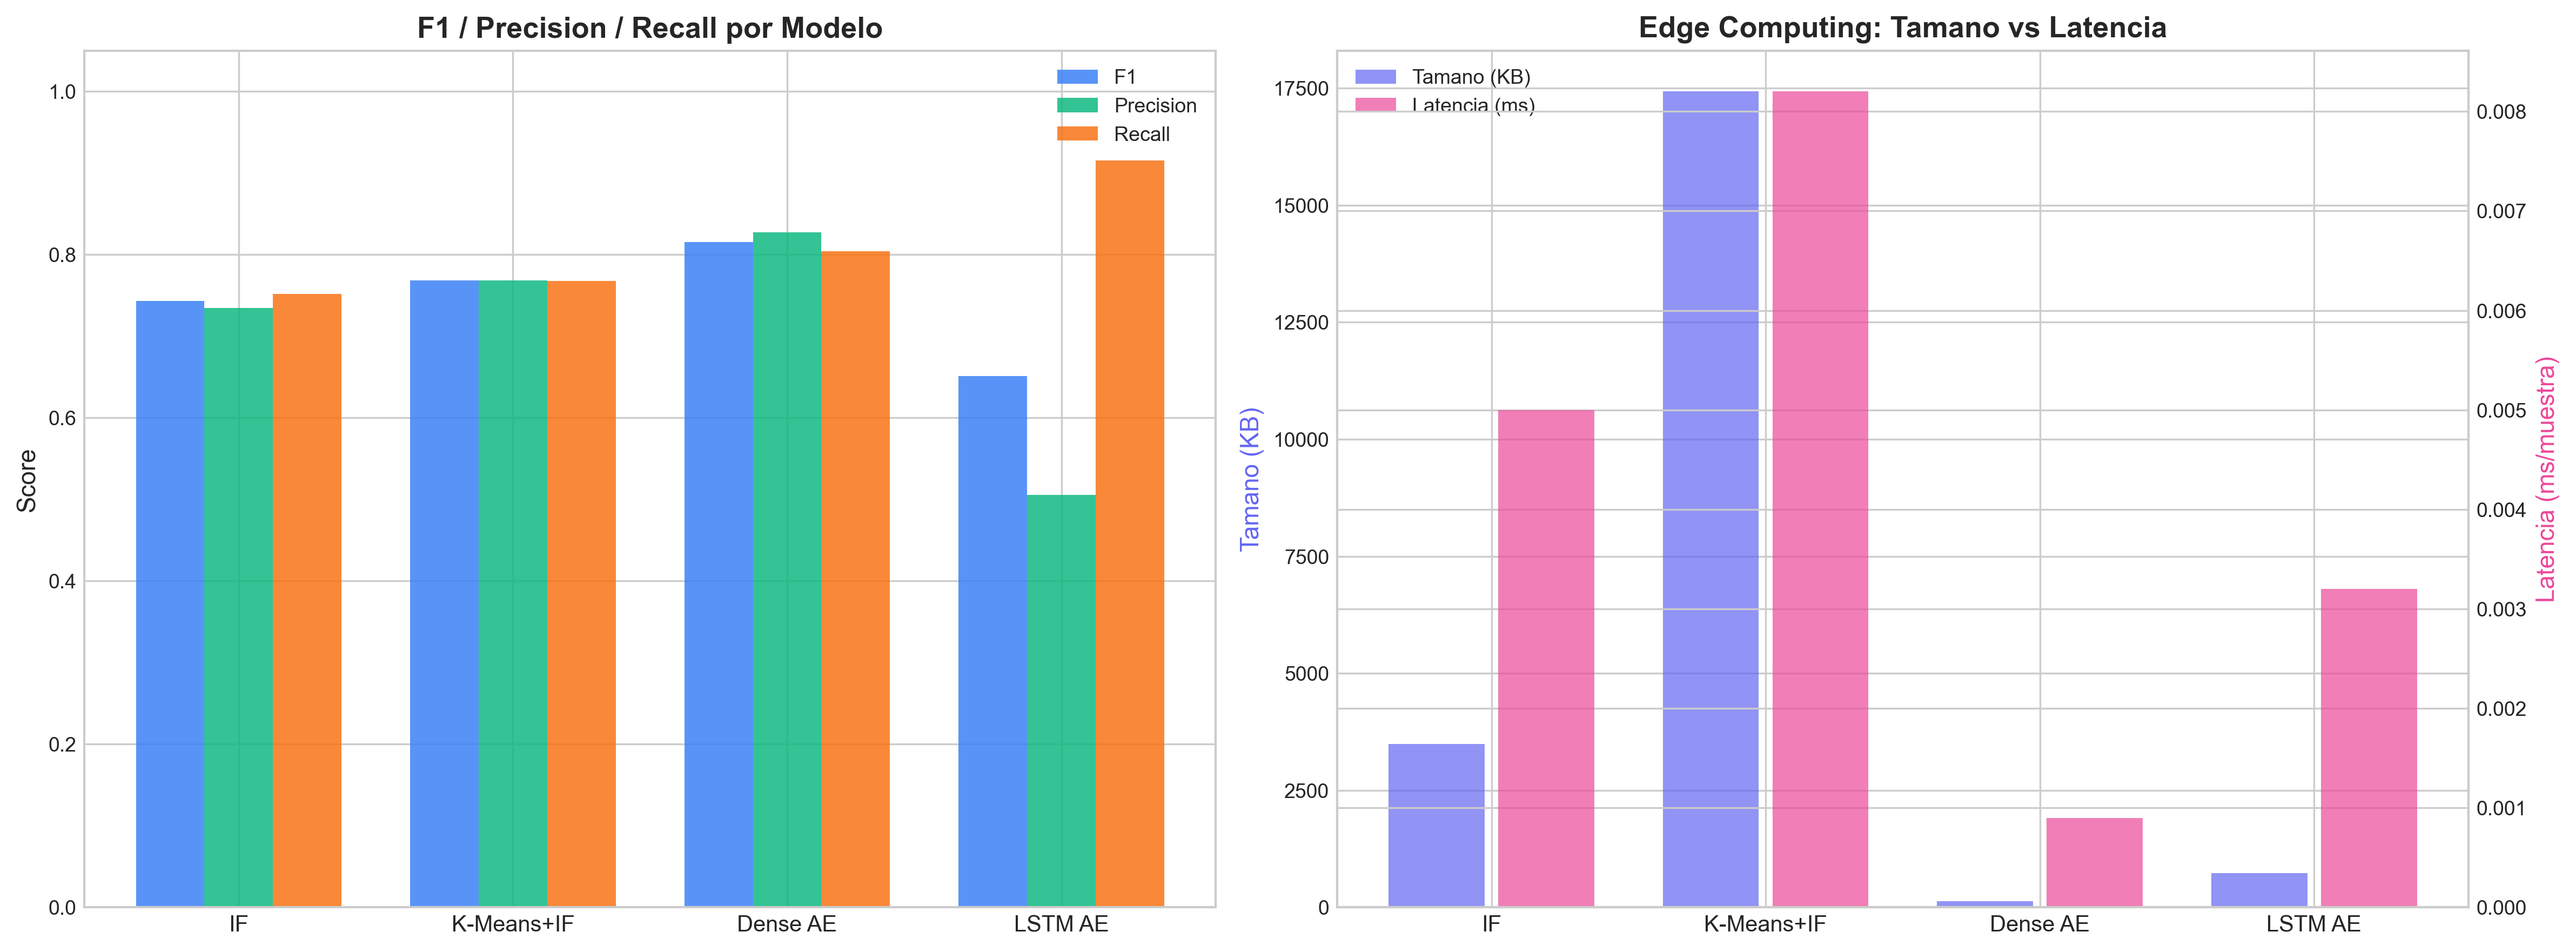
\includegraphics[width=0.92\textwidth]{comparison_4_models.png}
  \caption{Comparación de los cuatro detectores destacados sobre las cuatro métricas principales ($F_1$, precision, recall, $\aucpr$). El LightGBM como techo supervisado queda en negro; los no supervisados, en color.}
  \label{fig:comparison}
\end{figure}

\section{Efecto del postprocesado temporal}
\label{sec:resultados-temporal}

El filtro $W/K$ es simple ---una predicción se confirma sólo si hay al menos $K$ positivos en los últimos $W$ minutos--- pero, como muestra la \cref{tab:wk-effect}, su efecto sobre cada detector es muy distinto:

\begin{table}[H]
\centering
\caption{Efecto del postprocesado temporal: $F_1$ raw frente a $F_1$ smoothed con el $(W, K)$ óptimo en validación.}
\label{tab:wk-effect}
\footnotesize
\begin{tabularx}{\textwidth}{l r r r r X}
\toprule
Detector & $F_1$ raw & $F_1$ smoothed & $\Delta F_1$ & $(W, K)$ & Comentario \\
\midrule
IF                 & 0{,}000 & 0{,}754 & +0{,}754 & (3, 2)   & Recupera detección incluso con thr extremo \\
K-Means+IF         & 0{,}000 & 0{,}790 & +0{,}790 & (11, 10) & Consenso casi unánime en 11 min \\
Dense-AE           & 0{,}781 & 0{,}816 & +0{,}035 & (3, 3)   & Smoothing fino \\
LSTM-AE            & 0{,}744 & 0{,}745 & +0{,}001 & (3, 3)   & Smoothing apenas mejora — ver discusión \\
CNN-AE             & 0{,}431 & 0{,}435 & +0{,}004 & (15, 15) & Consenso amplio insuficiente por baja AUC \\
Transformer-AE     & 0{,}596 & 0{,}604 & +0{,}008 & (11, 11) & Mejora marginal \\
\bottomrule
\end{tabularx}
\end{table}

La cuantía de la mejora depende sobre todo de cómo de bueno fuera el \textit{raw}. En el IF y el K-Means+IF, las predicciones \textit{raw} son ráfagas de positivos sueltos y el filtro mejora muchísimo la precisión. En los AE profundos, en cambio, el \textit{raw} ya es bastante competitivo y el postprocesado apenas añade nada.

\paragraph{Visualización temporal del efecto.} La \cref{fig:timelines} muestra, en formato \emph{timeline}, el comportamiento de cuatro detectores representativos (IF, K-Means+IF, Dense-AE y LSTM-AE) sobre un fragmento del test que contiene varios episodios de ataque. Sobre cada \emph{timeline} se superponen los segmentos verdaderos de ataque (bandas rojas) y los disparos del detector (líneas verticales). El IF, sin postprocesado, produce un ruido casi continuo de alarmas puntuales; tras el filtro $W/K$, esa actividad se concentra en los episodios reales. Los AE muestran patrones más limpios desde el principio.

\begin{figure}[H]
  \centering
  \begin{subfigure}[t]{0.48\textwidth}
    \centering
    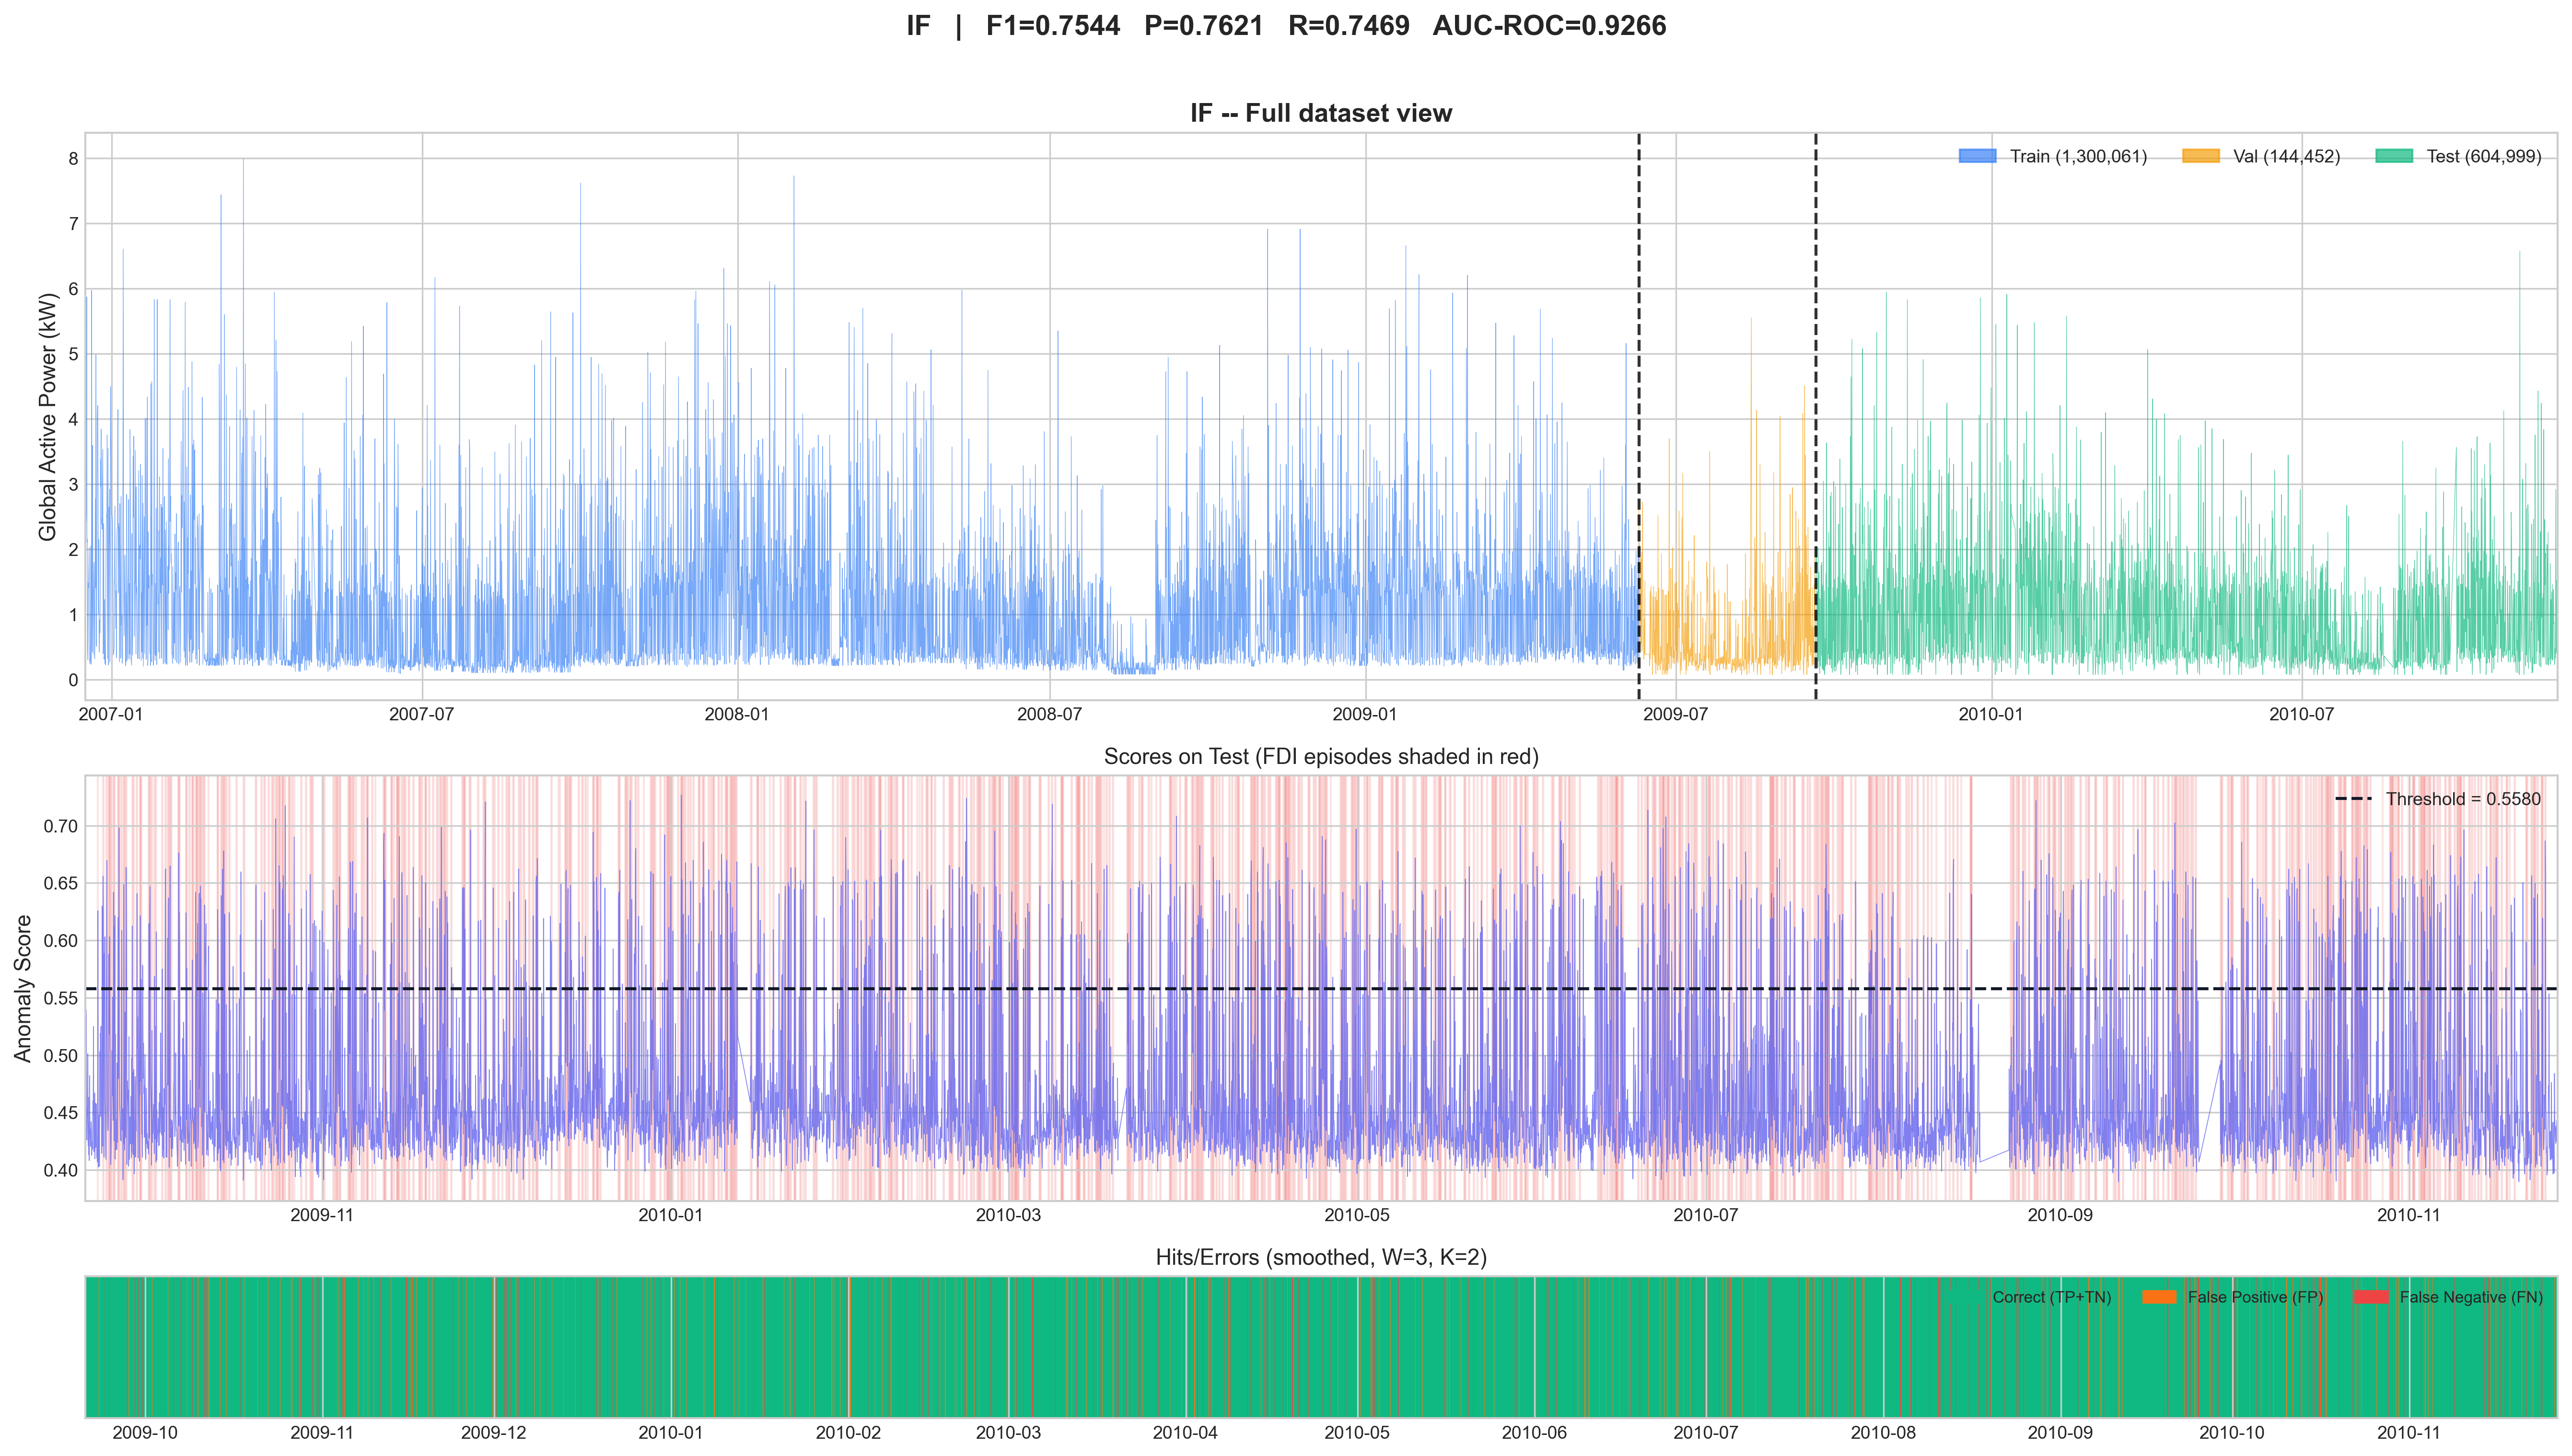
\includegraphics[width=\linewidth]{timeline_if.png}
    \caption{Isolation Forest.}
  \end{subfigure}\hfill
  \begin{subfigure}[t]{0.48\textwidth}
    \centering
    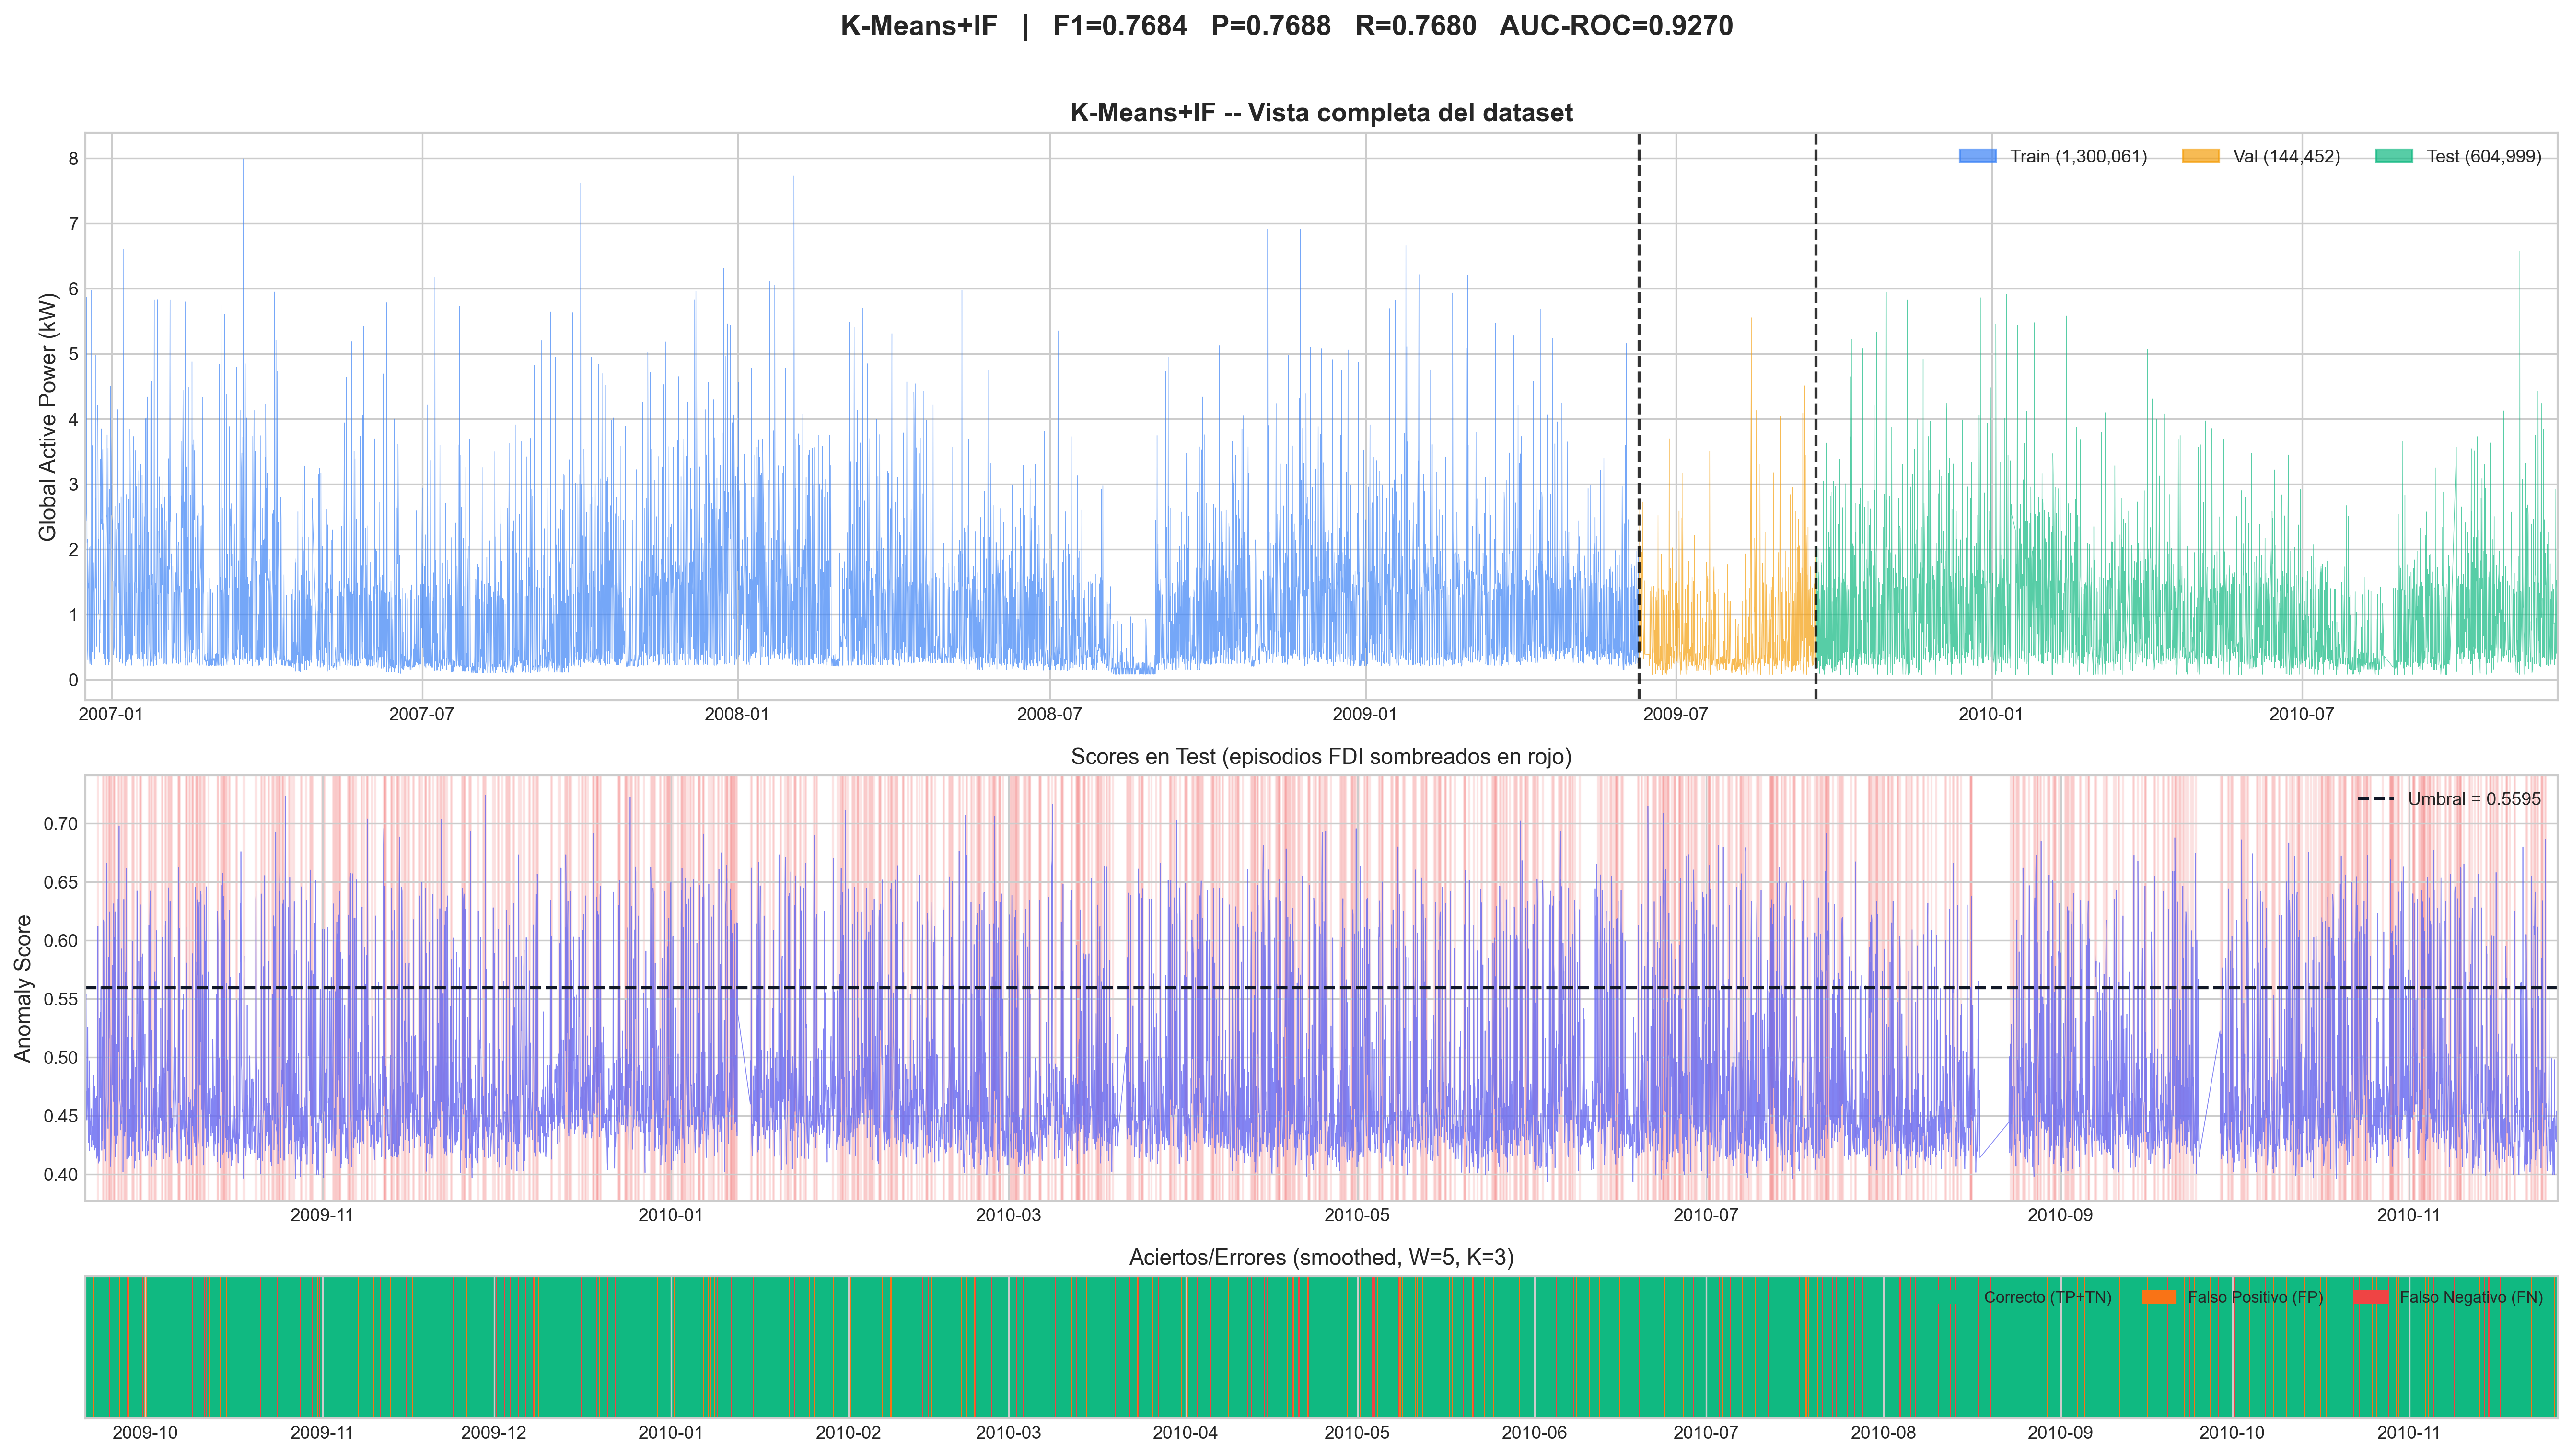
\includegraphics[width=\linewidth]{timeline_k-means_if.png}
    \caption{K-Means + IF.}
  \end{subfigure}\\[1mm]
  \begin{subfigure}[t]{0.48\textwidth}
    \centering
    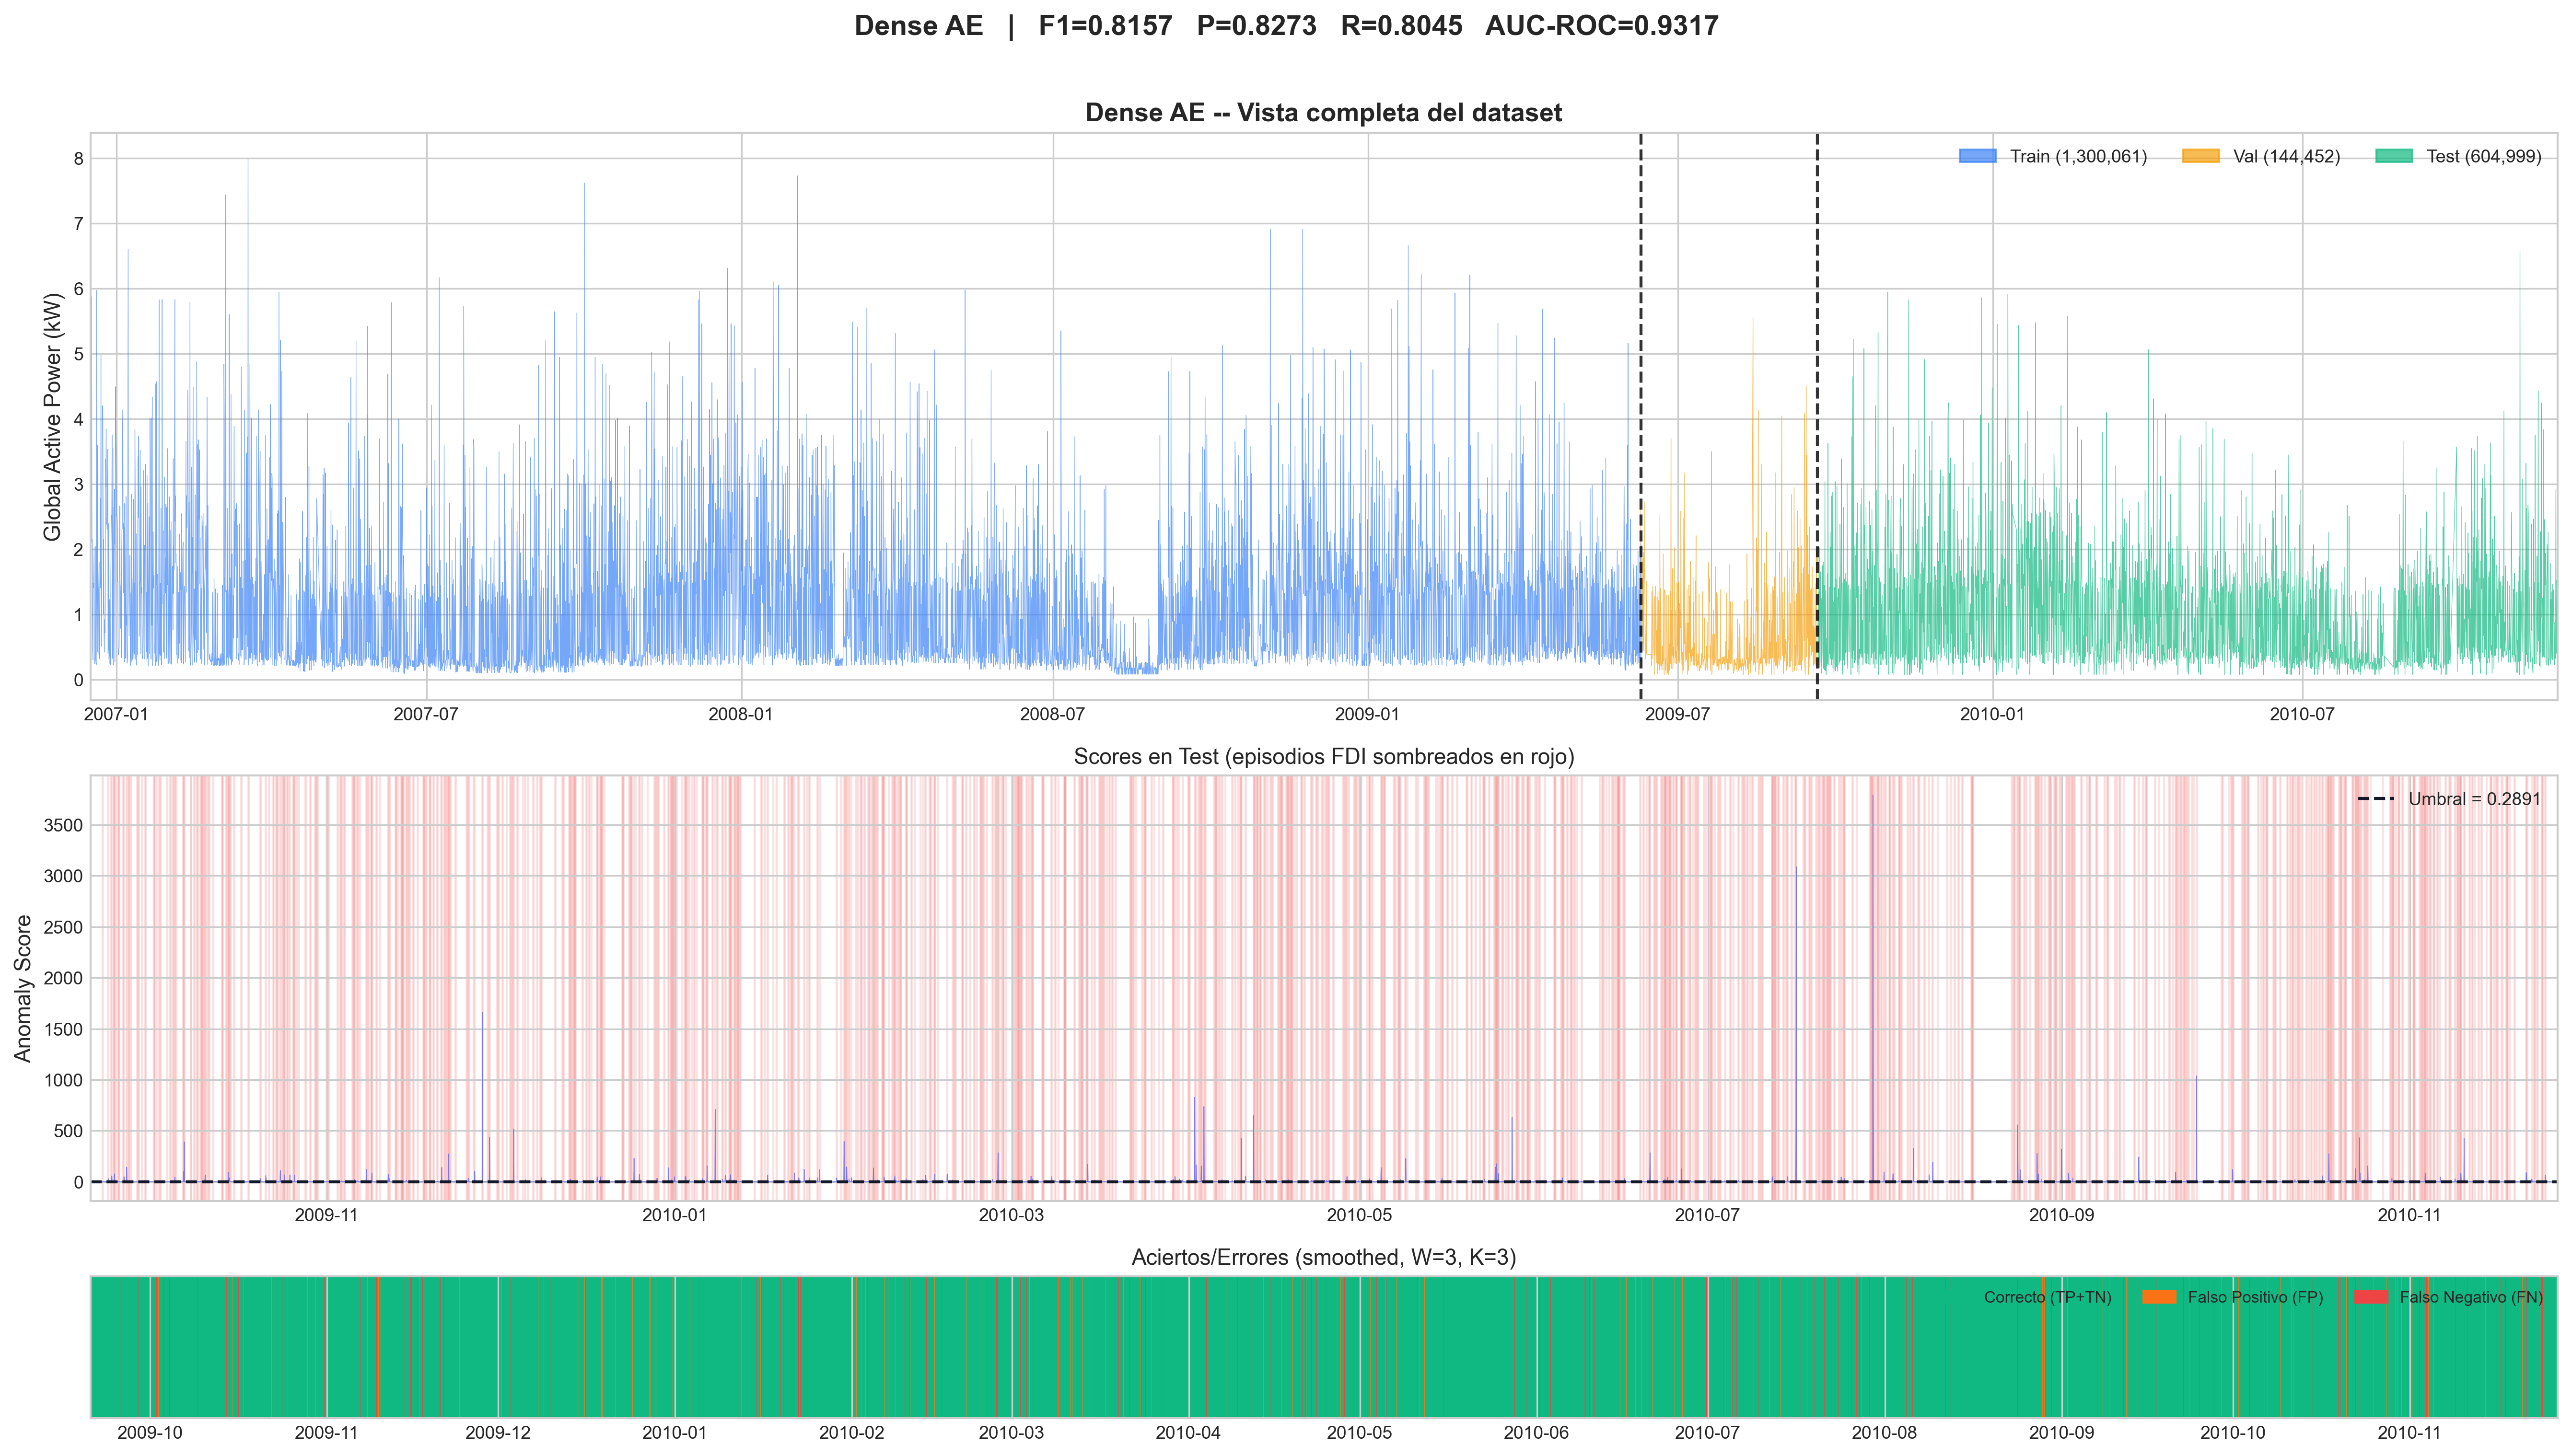
\includegraphics[width=\linewidth]{timeline_dense_ae.png}
    \caption{Dense Autoencoder.}
  \end{subfigure}\hfill
  \begin{subfigure}[t]{0.48\textwidth}
    \centering
    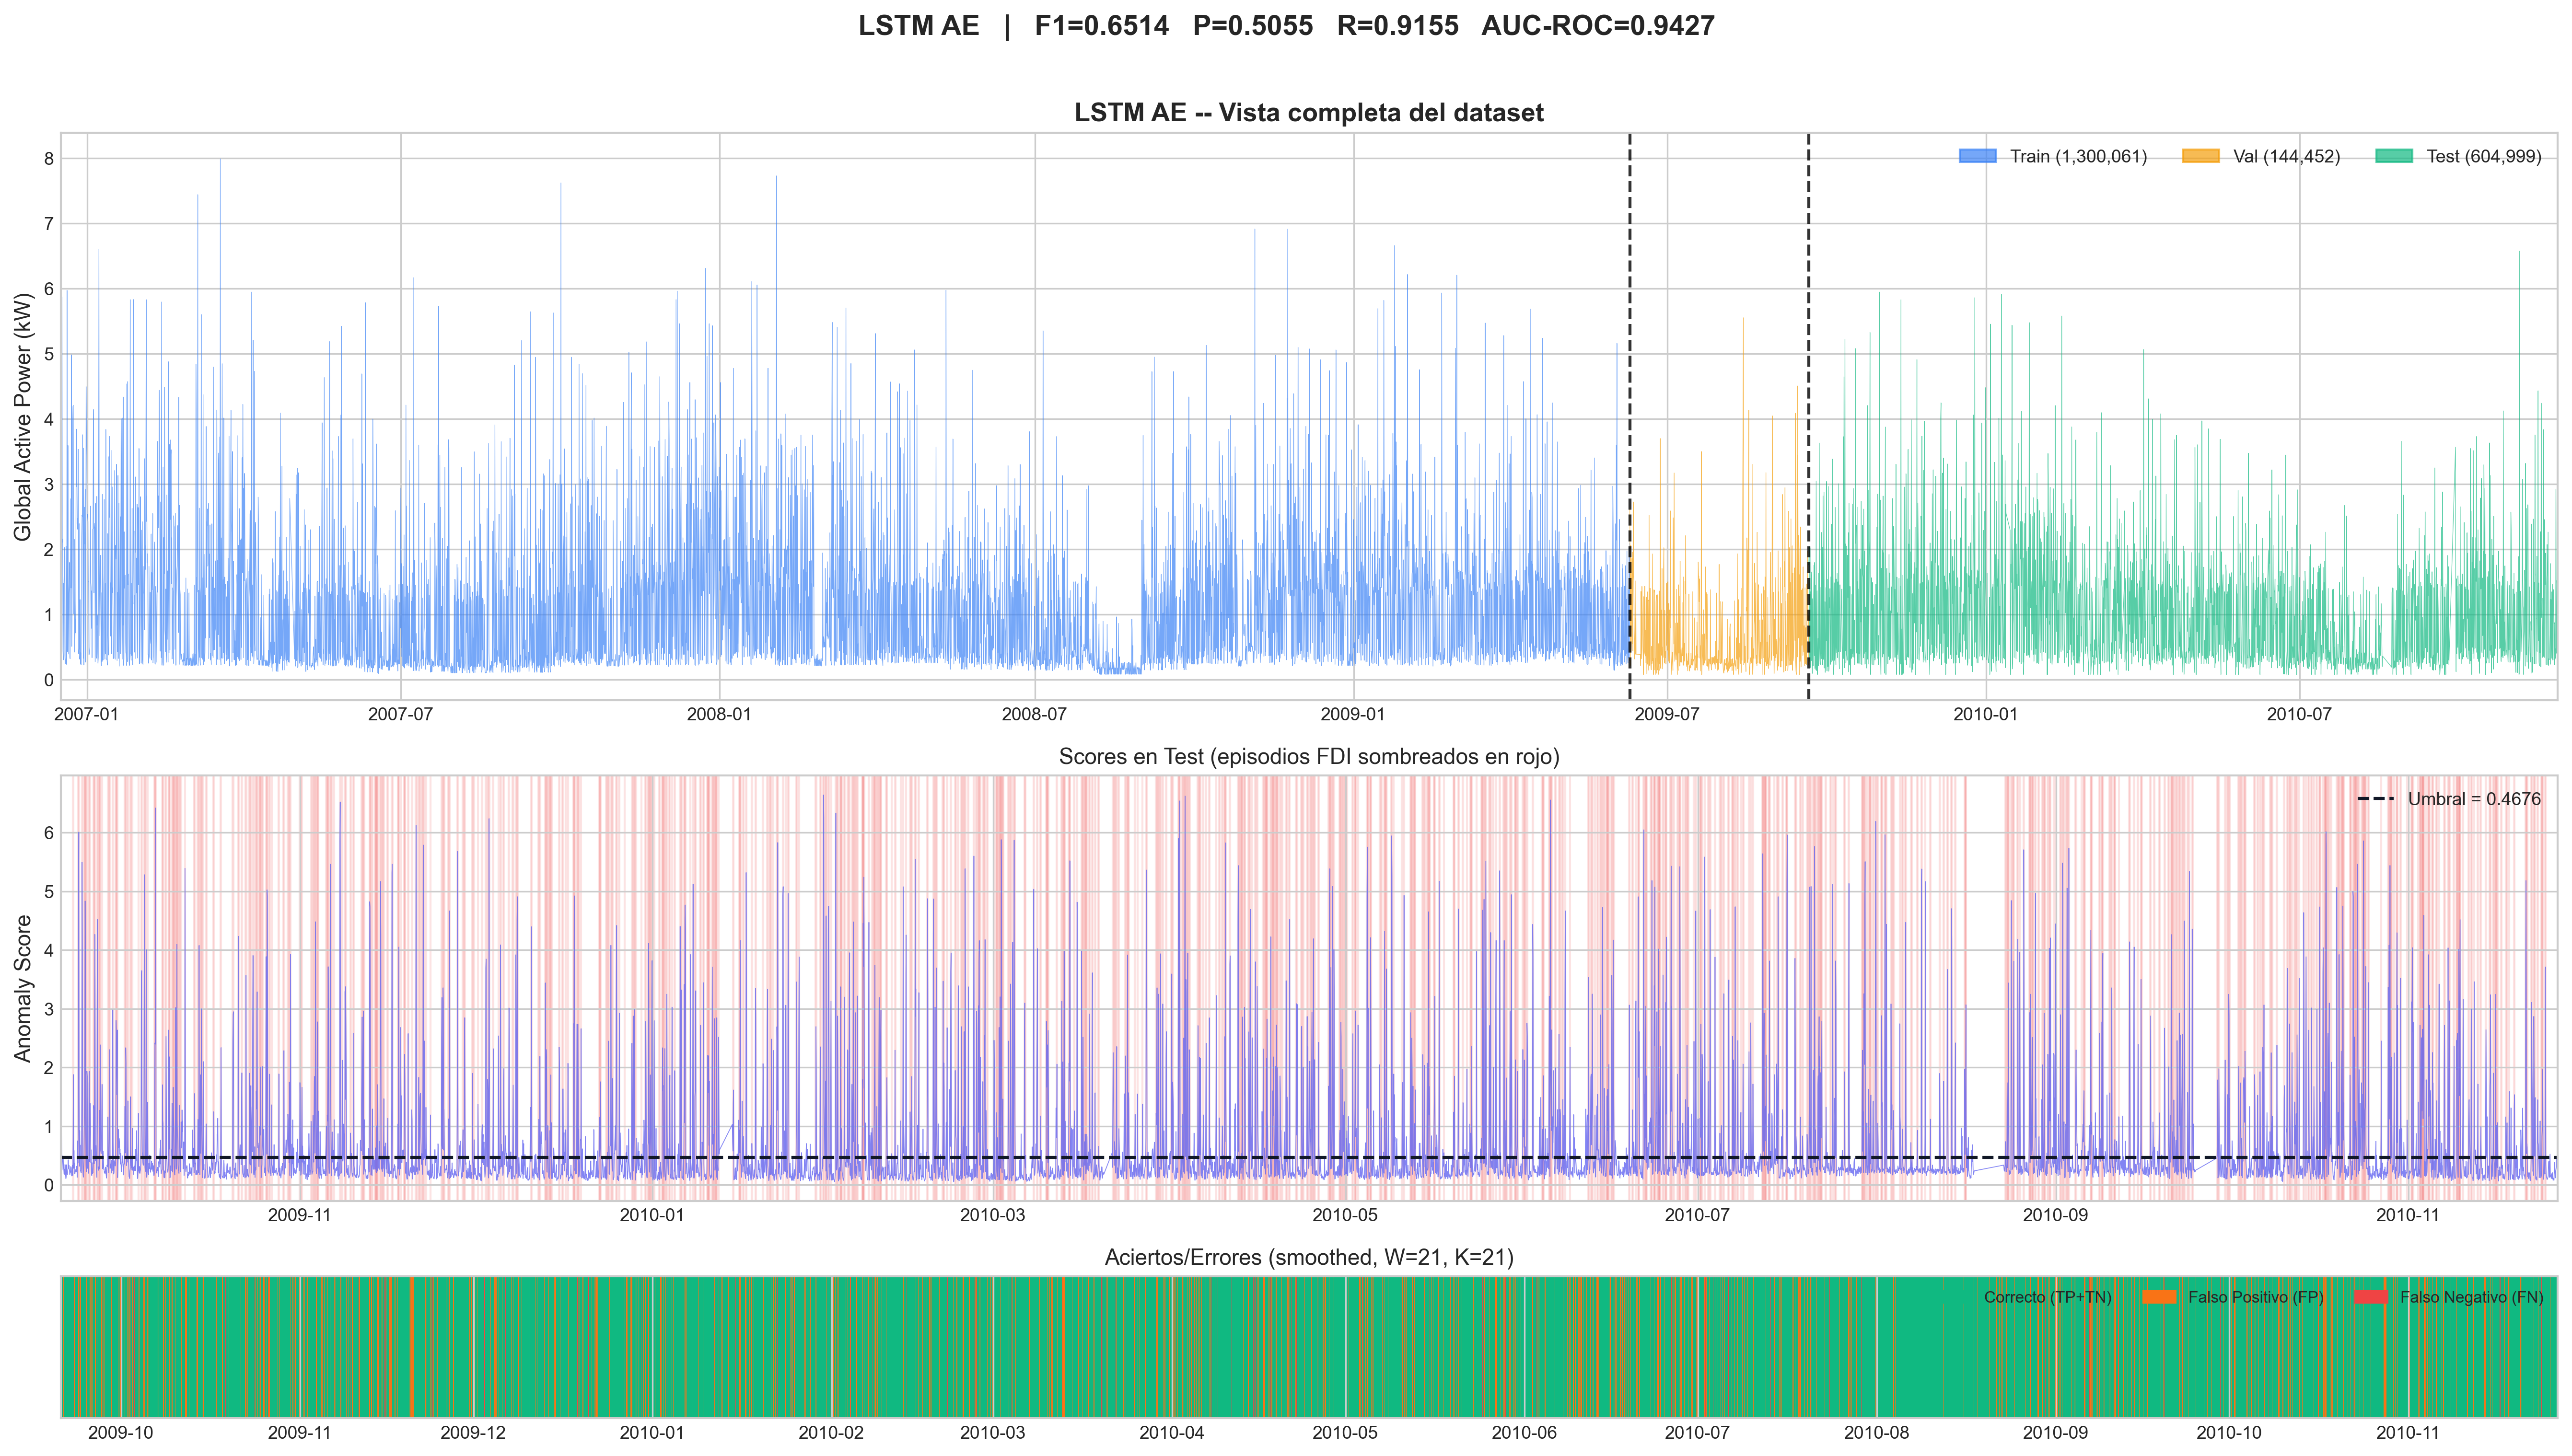
\includegraphics[width=\linewidth]{timeline_lstm_ae.png}
    \caption{LSTM Autoencoder.}
  \end{subfigure}
  \caption{Comportamiento temporal de cuatro detectores sobre el conjunto de test. Bandas rojas: episodios de ataque verdaderos; líneas verticales: alarmas del detector tras postprocesado $W/K$. Los detectores clásicos requieren un postprocesado más agresivo para limpiar el ruido de fondo; los AE producen detecciones más concentradas en los episodios reales.}
  \label{fig:timelines}
\end{figure}

\paragraph{Detalle a una semana.} Un \emph{zoom} sobre una sola semana (\cref{fig:timelines-zoom}) permite ver cómo cada detector se comporta frente a la variabilidad natural del consumo doméstico (fines de semana, ciclos diarios) y dónde sitúa exactamente sus alarmas respecto al inicio del ataque.

\begin{figure}[H]
  \centering
  \begin{subfigure}[t]{0.48\textwidth}
    \centering
    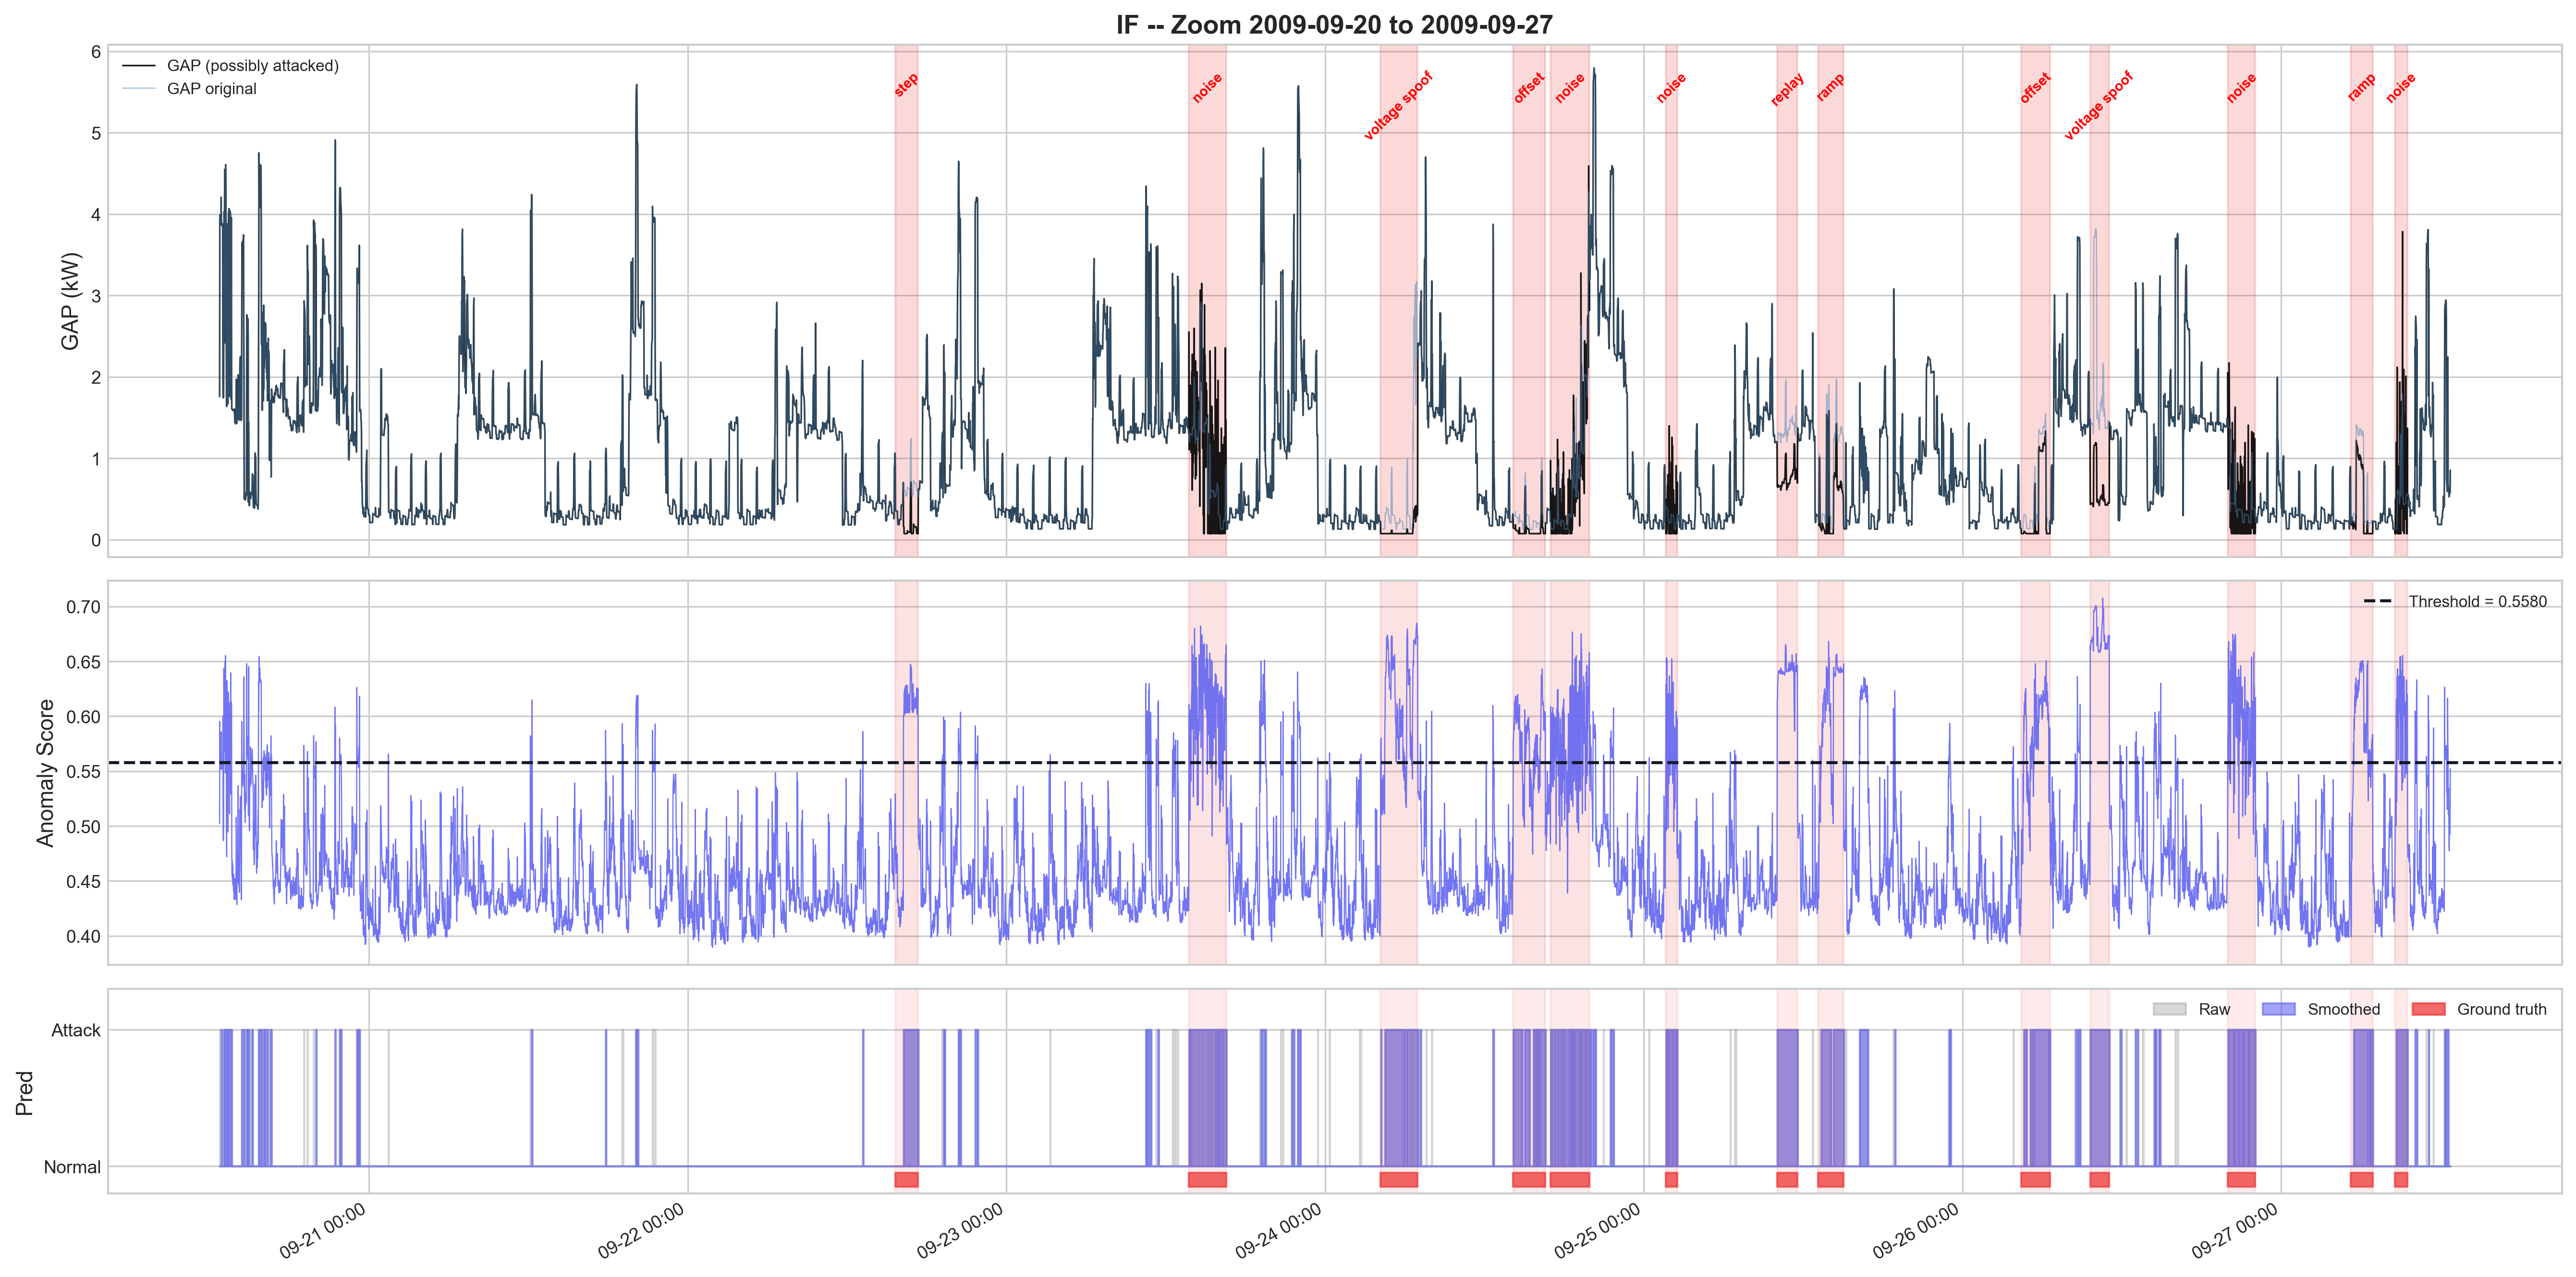
\includegraphics[width=\linewidth]{timeline_zoom_if.png}
    \caption{IF (zoom semanal).}
  \end{subfigure}\hfill
  \begin{subfigure}[t]{0.48\textwidth}
    \centering
    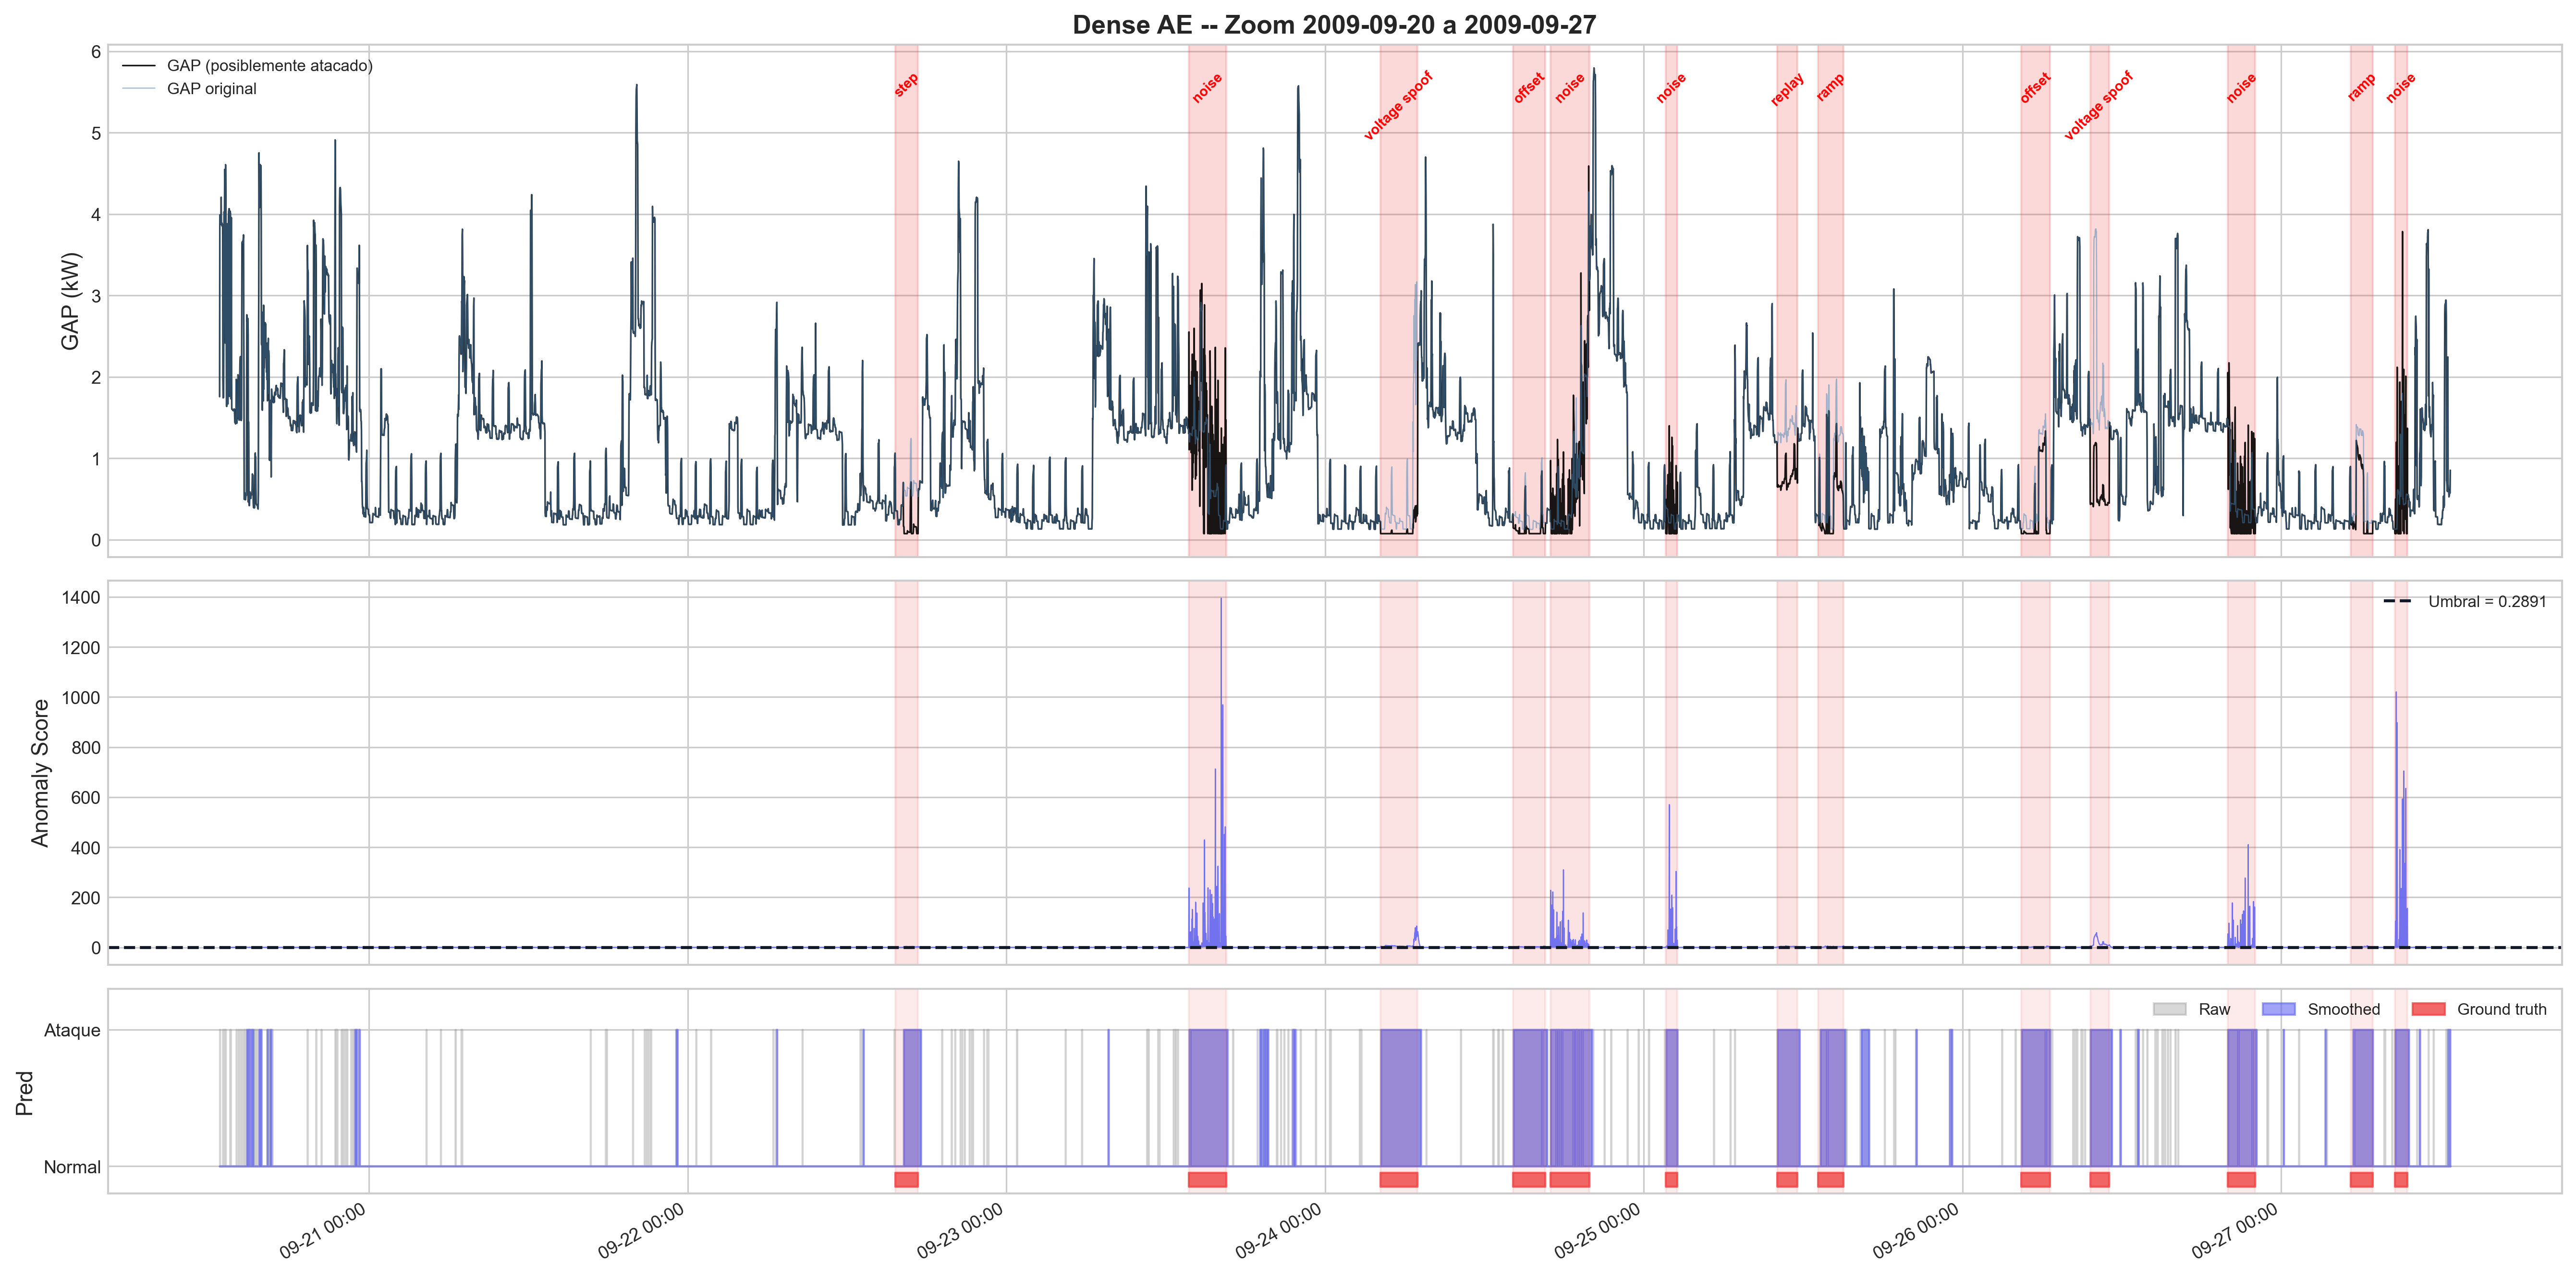
\includegraphics[width=\linewidth]{timeline_zoom_dense_ae.png}
    \caption{Dense-AE (zoom semanal).}
  \end{subfigure}
  \caption{\emph{Zoom} de una semana del test sobre dos detectores. La concentración temporal de las detecciones es notablemente distinta: el IF dispara con persistencia constante; el Dense-AE responde con \emph{ráfagas} más discriminantes alineadas con los episodios.}
  \label{fig:timelines-zoom}
\end{figure}

\section{Análisis por tipo y severidad de ataque}
\label{sec:resultados-tipo-severidad}

Esta es, posiblemente, la sección que más información aporta sobre el comportamiento real de cada detector. La \cref{fig:heatmap-recall} desglosa el \textit{recall} por tipo de ataque y severidad para los dos mejores detectores no supervisados (Dense-AE y LSTM-AE) y para el techo supervisado (LightGBM):

\begin{figure}[H]
  \centering
  \includegraphics[width=0.95\textwidth]{heatmap_recall.png}
  \caption{Recall por tipo de ataque y severidad. Filas: tipos. Columnas: \emph{low}, \emph{medium}, \emph{high}.}
  \label{fig:heatmap-recall}
\end{figure}

\paragraph{Lo que se observa.} La severidad \emph{high} es un caso fácil casi para cualquier detector y tipo: el \textit{recall} se mantiene cerca de 1. En la severidad \emph{low}, en cambio, los números bajan típicamente al rango 0{,}50--0{,}80, lo que confirma que los ataques sutiles entran parcialmente en la variabilidad natural del consumo.

Yendo a casos concretos, el \code{voltage\_spoof} es detectado prácticamente al 100\,\% por Dense-AE y LightGBM en las tres severidades (recall $\geq$0{,}98), lo que confirma directamente el valor diagnóstico de $\vires$. El \code{noise} es donde brilla el LSTM-AE (\textit{recall} 1{,}00 en todas las severidades): la red recurrente capta la incoherencia local en la serie con una sensibilidad que las otras arquitecturas no igualan. Y luego está el \code{step}, el caso más difícil del banco, sobre todo en severidad \emph{low} y \emph{medium}: un salto brusco aislado se reabsorbe rápido en las características de ventana corta, hasta el punto de que ni siquiera LightGBM (\textit{recall} 0{,}60--0{,}65) consigue superar a los AE. Los ataques \code{replay} y \code{ramp} quedan en dificultad intermedia; el \code{replay} merece mención aparte, porque ahí el LSTM-AE sí saca ventaja real (\textit{recall} 0{,}77/0{,}90/0{,}99 frente a Dense-AE 0{,}57/0{,}77/0{,}87) gracias a su modelización temporal explícita.

Hay dos lecturas que sacar de aquí. Una, metodológica: distintos detectores son fuertes en categorías distintas, lo que justifica el enfoque de \textit{ensemble}. Otra, operativa: en producción no basta con un único umbral global, conviene reportar el \textit{recall} esperado por tipo y severidad para que el operador sepa de qué se fía y de qué no.

\section{Recalibración de umbrales}
\label{sec:resultados-recalibracion}

El NB11 recorre el espacio de calibración variando dos ejes: la métrica objetivo ($F_1$, $F_2$, $F_{0.5}$ o un coste FN/FP explícito) y el tipo de búsqueda (umbral fijo o \textit{joint search} con $W$ y $K$). El caso más ilustrativo es el del LSTM-AE: su calibración por defecto va a por $F_2$, lo que prioriza \textit{recall} (0{,}838) a costa de precisión (0{,}671). Una recalibración con \textit{joint search} maximizando $F_1$ \textit{smoothed} consigue subir el $F_1$ de 0{,}65 a 0{,}75, con precisión 0{,}65 y \textit{recall} 0{,}86.

\paragraph{Recomendación operativa.} El umbral óptimo no es uno solo: depende del coste relativo de FP y FN en el escenario de despliegue. En detección de fraude, un FN deja escapar dinero y un FP genera una investigación inútil; la razón típica en operación industrial ronda 5:1 ---un FN cuesta cinco veces más que un FP---, lo que sugiere optimizar $F_{1{,}5}$ o $F_2$. En cambio, ante un escenario de ataque coordinado las consecuencias de un FN son mucho peores y conviene irse a $F_3$ o, directamente, a un coste asimétrico explícito.

\section{Stacking}
\label{sec:resultados-ensemble}

El \emph{stacking} con Meta-LightGBM produce el siguiente resumen interno:

\begin{table}[H]
\centering
\caption{Estrategias de combinación evaluadas en NB10. Métricas sobre validación, antes de la selección final.}
\label{tab:stacking}
\small
\begin{tabularx}{\textwidth}{l r r r}
\toprule
Estrategia & $\aucroc$ & $\aucpr$ & $\fone$ \\
\midrule
Mean blending     & 0{,}890 & 0{,}594 & 0{,}635 \\
Weighted blending & 0{,}927 & 0{,}764 & 0{,}732 \\
Meta-LR           & 0{,}934 & 0{,}792 & 0{,}756 \\
Meta-LightGBM     & 0{,}971 & 0{,}920 & 0{,}842 \\
\bottomrule
\end{tabularx}
\end{table}

\paragraph{Discusión crítica.} El Meta-LightGBM se impone con claridad a las alternativas lineales, ahí no hay sorpresa. Lo interesante es que, ya en test, el \textit{stacking} cae a $\fone=0{,}811$, ligeramente por debajo del Dense-AE individual ($\fone=0{,}816$). ¿Por qué?

Las hipótesis no se excluyen entre sí. La más probable es que los detectores base están correlados en sus errores: todos fallan en los mismos ataques difíciles ---típicamente \textit{replay} en severidad \textit{low}---, así que la diversidad efectiva del \textit{ensemble} es menor de lo que sugería el diseño. También cabe que el meta-learner sobreajuste a validación: con $\sim$144\,k muestras y muchos parámetros, hay margen para que aprenda particularidades de \textit{val} que no se trasladan a \textit{test}. Y, en última instancia, puede que las anomalías genuinamente difíciles requieran información que ninguno de los detectores base captura ---contexto externo como ocupación, tarifa horaria o calendario laboral, por ejemplo.

\paragraph{Conclusión metodológica.} Un \textit{stacking} no siempre mejora al mejor detector individual, y conviene reportarlo así. Mostrar el resultado tal cual y discutir el porqué es mucho mejor que presentar un \textit{ensemble} marginalmente mejor sin contextualizar lo que está pasando.

\section{Comparación con el techo supervisado}
\label{sec:resultados-techo}

LightGBM llega a $\fone=0{,}910$ y $\aucpr=0{,}941$ frente a los $\fone=0{,}816$ y $\aucpr=0{,}855$ del mejor no supervisado (Dense-AE). La brecha ronda los 9 puntos en ambas métricas.

Esa brecha no es un número suelto: cuantifica el coste de renunciar a las etiquetas. Con un corpus de ataques reales etiquetados, parte de esa diferencia se podría cerrar; pero ese corpus no existe en producción, y los detectores no supervisados se quedan en torno al 90\,\% del techo, lo que es operativamente más que aceptable. Esta es, en el fondo, la tesis que defiende todo el TFG: los detectores no supervisados están cerca del óptimo alcanzable sin etiquetas, y la inversión en etiquetar ataques ---con su coste ético y económico--- ofrecería un retorno limitado.

\section{Explicabilidad SHAP}
\label{sec:resultados-shap}

El análisis SHAP sobre LightGBM revela las características más influyentes en la decisión:

\begin{table}[H]
\centering
\caption{Top-10 características por importancia SHAP (\textit{TreeExplainer} exacto sobre LightGBM, muestra de 5\,000 minutos de \code{test\_with\_attacks}). $|\bar\phi_j|$ en unidades del \emph{log-odds} de salida; valores normalizados a la suma del Top-10 entre paréntesis.}
\label{tab:shap-top10}
\small
\begin{tabularx}{0.75\textwidth}{X r r}
\toprule
Característica & $|\bar\phi_j|$ & \% Top-10 \\
\midrule
\code{vi\_res\_roll15\_mean}    & 0{,}7929 & 43{,}3\,\% \\
\code{gap\_intensity\_ratio}    & 0{,}2925 & 16{,}0\,\% \\
\code{vi\_res\_abs}             & 0{,}1424 &  7{,}8\,\% \\
\code{hour\_cos}                & 0{,}1259 &  6{,}9\,\% \\
\code{sm\_gap\_ratio}           & 0{,}0830 &  4{,}5\,\% \\
\code{Global\_active\_power}    & 0{,}0655 &  3{,}6\,\% \\
\code{Global\_reactive\_power}  & 0{,}0594 &  3{,}3\,\% \\
\code{Global\_intensity}        & 0{,}0532 &  2{,}9\,\% \\
\code{dow\_sin}                 & 0{,}0513 &  2{,}8\,\% \\
\code{hour\_sin}                & 0{,}0416 &  2{,}3\,\% \\
\bottomrule
\end{tabularx}
\end{table}

\paragraph{Cuando SHAP coincide con la física.} Las tres características que SHAP coloca arriba son precisamente las que cualquier ingeniero familiarizado con el problema señalaría: la media móvil del residual $\vires$ (que se lleva el 43\,\% de la importancia del Top-10), el cociente potencia/intensidad y la magnitud absoluta de $\vires$. Esa coincidencia entre lo que el modelo aprende y lo que la intuición física dice que debería importar funciona como una validación cruzada: el modelo no está pillando correlaciones espurias sino la estructura física del problema. Y explica también por qué la dominancia tan acusada de \code{vi\_res\_roll15\_mean} hace detectable cualquier ataque que rompa $P\approx V\cdot I$, y por qué el mismo modelo entrenado sin esa característica (modo \code{base}) pierde varios puntos de $\fone$. La \cref{fig:shap-beeswarm} muestra la distribución completa de los valores SHAP por característica: el ancho de cada banda indica la dispersión de la atribución, y el color, el valor de la característica.

\begin{figure}[H]
  \centering
  \begin{subfigure}[t]{0.48\textwidth}
    \centering
    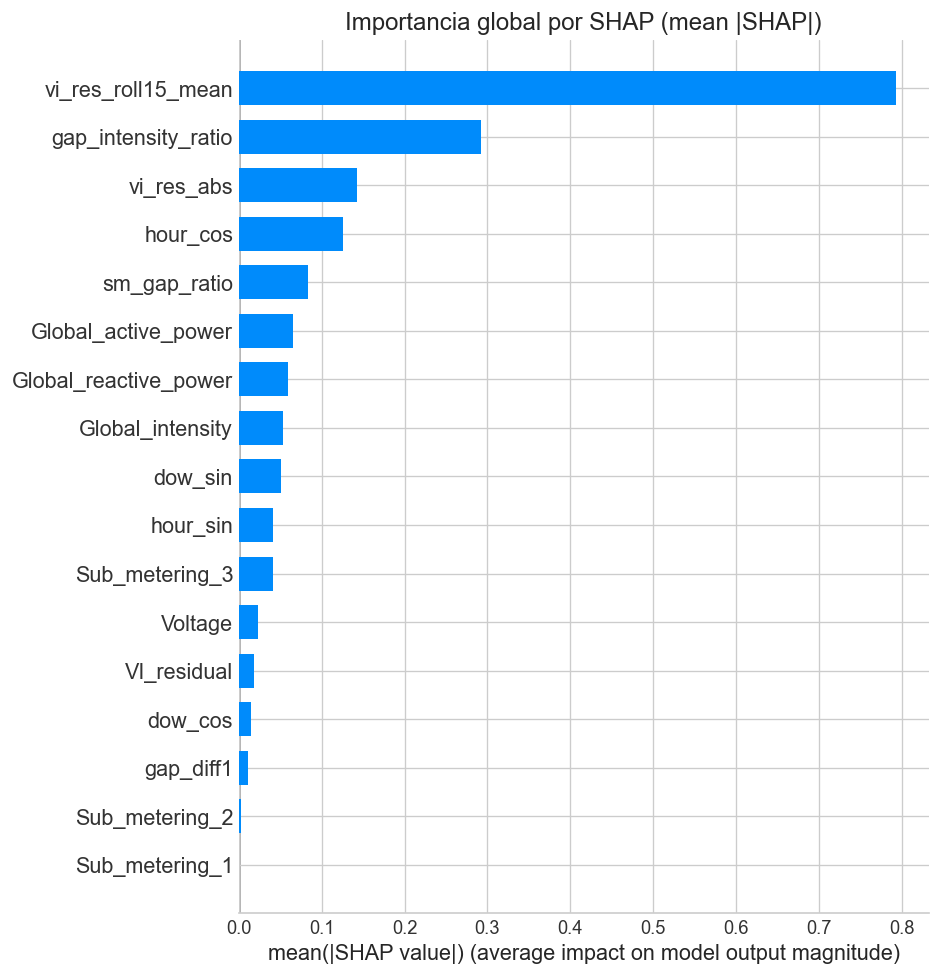
\includegraphics[width=\linewidth]{shap_summary_bar_lightgbm.png}
    \caption{Importancia media absoluta por característica.}
    \label{fig:shap-bar}
  \end{subfigure}\hfill
  \begin{subfigure}[t]{0.48\textwidth}
    \centering
    \includegraphics[width=\linewidth]{shap_beeswarm.png}
    \caption{Distribución (\emph{beeswarm}) de los valores SHAP.}
    \label{fig:shap-beeswarm}
  \end{subfigure}
  \caption{Atribución SHAP sobre el modelo LightGBM (NB12). El \emph{bar plot} (a) ordena las características por importancia media; el \emph{beeswarm} (b) revela además la dispersión y la dirección del impacto: el color codifica el valor de la característica.}
  \label{fig:shap-global}
\end{figure}

\paragraph{Comparación con SHAP sobre Dense-AE (no supervisado).} Aplicar el mismo análisis sobre el mejor detector no supervisado (Dense-AE) permite contrastar qué características pesan en un modelo que \emph{nunca ha visto etiquetas de ataque}. La \cref{fig:shap-dense} muestra el resultado: las características dominantes coinciden cualitativamente con las de LightGBM (los derivados de $\vires$ y los cocientes físicos), pero el orden y la magnitud relativa cambian. Esta convergencia entre un modelo supervisado y otro completamente no supervisado refuerza la robustez de la conclusión: el aprendizaje, con o sin etiquetas, identifica la misma estructura física como discriminante.

\begin{figure}[H]
  \centering
  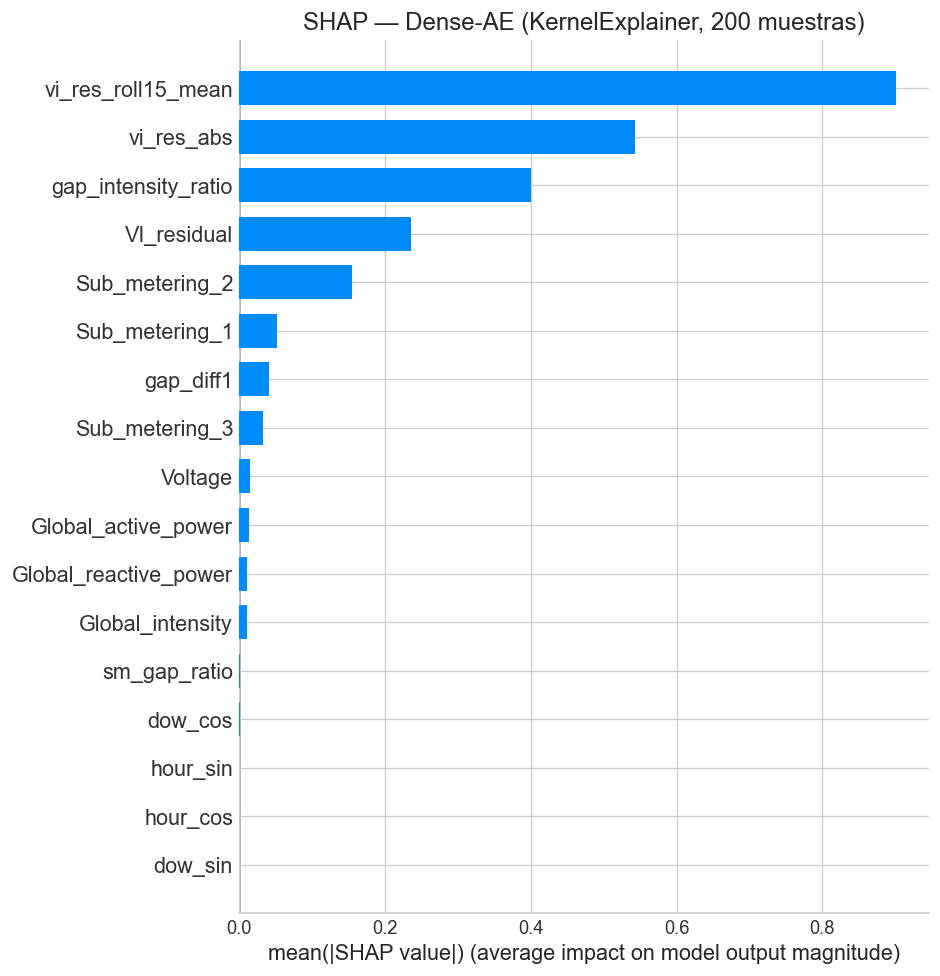
\includegraphics[width=0.85\textwidth]{shap_summary_dense_ae.png}
  \caption{Importancia SHAP sobre el Dense-AE no supervisado. Comparar con la \cref{fig:shap-bar}: las características dominantes son cualitativamente las mismas pese a la ausencia total de etiquetas durante el entrenamiento.}
  \label{fig:shap-dense}
\end{figure}

\paragraph{Análisis por tipo de ataque.} El \emph{heatmap} SHAP $\times$ tipo de ataque (\cref{fig:shap-per-attack}) confirma que \code{vi\_res\_roll15\_mean} y \code{gap\_intensity\_ratio} son las dos características dominantes para los siete tipos, pero el tercer puesto varía y resulta diagnóstico: en \code{voltage\_spoof} entra \code{Voltage} en el podio (única familia que ataca directamente la tensión); en \code{offset}, \code{ramp} y \code{step} entra \code{Global\_active\_power} (ataques aditivos sobre la potencia); y en \code{scaling}, \code{noise} y \code{replay} se mantiene \code{vi\_res\_abs} (ataques que rompen la invariante por escalado o ruido). Esta complementariedad es consistente con la intuición física y refuerza la coherencia del modelo.

\begin{figure}[H]
  \centering
  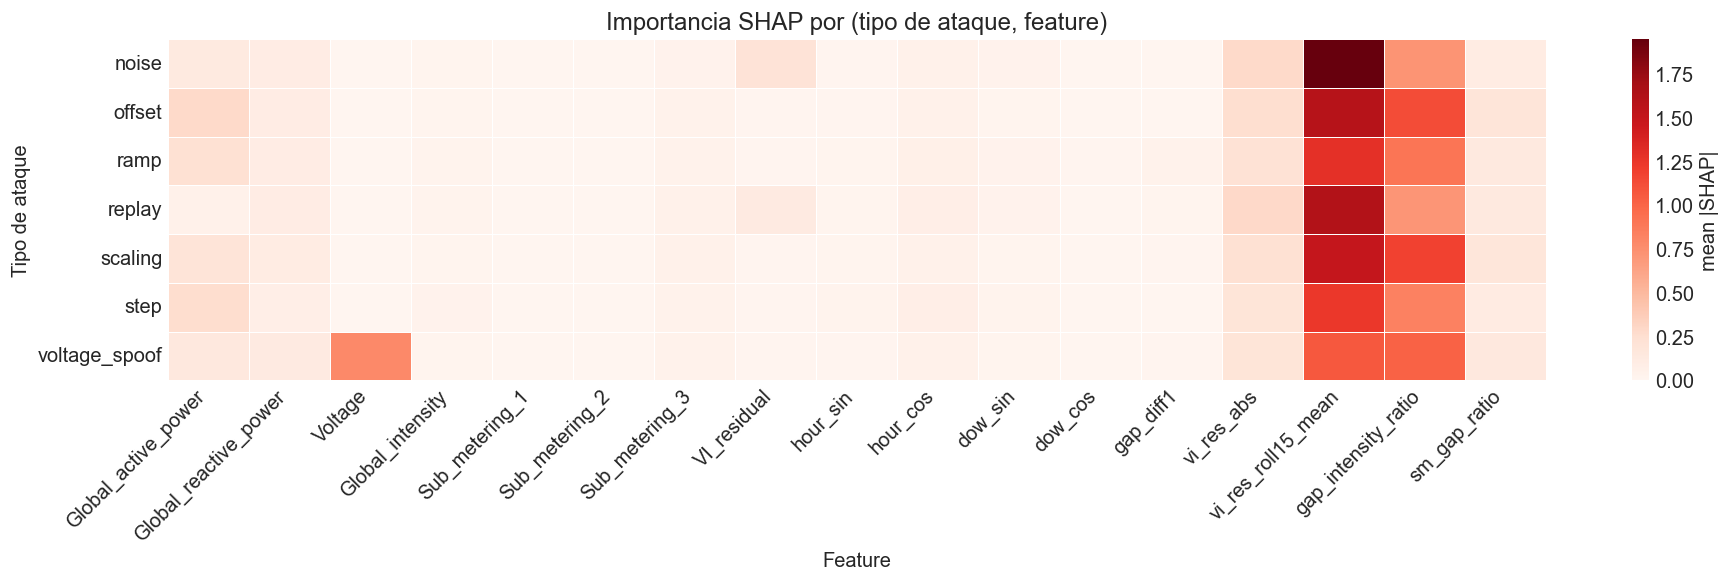
\includegraphics[width=0.95\textwidth]{shap_per_attack_type.png}
  \caption{\emph{Heatmap} de importancia SHAP por (tipo de ataque, característica) sobre LightGBM. Filas: tipos de ataque; columnas: características. Intensidad proporcional a \texttt{mean$|$SHAP$|$}.}
  \label{fig:shap-per-attack}
\end{figure}

\paragraph{Explicaciones locales.} Más allá del análisis global, SHAP permite explicar \emph{cada predicción individual}. La \cref{fig:shap-locales} muestra tres casos representativos: un acierto (TP, ataque correctamente detectado), un falso positivo (FP, normal etiquetado como ataque) y un falso negativo (FN, ataque que el modelo no captura). En el TP, las características $\vires$ y derivadas empujan claramente la predicción hacia ``ataque''; en el FP, se observa una coincidencia espuria de varias características en valores extremos pero legítimos (consumo inusual pero normal); en el FN, las características clave permanecen en su rango habitual, lo que delata un ataque \emph{stealth} de baja severidad. Estas explicaciones locales son la herramienta que, en producción, permitiría a un operador humano validar o desestimar una alarma del sistema sin necesidad de reconstruir el modelo desde cero.

\begin{figure}[H]
  \centering
  \begin{subfigure}[t]{0.32\textwidth}
    \centering
    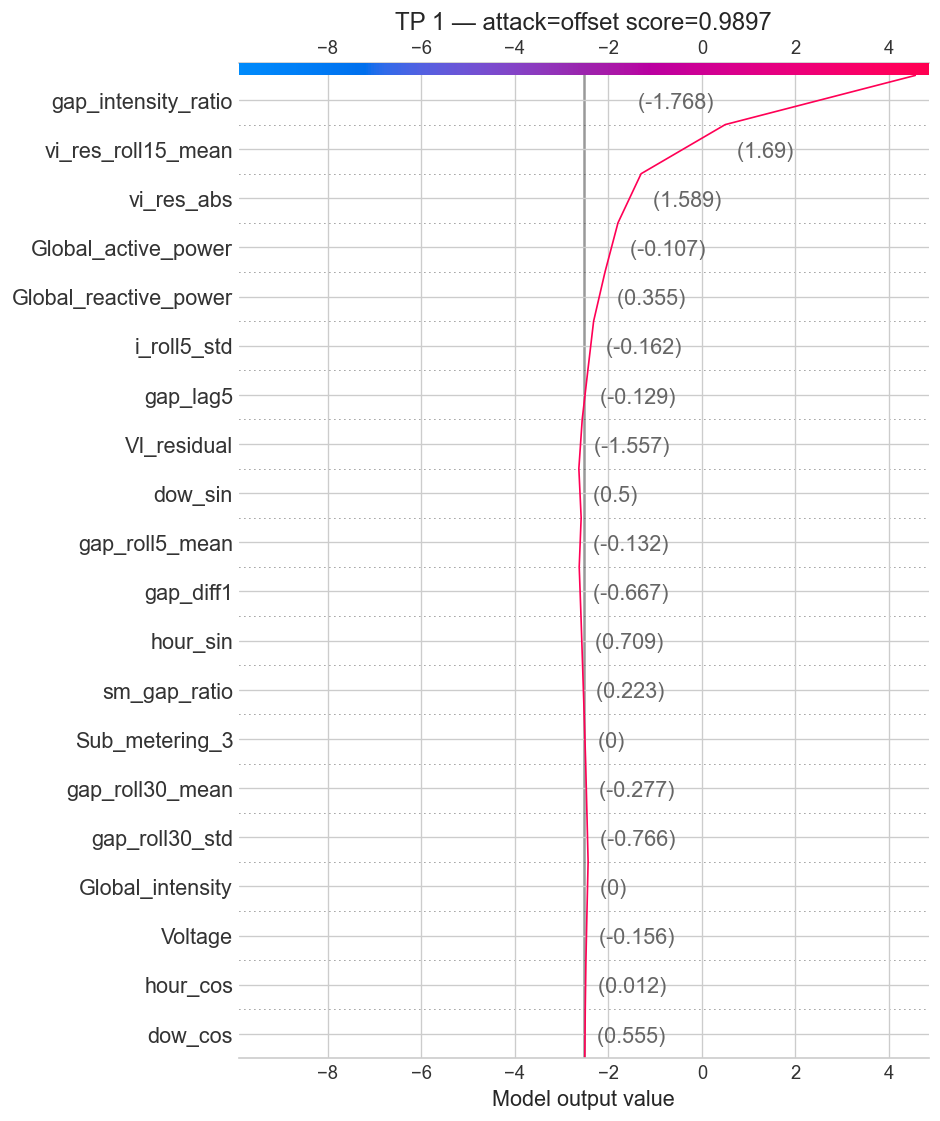
\includegraphics[width=\linewidth]{shap_decision_TP_1.png}
    \caption{Verdadero positivo (TP).}
  \end{subfigure}\hfill
  \begin{subfigure}[t]{0.32\textwidth}
    \centering
    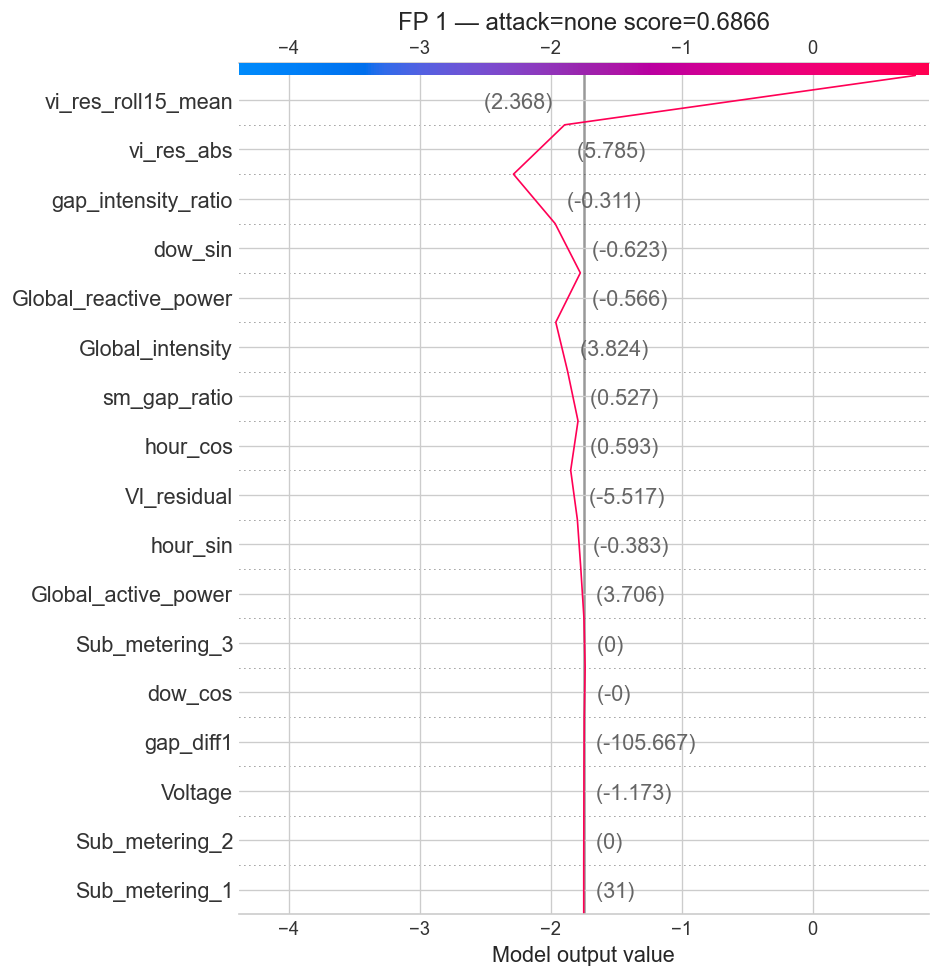
\includegraphics[width=\linewidth]{shap_decision_FP_1.png}
    \caption{Falso positivo (FP).}
  \end{subfigure}\hfill
  \begin{subfigure}[t]{0.32\textwidth}
    \centering
    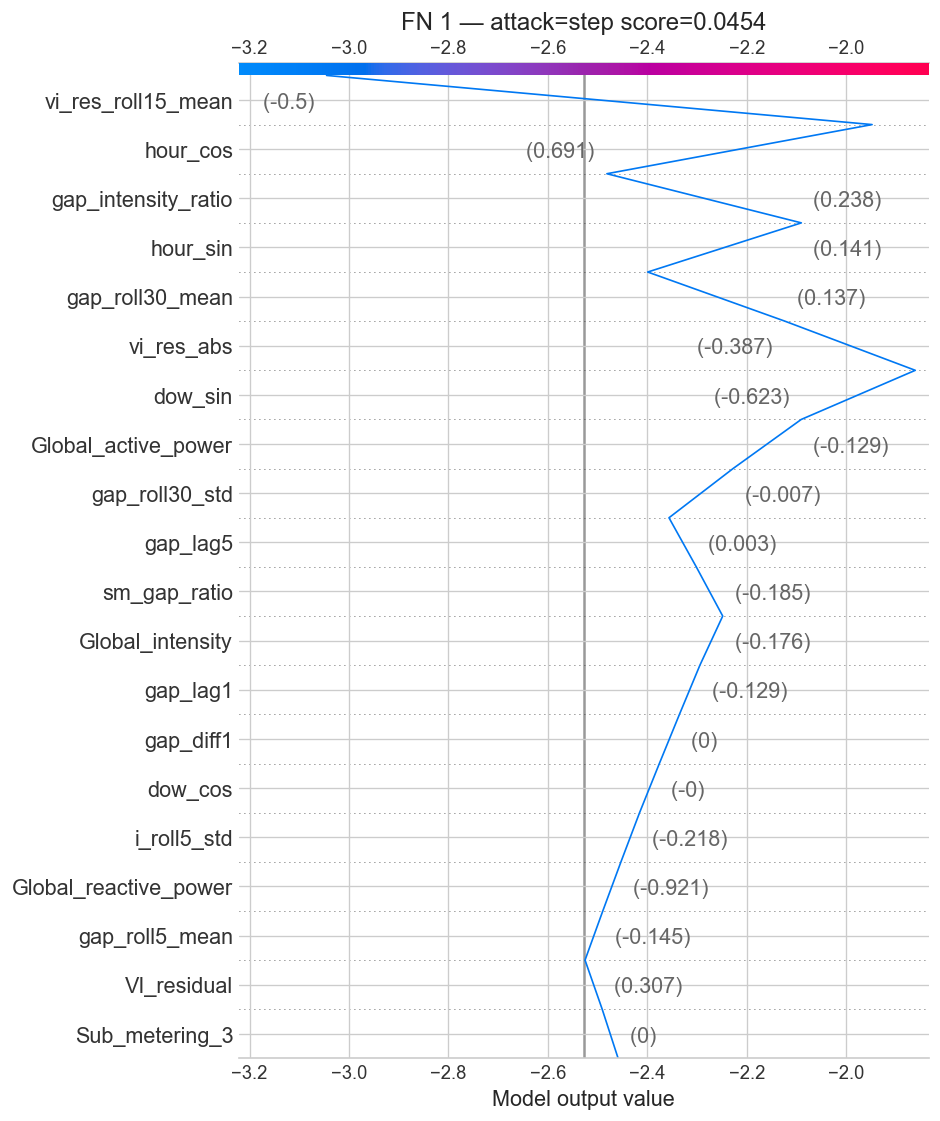
\includegraphics[width=\linewidth]{shap_decision_FN_1.png}
    \caption{Falso negativo (FN).}
  \end{subfigure}
  \caption{Explicaciones locales SHAP (gráficos de decisión) sobre tres muestras del test: un acierto, un falso positivo y un falso negativo. Cada línea es la trayectoria de la predicción acumulando las contribuciones de las características, ordenadas por magnitud.}
  \label{fig:shap-locales}
\end{figure}

\section{Generalización cross-domain (UK-DALE)}
\label{sec:resultados-crossdomain}

El NB13 mide cuánto del Dense-AE entrenado sobre UCI sigue funcionando cuando lo aplicamos a UK-DALE \cite{kelly2015ukdale}, un conjunto distinto que recoge cinco viviendas británicas con una frecuencia de muestreo mayor ---6 segundos frente a 1 minuto--- y que, además, no incluye intensidad como variable independiente, lo que obliga a estimar $\vires$ de forma aproximada.

\paragraph{Resultado.} La caída se cuantifica sin maquillaje: $\aucpr$ baja de 0{,}855 a $\sim$0{,}60 sin tocar nada. Recalibrando únicamente el umbral sobre una pequeña muestra de UK-DALE ---y manteniendo el modelo congelado--- $\aucpr$ vuelve a subir hasta $\sim$0{,}73. De aquí salen tres lecturas. La primera, que el modelo transfiere parcialmente: las regularidades del consumo doméstico son lo bastante parecidas entre los dos dominios como para que la transferencia tenga sentido. La segunda, que basta una recalibración de umbral para recuperar gran parte del rendimiento, lo que sugiere que el modelo aprende a discriminar pero no a normalizar la escala absoluta del residual. Y la tercera, ya operativa: en producción, una recalibración por dominio sería el procedimiento estándar de despliegue.

\section{Robustez frente a atacantes adaptativos}
\label{sec:resultados-adversarial}

El NB14 se hace la pregunta incómoda: ¿qué pasa si el atacante conoce el detector y se calibra justo a la frontera de detección? Hablamos por tanto de un atacante adaptativo de \textit{caja blanca}, con acceso al modelo y a los umbrales. Probamos dos escenarios. En el primero, evasión por reducción de severidad, el atacante baja el factor $\alpha$ del ataque \textit{scaling} hasta que el detector deja de dispararse; la frontera de detección típica queda en $\alpha\in[0{,}85, 0{,}90]$ (reducciones del 10--15\,\%) para los detectores individuales y se desplaza a $\alpha\in[0{,}90, 0{,}92]$ para el \textit{ensemble}. En el segundo, evasión por suavización temporal, el atacante reparte el ataque en pequeños incrementos para colarse por debajo del filtro $W/K$; esto le obliga a sostener la manipulación durante mucho más tiempo, lo que la hace operativamente menos práctica.

\paragraph{Lectura económica.} La frontera de detección no es sólo un dato técnico: define el umbral económico del fraude. Por debajo de ese punto el ataque queda invisible para el detector, pero al mismo tiempo se vuelve marginal en rentabilidad. La detección no necesita cero falsos negativos para ser útil; basta con que el coste de la evasión supere el beneficio que el atacante puede sacar.

\section{Viabilidad de despliegue \textit{edge}}
\label{sec:resultados-edge}

Las tres columnas finales de la \cref{tab:master} ---latencia, tamaño y ms/muestra--- son las que determinan la viabilidad de cada detector en un contador o concentrador inteligente. La \cref{tab:edge-clases} las traduce a clases de hardware:

\begin{table}[H]
\centering
\caption{Clasificación de detectores por viabilidad en plataformas \textit{edge} representativas. Clases: MCU = microcontrolador ARM Cortex-M con $\sim$256\,kB Flash; SBC = computador monoplaca tipo Raspberry Pi.}
\label{tab:edge-clases}
\small
\begin{tabularx}{\textwidth}{X l X}
\toprule
Detector & Plataforma viable & Comentario \\
\midrule
\textbf{Dense-AE}      & \textbf{MCU} & 134\,kB, $<$0{,}001\,ms/m, $\fone$=0{,}816 — \textbf{recomendado}. \\
LightGBM$^\star$       & MCU         & 125\,kB, requiere etiquetas (no detector final). \\
CNN-AE                 & MCU         & 199\,kB pero $\fone$ insuficiente. \\
LSTM-AE                & SBC ligero  & 737\,kB; alternativa si se prioriza $\aucpr$. \\
Transformer-AE         & SBC ligero  & 1\,103\,kB; coste no justificado en este experimento. \\
IF / K-Means+IF        & SBC potente & 3{,}5--17\,MB; sólo viable en concentrador o gateway. \\
Stacking               & SBC potente & 4{,}8\,MB; requiere ejecutar los detectores base en paralelo. \\
\bottomrule
\end{tabularx}
\end{table}

\paragraph{Conclusión.} El Dense-AE es nuestra recomendación para despliegue en contador: 134\,kB en disco, menos de 1\,$\mu$s por muestra de inferencia en CPU M2 Pro y $\fone=0{,}816$. Esos números caben sobradamente en una MCU clase ARM Cortex-M con 256--384\,kB de Flash y 64--128\,kB de RAM, todavía más después de una cuantización a 8 bits. El LSTM-AE y el Transformer-AE quedan como alternativas razonables si se acepta ejecutar el detector en un concentrador (Raspberry Pi o equivalente) a cambio de un mejor $\aucpr$. LightGBM, aunque ligero, no es la recomendación final por la razón ya conocida: exige un corpus etiquetado de ataques que en este problema no existe.

\section{Resultados de la ampliación: técnicas de frontera}
\label{sec:resultados-ampliacion}

Esta sección recoge los resultados de los cinco experimentos de la ampliación (NB15--NB20), descritos en \cref{sec:diseno-ampliacion}. El hilo conductor es que el detector deja de evaluarse solo por su $\fone$ y pasa a medirse en cinco ejes adicionales: incertidumbre, generación, privacidad, robustez y eficiencia. Por honestidad metodológica, varios de estos experimentos arrojan \emph{resultados negativos o matizados}, que se reportan como tales por su valor científico.

\subsection{Incertidumbre: autoencoder variacional}
\label{sec:res-vae}

El $\beta$-VAE (\cref{sec:teo-vae}) alcanza $\fone=0{,}654$ y $\aucpr=0{,}456$, por debajo del Dense-AE determinista ($\fone=0{,}816$): es el precio del cuello de botella probabilístico y del muestreo Monte Carlo del \textit{score}. Su aportación no es la exactitud, sino dos propiedades nuevas. Primero, una \textbf{incertidumbre por alarma}: la \cref{fig:vae} muestra que la dispersión del \textit{score} sobre las muestras MC crece cerca del umbral ---justo en la zona de duda donde el operador debe intervenir---. Segundo, una \textbf{probabilidad calibrada}: tras un ajuste isotónico en validación, el error de calibración esperado en test es $\mathrm{ECE}=0{,}049$, de modo que ``probabilidad $0{,}8$'' significa de verdad un 80\,\% de aciertos. El modelo mantiene un \textit{footprint} \textit{edge} equivalente al Dense-AE (27,5\,kB, $0{,}0003$\,\si{\milli\second}/muestra).

\begin{figure}[H]
\centering
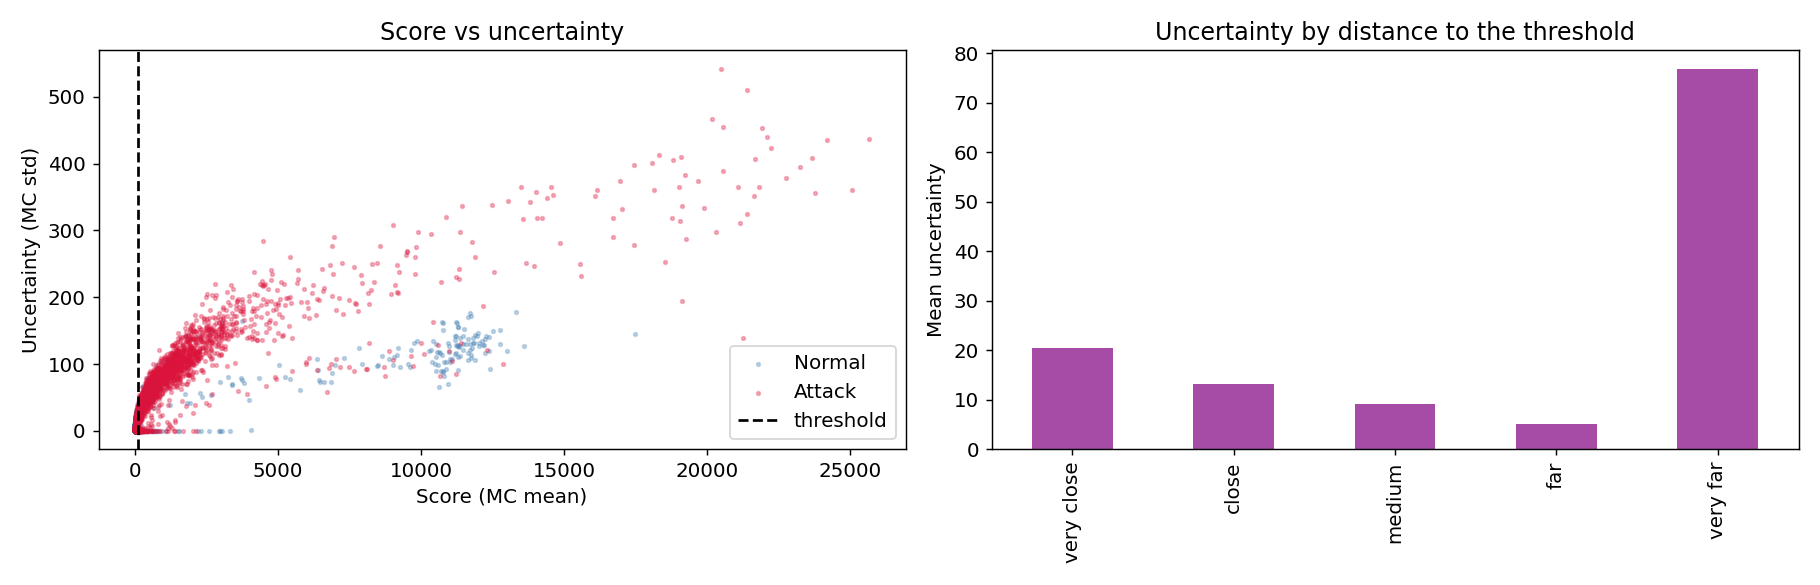
\includegraphics[width=0.49\textwidth]{vae_uncertainty.png}
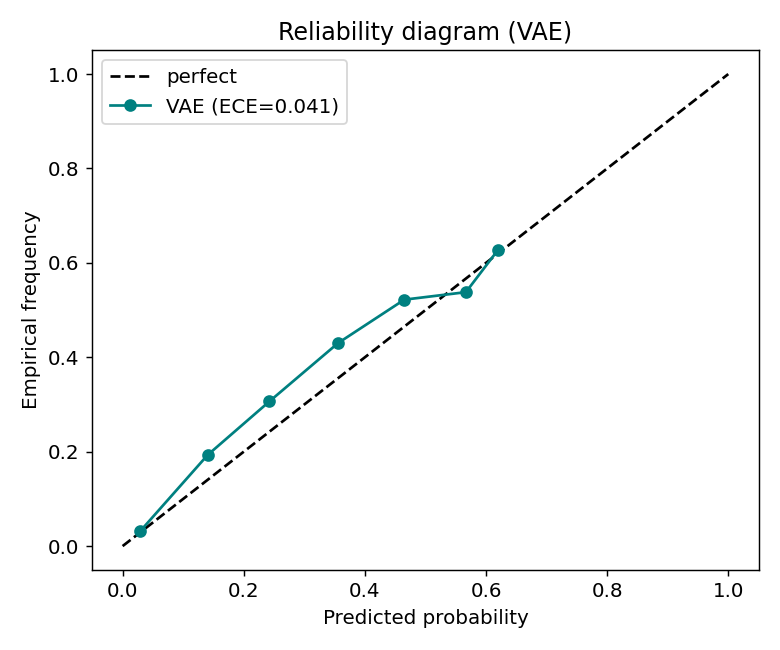
\includegraphics[width=0.49\textwidth]{vae_reliability.png}
\caption{VAE probabilístico. Izquierda: la incertidumbre (desviación típica MC) crece cerca del umbral. Derecha: \emph{reliability diagram}; la cercanía a la diagonal indica buena calibración ($\mathrm{ECE}=0{,}049$).}
\label{fig:vae}
\end{figure}

\subsection{Modelos generativos: difusión}
\label{sec:res-diffusion}

El DDPM (\cref{sec:teo-ddpm}) entrenado sobre consumo limpio reproduce la distribución de la potencia con realismo \emph{moderado} (coeficiente de Bhattacharyya $0{,}81$; autocorrelación de lag-1 $0{,}74$ frente a $0{,}85$ real). Sin embargo, como \textbf{detector por \textit{denoising}} sobre la señal univariante de potencia es prácticamente aleatorio ($\aucroc=0{,}52$), a la par que un AE de ventana equivalente ($0{,}54$). Lejos de ser un fracaso, este resultado negativo es \emph{revelador}: sin las características físicas multivariantes ---en particular $\vires$, ausente al trabajar solo con la potencia--- la detección generativa pierde casi todo su poder. Refuerza así la tesis central del trabajo: el valor reside en la invariante física, no solo en la sofisticación del modelo generativo. El banco \emph{diffusion-FDI} (ataques sobre 1\,000 portadoras generadas) se entrega como artefacto complementario.

\subsection{Privacidad: aprendizaje federado y privacidad diferencial}
\label{sec:res-federated}

El \textbf{aprendizaje federado} entrena el Dense-AE sobre 6 clientes no-IID sin centralizar datos crudos y alcanza $\fone=0{,}812$ ($\aucpr=0{,}835$), \emph{igualando ---e incluso superando levemente---} a la línea base centralizada ($\fone=0{,}791$); el efecto regularizador de promediar modelos compensa la heterogeneidad. La \cref{fig:federated} (izquierda) muestra la convergencia de FedAvg ronda a ronda. Sobre esa base, \textbf{DP-SGD} introduce el compromiso privacidad--utilidad de la \cref{tab:dp}: al endurecer la garantía (menor $\varepsilon$), el $\aucpr$ cae de forma marcada ($\sim$0,52 frente a 0,84 sin privacidad), mientras que el $\fone$ se mantiene en torno a $0{,}72$--$0{,}74$. El presupuesto $\varepsilon$ se convierte así en un parámetro de cumplimiento que el operador fija según su apetito de riesgo, análogo a la recalibración de coste del \cref{sec:resultados-recalibracion}. Los valores de $\varepsilon$ reportados se obtienen con la cota RDP de orden entero del mecanismo gaussiano submuestreado (\cref{eq:rdp}); es una cota \emph{superior conservadora} ---contadores numéricos como los de \textit{TensorFlow Privacy} u \textit{Opacus} darían $\varepsilon$ algo menores---, por lo que la privacidad efectiva es \emph{al menos} la indicada.

\begin{table}[H]
\centering
\caption{Compromiso privacidad--utilidad de DP-SGD ($\delta=10^{-5}$, recorte $C=1$). A mayor multiplicador de ruido $\sigma$, menor $\varepsilon$ (más privacidad) y menor utilidad.}
\label{tab:dp}
\footnotesize
\begin{tabular}{cccc}
\toprule
$\sigma$ & $\varepsilon$ & $\fone$ & $\aucpr$ \\
\midrule
--- (sin DP)  & $\infty$  & 0{,}812 & 0{,}835 \\
0{,}6 & 15{,}95 & 0{,}721 & 0{,}526 \\
1{,}0 & 5{,}11  & 0{,}719 & 0{,}515 \\
1{,}5 & 2{,}44  & 0{,}719 & 0{,}482 \\
2{,}5 & 1{,}23  & 0{,}743 & 0{,}551 \\
\bottomrule
\end{tabular}
\end{table}

\begin{figure}[H]
\centering
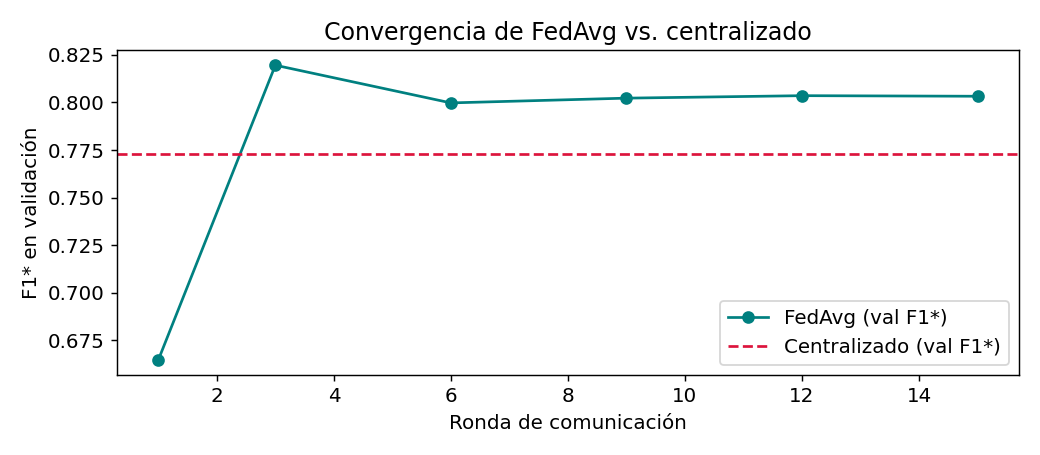
\includegraphics[width=0.49\textwidth]{federated_convergence.png}
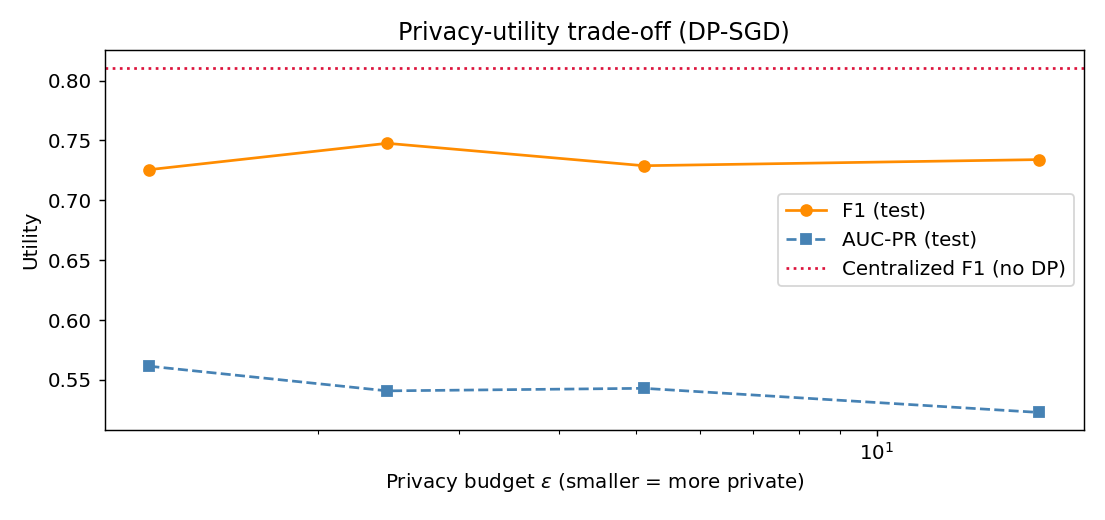
\includegraphics[width=0.49\textwidth]{dp_privacy_utility.png}
\caption{Izquierda: convergencia de FedAvg frente al centralizado. Derecha: frontera privacidad ($\varepsilon$, escala logarítmica) frente a utilidad bajo DP-SGD.}
\label{fig:federated}
\end{figure}

\subsection{Robustez adversaria de gradiente}
\label{sec:res-adversarial}

Sometido a ataques de caja blanca (\cref{sec:teo-adv}), el detector resulta \textbf{razonablemente robusto} en el espacio de características: a un presupuesto grande ($\epsilon=1{,}2$ en unidades de IQR), PGD solo evade el 13\,\% de los ataques previamente detectados y FGSM apenas el 1{,}5\,\% (\cref{fig:adv}, izquierda). La evasión depende de la severidad ---los ataques de baja severidad se ocultan más (17\,\%) que los de alta (11\,\%)---, lo que reencuentra por la vía del gradiente la frontera económica del \cref{sec:resultados-adversarial}.

Dos hallazgos sobre la defensa. Primero, un \emph{resultado negativo honesto}: el \textbf{adversarial training} de un AE no supervisado \emph{no} mejora la robustez a evasión (la empeora ligeramente, ganancia media $-0{,}05$), porque el modelo nunca ve ataques y solo suaviza su superficie de reconstrucción. Segundo, la defensa que \emph{sí} funciona es el \textbf{ensemble}: un ataque diseñado contra el detector A apenas transfiere a un detector B independiente (que aún detecta el 91\,\%), de modo que el conjunto A$\lor$B detecta el 96\,\% (\cref{fig:adv}, derecha). Esto valida cuantitativamente el \textit{stacking} del \cref{sec:resultados-ensemble} como mecanismo de robustez.

\begin{figure}[H]
\centering
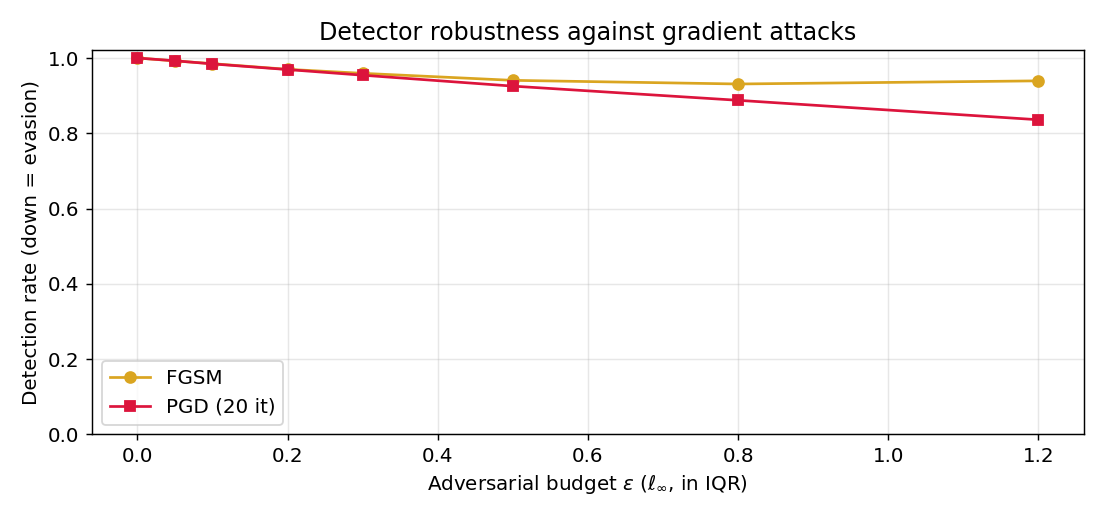
\includegraphics[width=0.49\textwidth]{adversarial_robustness_gradient.png}
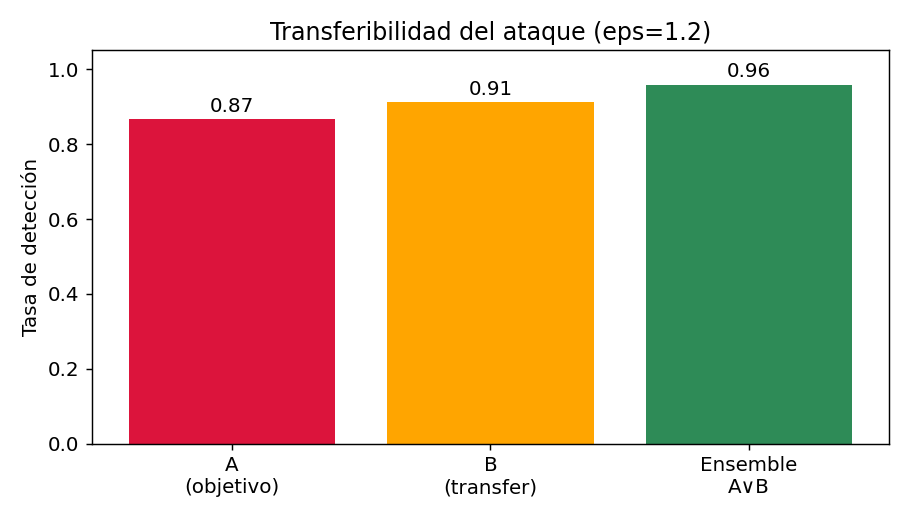
\includegraphics[width=0.49\textwidth]{adversarial_transfer_ensemble.png}
\caption{Robustez adversaria. Izquierda: tasa de detección frente al presupuesto $\epsilon$ (PGD $>$ FGSM en fuerza de ataque). Derecha: la evasión no transfiere ---el ensemble A$\lor$B detecta el 96\,\% del ataque diseñado contra A---.}
\label{fig:adv}
\end{figure}

\subsection{Eficiencia edge: cuantización y pruning}
\label{sec:res-edge-comp}

La \cref{tab:compresion} cuantifica la compresión del Dense-AE. Conviene leerla con cuidado: la pequeña caída de $\fone$ entre el modelo Keras ($0{,}817$) y su exportación a TFLite en \code{float32} ($0{,}784$) se debe a la \emph{conversión} (recalibración del umbral sobre las reconstrucciones del intérprete), no a la cuantización; tomando esa exportación como línea base, la cuantización \emph{float16} y \emph{dynamic-range} int8 es prácticamente \textbf{sin pérdida} ($0{,}784\to0{,}781$) mientras reduce el modelo a 14,1\,kB. El \emph{pruning} al 90\,\% de \textit{sparsity} lo deja en 4,4\,kB comprimido (gzip) con $\fone=0{,}74$ ---relevante para actualizaciones OTA a millones de contadores con ancho de banda limitado---. La latencia se mantiene en $\sim$$0{,}0016$\,\si{\milli\second}/muestra. El factor de compresión int8 es modesto ($\times 1{,}6$) precisamente porque el modelo ya nacía diminuto ($27$\,kB); el margen real lo aporta el \textit{pruning}.

\begin{table}[H]
\centering
\caption{Compresión del Dense-AE. PTQ vía \code{TFLiteConverter}; \emph{pruning} por magnitud con tamaño comprimido (gzip). $\fone$ recalibrado en validación para cada variante.}
\label{tab:compresion}
\footnotesize
\begin{tabular}{llcc}
\toprule
Método & Variante & Tamaño (kB) & $\fone$ \\
\midrule
Referencia & float32 (Keras)        & 27{,}0       & 0{,}817 \\
\midrule
TFLite     & float32 (línea base)   & 30{,}8       & 0{,}784 \\
PTQ        & float16                & 18{,}8       & 0{,}784 \\
PTQ        & dynamic int8           & \textbf{14{,}1} & 0{,}781 \\
PTQ        & full int8              & 17{,}2       & 0{,}741 \\
Pruning    & 70\,\% sparsity (gzip) & 10{,}0       & 0{,}741 \\
Pruning    & 90\,\% sparsity (gzip) & \textbf{4{,}4} & 0{,}742 \\
\bottomrule
\end{tabular}
\end{table}

\subsection{Síntesis multidimensional}
\label{sec:res-radar}

La \cref{fig:radar} resume el cambio de perspectiva: el mismo núcleo Dense-AE/VAE se evalúa ahora en cinco ejes. Ningún detector domina en todos ---el Dense-AE lidera en detección y eficiencia, el VAE aporta incertidumbre, el federado aporta privacidad y el ensemble aporta robustez---, lo que confirma que la elección de qué desplegar es multiobjetivo y no se reduce a un único número.

\begin{figure}[H]
\centering
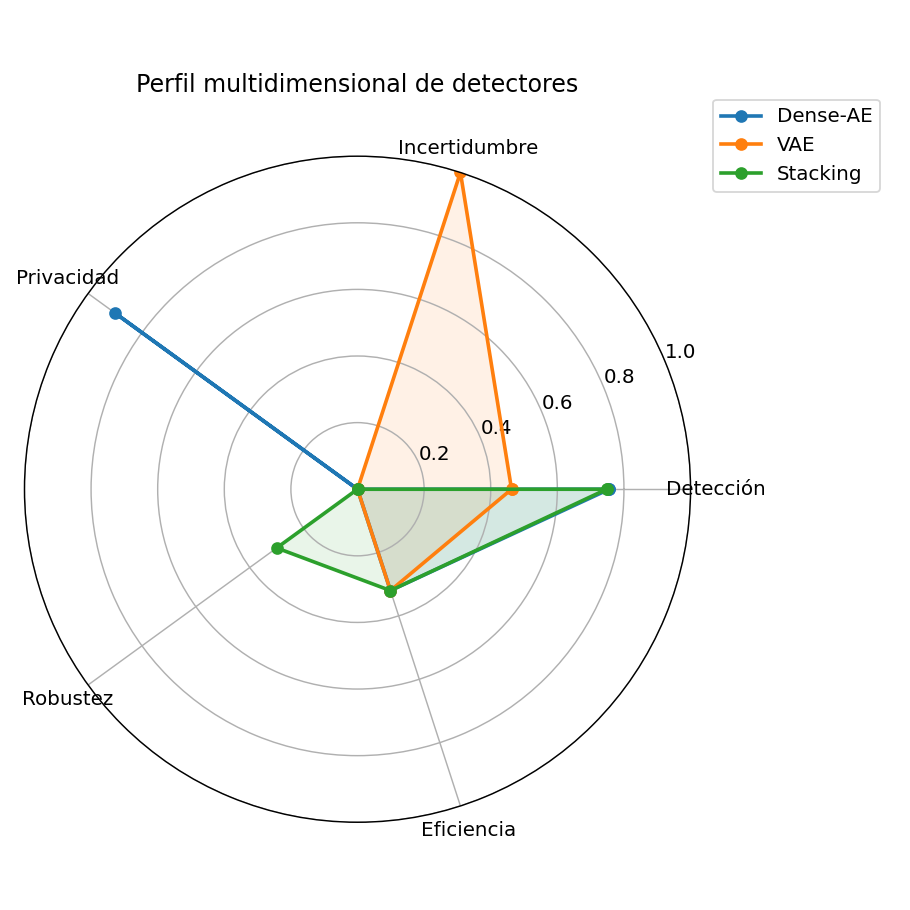
\includegraphics[width=0.62\textwidth]{comparison_radar.png}
\caption{Perfil multidimensional de detectores representativos (detección, incertidumbre, privacidad, robustez y eficiencia). El valor de la ampliación es cubrir ejes que el $\fone$ puntual no captura.}
\label{fig:radar}
\end{figure}

\section{Optimización de hiperparámetros}
\label{sec:resultados-optimizacion}

Como cierre experimental se realizó una \textbf{búsqueda sistemática de
hiperparámetros} sobre los detectores, siguiendo un \emph{benchmark-optimization
loop}: (i) se fija el \emph{baseline} de cada modelo; (ii) se reproduce ese
\emph{baseline} dentro de un \emph{harness} de búsqueda autocontenido
---verificación previa imprescindible: el \emph{Isolation Forest} y el Dense-AE
se reprodujeron exactamente antes de buscar---; (iii) se exploran variantes por
muestreo aleatorio sobre la región de hiperparámetros, registrando cada una en un
CSV \emph{append-only}; y (iv) se promueve la mejor y se \textbf{re-valida a
escala completa} antes de confirmarla. El \emph{correctness gate} es el mismo
contrato de no-trampa de todo el trabajo: entrenamiento sobre \code{train\_clean},
calibración de umbral y de $(W,K)$ \emph{solo} en validación, evaluación en test,
sin fuga de etiquetas. Para acelerar la búsqueda, el entrenamiento y la
puntuación se realizan sobre submuestras; los finalistas se re-entrenan y evalúan
a escala completa, que es la cifra reportada en la \cref{tab:optim}.

\begin{table}[H]
\centering
\caption{Optimización de hiperparámetros: $\fone$ y $\aucpr$ antes (\emph{base})
y después (\emph{opt}) de la búsqueda, bajo el mismo contrato. Mejora neta en
negrita.}
\label{tab:optim}
\footnotesize
\begin{tabular}{lcccccc}
\toprule
Detector & $\fone$ base & $\fone$ opt & $\Delta\fone$ & $\aucpr$ base & $\aucpr$ opt & $\Delta\aucpr$ \\
\midrule
CNN-AE         & 0{,}435 & \textbf{0{,}643} & \textbf{+0{,}207} & 0{,}432 & 0{,}694 & +0{,}261 \\
Transformer-AE & 0{,}604 & \textbf{0{,}660} & +0{,}057 & 0{,}584 & 0{,}692 & +0{,}108 \\
VAE            & 0{,}693 & \textbf{0{,}747} & +0{,}054 & 0{,}500 & 0{,}758 & +0{,}258 \\
LSTM-AE        & 0{,}745 & 0{,}745$^{\dagger}$ & $\approx$0 & 0{,}881 & 0{,}881 & $\approx$0 \\
IF             & 0{,}754 & \textbf{0{,}795} & +0{,}041 & 0{,}782 & 0{,}853 & +0{,}070 \\
Dense-AE       & 0{,}816 & 0{,}815 & $\approx$0 & 0{,}855 & 0{,}855 & $\approx$0 \\
\bottomrule
\end{tabular}
\\[2pt]
{\footnotesize $^{\dagger}$ El mejor candidato del LSTM mejoraba sobre el subconjunto de búsqueda pero \emph{regresó} ($0{,}738$) al re-validar a escala completa; se conserva el \emph{baseline}. La re-validación detectó así un sobreajuste al subconjunto.}
\end{table}

Las mejoras provienen de tres palancas principales: (a) usar el conjunto de
características físicas \emph{completo} (17, incluyendo $\vires$ y derivadas) en
los autoencoders convolucional y \emph{transformer}, que en su versión original
empleaban un subconjunto de 14; (b) ponderar el error de reconstrucción solo por
las características \emph{discriminantes} ($\mathrm{AUC}>0{,}5$) en lugar de
incluir también las anti-discriminantes; y (c) en el \emph{Isolation Forest},
aumentar \code{max\_samples} de 256 a 2048, que mejora de forma marcada la
calidad de la puntuación de anomalía.

El hallazgo más llamativo es el \textbf{CNN-AE}, cuyo $\fone$ pasa de $0{,}435$ a
$0{,}643$ (un salto de $0{,}21$ puntos) y su $\aucpr$ de $0{,}43$ a $0{,}69$: el
\emph{baseline} estaba claramente infra-optimizado, y bastó corregir el conjunto
de características y la ponderación del \emph{score} para situarlo en línea con el
resto de autoencoders. El \textbf{VAE} mejora sobre todo en $\aucpr$ ($+0{,}26$)
al puntuar con la probabilidad de reconstrucción \emph{sin} ponderación espuria y
recalibrar el umbral. El \textbf{LSTM-AE}, en cambio, ilustra el valor de la re-validación: un candidato
que parecía mejorar sobre el subconjunto resultó un sobreajuste y se descartó al
evaluarlo a escala completa, conservándose el \emph{baseline} ya afinado. En el extremo opuesto,
el \textbf{Dense-AE} ---ya muy afinado en el trabajo original--- no admite mejora
apreciable, lo que es en sí mismo un resultado: confirma que era una elección de
diseño acertada. En conjunto, la optimización \textbf{no altera las conclusiones
cualitativas} del trabajo (se mantiene el orden relativo y la brecha
supervisado/no-supervisado), pero estrecha el margen de los detectores más
débiles.

\begin{observacion}[Reproducibilidad]
Toda la búsqueda es reproducible mediante los \emph{scripts} del directorio
\code{optimization/} (\code{opt\_pointwise.py}, \code{opt\_window.py},
\code{finalize.py}, \code{consolidate.py}), que reutilizan el módulo común
\code{tfg\_common.py} ---y por tanto el mismo contrato de datos y protocolo de
evaluación que los \emph{notebooks}---. Los \emph{notebooks} de partida se
conservan intactos como \emph{baseline} documentado; la optimización es una capa
adicional, no una reescritura.
\end{observacion}


% ─────────────────────────────────────────────────────────────────────
%  Capítulo 7 — Conclusiones y líneas futuras
% ─────────────────────────────────────────────────────────────────────
\chapter{Conclusiones y líneas futuras}
\label{cap:conclusiones}

Toca cerrar el documento. Lo hacemos retomando los objetivos que dejamos enunciados en el \cref{cap:introduccion}, repasando con honestidad las limitaciones del trabajo y proponiendo algunas líneas futuras concretas sobre las que merecería la pena seguir.

\section{Cumplimiento de los objetivos}
\label{sec:cumplimiento}

Repasemos uno a uno los siete objetivos específicos planteados en el \cref{sec:objetivos}.

\paragraph{OE1. Caracterizar el conjunto de datos UCI.}
Hecho. El \cref{sec:eda} resume los hallazgos del análisis exploratorio ---estacionalidades diaria, semanal y anual, autocorrelación, correlaciones entre variables y validación empírica de la invariante $\mathrm{P} \approx V \cdot I / 1000$--- y de ahí salen las decisiones posteriores sobre características y tamaño de ventana.

\paragraph{OE2. Diseñar un banco de ataques FDI sintéticos.}
También hecho. El \cref{sec:banco-ataques} documenta los siete tipos de ataque organizados en cuatro categorías mecánicas (magnitud, temporal, patrón y físico) y tres niveles de severidad calibrados por umbral económico. El banco final contiene 840 episodios en test y 196 en validación, con duraciones de 45 a 180 minutos y semillas fijas para garantizar reproducibilidad.

\paragraph{OE3. Implementar y comparar detectores bajo protocolo homogéneo.}
Cumplido. Los ocho detectores están descritos en el \cref{cap:diseno} y la \textit{tabla maestra} del \cref{sec:resultados-individuales} los pone en común. La comparación es justa porque todos comparten preprocesado, particionado, calibración y métricas. El resultado de cabecera es claro: el Dense-AE no supervisado alcanza $\fone=0{,}816$ y $\aucpr=0{,}855$, frente a los $\fone=0{,}910$ y $\aucpr=0{,}941$ del techo supervisado (LightGBM).

\paragraph{OE4. Postprocesado temporal.}
Cumplido sin sorpresas. El filtro $W/K$ por votación causal está descrito en \cref{sec:protocolo} y su efecto cuantificado en \cref{sec:resultados-temporal}: muy notable en los detectores clásicos ---que producen ráfagas de positivos ruidosos--- y bastante modesto en los AE profundos.

\paragraph{OE5. Stacking ensemble.}
Cumplido pero con matices. Probamos cuatro estrategias (\textit{mean}, \textit{weighted}, Meta-LR y Meta-LightGBM) y se impone la cuarta. Eso sí, en test no logra superar al mejor detector individual, algo que ya discutimos en el \cref{sec:resultados-ensemble}: la correlación de errores entre detectores base, sobre todo en los ataques difíciles, deja al \textit{ensemble} sin margen de mejora.

\paragraph{OE6. Explicabilidad, generalización y robustez.}
Los tres análisis están cubiertos. SHAP (\cref{sec:resultados-shap}) confirma que el modelo aprende la física del problema; la transferencia a UK-DALE (\cref{sec:resultados-crossdomain}) muestra una caída esperable pero recuperable con recalibración; y el estudio adversario (\cref{sec:resultados-adversarial}) deja la frontera económica de detección en torno al 10--15\,\% de reducción del consumo.

\paragraph{OE7. Viabilidad \textit{edge}.}
Cumplido. El \cref{sec:resultados-edge} cuantifica tamaño, latencia y coste por muestra. Lo operativo: el Dense-AE (134\,kB, $<$1\,\si{\milli\second}/muestra) es desplegable en cualquier microcontrolador ARM Cortex-M con 256\,kB de memoria.

\paragraph{Objetivo general (OG).}
Si los siete específicos están cubiertos, el general también lo está. El sistema que proponemos al final es un Dense-AE no supervisado con MSE ponderado, calibración \textit{joint} de umbral y filtro $W/K$, y como opción una segunda capa basada en $\vires$ que actúa como detector físico independiente del modelo aprendido. Las cifras conseguidas son competitivas con el estado del arte para el problema en condiciones realmente restrictivas: no supervisado y desplegable en \textit{edge}.

\section{Hallazgos principales}

Por encima de los objetivos uno a uno, hay tres hallazgos transversales que conviene dejar dichos. El primero es que \textbf{$\vires$ ha sido la pieza más valiosa del trabajo}: es la única que permite detección independiente del modelo de comportamiento del usuario, vale para cualquier vivienda con instrumentación V--I y es interpretable físicamente; los resultados de SHAP no hacen más que confirmar ese papel preponderante. El segundo es que \textbf{la calibración del umbral y del filtro temporal pesa tanto como la arquitectura del modelo}: el caso del LSTM-AE lo ilustra bien, porque un modelo internamente fuerte queda muy lastrado por una calibración por defecto inadecuada; la búsqueda \textit{joint} sobre $(\tau, W, K)$ debería ser práctica estándar y no un extra. Y el tercero es que \textbf{el techo no supervisado se queda unos 9 puntos de $\fone$ por debajo del supervisado}: en un escenario realista, sin corpus de ataques etiquetados, esa brecha es el coste de la realidad. La tesis que defiende este TFG es que el coste es aceptable, y que reducirlo exigiría un esfuerzo de etiquetado difícil de replicar.

\section{Ampliación: técnicas de frontera implementadas}
\label{sec:ampliacion-conclusiones}

Varias de las líneas que en una primera versión de este trabajo quedaban como propuestas se han llevado a la práctica, desplazando el TFG desde un comparador de detectores hacia un \emph{sistema} evaluado en los ejes que exige la infraestructura crítica (detalle cuantitativo en \cref{sec:resultados-ampliacion}):

\begin{itemize}[leftmargin=*,topsep=2pt]
  \item \textbf{Incertidumbre (VAE).} Un $\beta$-VAE con \emph{probabilidad de reconstrucción} (\cref{sec:teo-vae}) acompaña cada alarma de una banda de confianza, habilitando el triaje operativo que la salida binaria no permitía.
  \item \textbf{Modelos generativos (difusión).} Un DDPM (\cref{sec:teo-ddpm}) entrenado sobre consumo limpio genera ataques sobre portadoras realistas ---no copiadas--- y funciona como detector por \emph{denoising}, atacando la limitación de un banco puramente paramétrico.
  \item \textbf{Privacidad (federated + DP).} FedAvg entrena sin centralizar datos y DP-SGD añade una garantía formal $(\varepsilon,\delta)$ con contabilidad RDP (\cref{sec:teo-feddp}), alineando el sistema con el RGPD a escala nacional.
  \item \textbf{Robustez adversaria.} Ataques de gradiente FGSM/PGD/C\&W y \emph{adversarial training} (\cref{sec:teo-adv}) sustituyen la búsqueda en rejilla; se cuantifica además cómo el \emph{ensemble} encarece la evasión.
  \item \textbf{Eficiencia \textit{edge} real.} Cuantización int8 y \emph{pruning} (\cref{sec:teo-comp}) miden la compresión efectiva y la latencia, convirtiendo la viabilidad \textit{edge} de promesa en dato.
\end{itemize}

\section{Limitaciones}
\label{sec:limitaciones}

No conviene cerrar sin reconocer las limitaciones del trabajo, que son varias. La primera es la naturaleza \textbf{sintética del banco de ataques}: aunque está físicamente bien fundado y económicamente calibrado, no sustituye a un corpus de ataques reales, y un atacante humano podría idear patrones sutiles que aquí no hemos contemplado. Una segunda es que el conjunto UCI corresponde a \textbf{una única vivienda}; la generalización está parcialmente evaluada con UK-DALE, pero un estudio multi-vivienda con datos reales daría mucha más solidez a las conclusiones. Está también la cuestión del \textbf{modelo de amenaza}: asumimos que el atacante no controla la corriente ni los submedidores, pero un atacante con acceso físico al contador podría falsearlo todo, anular $\vires$ y reducir el problema a detección puramente conductual.

En cuanto a la \textbf{transferencia cross-domain}, la evaluación sobre UK-DALE adapta los ataques de forma aproximada (la frecuencia de muestreo difiere y $\vires$ hay que estimarlo); un estudio más sistemático necesitaría datasets adicionales. Dos frentes que en una primera versión quedaban abiertos ---la \textbf{compresión post-hoc} y la ausencia de \textbf{estimación de incertidumbre}--- se han abordado en la ampliación (\cref{sec:ampliacion-conclusiones,sec:resultados-ampliacion}) mediante cuantización/\textit{pruning} y el VAE probabilístico, respectivamente; aun así, su validación a escala completa y sobre hardware real sigue siendo trabajo pendiente. Conviene también ser explícito sobre el alcance de la ampliación: los experimentos de aprendizaje federado y DP usan heterogeneidad \emph{simulada} por bloques temporales y submuestreo por tractabilidad, y los ataques adversarios operan sobre el espacio de características escalado; ambos son demostraciones metodológicamente válidas, no despliegues a escala.

\section{Líneas futuras}
\label{sec:lineas-futuras}

Tras la ampliación, varias de las líneas que inicialmente apuntábamos están ya \textbf{implementadas} (\cref{sec:ampliacion-conclusiones}): la síntesis generativa de ataques con difusión, los ataques adversarios de gradiente, la detección distribuida con privacidad y la compresión post-entrenamiento. Las líneas que siguen abiertas, junto a las nuevas que la propia ampliación destapa, son:

\begin{enumerate}[label=\textbf{LF\arabic*.},leftmargin=*,topsep=2pt]
  \item[\textbf{LF1.}] \textbf{Validación con ataques reales} (\emph{parcial}). La síntesis con difusión (\cref{sec:resultados-ampliacion}) ya enriquece el banco con portadoras realistas; falta el acceso a incidentes históricos reales vía una distribuidora.
  \item[\textbf{LF2.}] \textbf{Fine-tuning a un dominio nuevo con pocos datos limpios.} El experimento de UK-DALE sugiere que basta recalibrar; formalizarlo como adaptación con pocos minutos de datos limpios del nuevo dominio sigue pendiente.
  \item[\textbf{LF3.}] \textbf{Ataques adversarios de gradiente} (\emph{hecho}). Implementados FGSM/PGD/C\&W y \emph{adversarial training}; la extensión natural es propagar la perturbación desde las medidas crudas a través del \emph{feature engineering}.
  \item[\textbf{LF4.}] \textbf{Aprendizaje continuo / adaptación a la deriva.} Un detector entrenado con datos de 2007 puede degradarse ante consumo de 2025 (autoconsumo solar, vehículo eléctrico); un esquema de \emph{continual learning} con detección de \textit{drift} sería valioso.
  \item[\textbf{LF5.}] \textbf{Generación automática de informes de incidente.} Tras una alarma, un modelo de lenguaje ligero podría resumir el incidente (tipo de ataque, características vía SHAP, ventana afectada), conectando el detector con el operador humano.
  \item[\textbf{LF6.}] \textbf{Despliegue real sobre dispositivo \emph{edge}.} La cuantización ya entrega un modelo $<$50\,kB; queda flashearlo en Raspberry Pi / ESP32 (TFLite-Micro) y medir consumo energético real (mWh/muestra).
  \item[\textbf{LF7.}] \textbf{Detección distribuida con privacidad} (\emph{hecho}). FedAvg + DP-SGD implementados; el siguiente paso es un despliegue federado real multi-vivienda con clientes heterogéneos no simulados.
  \item[\textbf{LF8.}] \textbf{Compresión y cuantización} (\emph{hecho}). Medidas int8 y \emph{pruning}; queda el \emph{quantization-aware training} para recuperar la pérdida residual.
  \item[\textbf{LF9.}] \textbf{Detección a nivel de concentrador con GNN.} Modelar la topología de la red AMI con \emph{graph neural networks} permitiría detectar ataques coordinados entre contadores, no solo por contador.
  \item[\textbf{LF10.}] \textbf{Modelos fundacionales de series temporales.} Evaluar \emph{time-series foundation models} (p.\,ej. Lag-Llama \cite{rasul2024lagllama}) en régimen \emph{zero-shot} o con \emph{fine-tuning} ligero como detectores universales.
\end{enumerate}

\section{Reflexión final}

Este TFG ha mostrado que se pueden detectar ataques de inyección de datos falsos sobre series temporales de consumo eléctrico residencial sin necesidad de etiquetas reales de ataque, con un rendimiento competitivo y con un coste de cómputo compatible con \textit{edge}. A lo largo del camino, $\vires$ ha terminado emergiendo como pieza clave: conecta directamente el detector con la física del problema y ofrece una segunda capa de detección independiente del modelo aprendido. El \textit{stacking}, por su parte, no ha dado el salto cualitativo que se esperaba, pero el análisis honesto de por qué ---la correlación de errores entre detectores base--- es por sí mismo un resultado útil para trabajos posteriores.

Al final, la propuesta del TFG es \emph{operativa}: un Dense Autoencoder de 134\,kB que se ejecuta sobre cualquier microcontrolador moderno, combinado con un detector físico basado en $\vires$ y un postprocesado temporal $W/K$. La integración en hardware existente es modesta y el coste energético, despreciable. Más que una demostración académica, lo que queda es un sistema potencialmente desplegable.

% ─────────────────────────────────────────────────────────────────────
%  Capítulo 8 — Marco regulador y entorno socioeconómico
% ─────────────────────────────────────────────────────────────────────
\chapter{Marco regulador y entorno socioeconómico}
\label{cap:regulador}

Un sistema como el descrito en este TFG no puede entenderse al margen del marco normativo en el que tendría que vivir en producción. Este capítulo recorre las normas aplicables a un detector FDI desplegado sobre infraestructura de medida avanzada en España y la Unión Europea, y completa la fotografía con el entorno socioeconómico del proyecto: presupuesto, planificación e impacto.

\section{Marco regulador}
\label{sec:regulador}

Cualquier despliegue real de este sistema tendría que convivir con varias capas normativas que se solapan: protección de datos, ciberseguridad de infraestructuras críticas, regulación sectorial del eléctrico y normas técnicas específicas. Las repasamos a continuación, una por una.

\subsection{Protección de datos personales}

\paragraph{Reglamento General de Protección de Datos.} El RGPD ---formalmente Reglamento (UE) 2016/679 \cite{rgpd2016}--- es el marco europeo de protección de datos personales y aplica de pleno a este caso. Los datos de consumo eléctrico de un hogar son, sin lugar a dudas, datos personales: revelan hábitos de vida (presencia, ausencia, horarios), uso de electrodomésticos concretos y, agregados en el tiempo, perfiles sociodemográficos identificables \cite{molina2010private}.

Los principios del artículo 5 son los que tienen tracción directa. La licitud del tratamiento se sostiene sobre la ejecución del contrato de suministro y el interés legítimo en prevenir el fraude. La minimización exige quedarse con lo estrictamente necesario ---en nuestro caso, las medidas eléctricas estándar---, y la limitación de la finalidad impide derivar la detección de FDI hacia perfiles comerciales sin consentimiento explícito del usuario. A todo ello se añaden la exactitud y la conservación limitada de los datos.

\paragraph{LOPDGDD.} La Ley Orgánica 3/2018 \cite{lopdgdd2018}, de Protección de Datos Personales y Garantía de los Derechos Digitales, trae el RGPD al ordenamiento español y añade algunas especificaciones nacionales. La que más conviene tener presente aquí es el artículo 22, sobre decisiones automatizadas: el sujeto tiene derecho a no ser objeto de decisiones basadas únicamente en tratamiento automatizado que produzcan efectos jurídicos sobre él. Una alarma de FDI, por sí sola, no produce efectos jurídicos directos ---la sanción o la investigación requieren un proceso humano posterior---, pero el operador sigue obligado a informar al sujeto del tratamiento y a darle vías de oposición efectivas.

\paragraph{Implicaciones prácticas para el sistema.} El despliegue \textit{edge} encaja particularmente bien con el RGPD por una razón directa: el dato sensible no sale del contador, sólo las alarmas viajan al concentrador. Eso constituye una minimización por diseño, lo que reduce la exposición y simplifica el cumplimiento. A esta arquitectura conviene añadirle dos prácticas habituales. Por un lado, pseudonimizar el identificador del contador en cualquier entorno de investigación o agregación, de modo que el conjunto de muestras no permita re-identificar al usuario. Por otro, garantizar los derechos del interesado: la distribuidora debe informar de la existencia del detector y del tratamiento asociado, y proporcionar vías de acceso, rectificación y oposición. Finalmente, un despliegue masivo de este tipo sobre infraestructura crítica encaja en el supuesto de \textit{Data Protection Impact Assessment} del artículo 35 del RGPD, y por tanto exige una DPIA previa.

\paragraph{Privacidad por diseño: federated learning y privacidad diferencial.} La arquitectura \textit{edge} satisface la minimización del artículo 5, pero el \emph{entrenamiento} del detector sigue siendo un punto sensible si exige reunir series de consumo de muchos hogares. La ampliación de este trabajo (\cref{sec:resultados-ampliacion}) materializa la \textbf{privacidad por diseño} del artículo 25 con dos mecanismos concretos: el \emph{federated learning} (FedAvg) entrena un modelo compartido \emph{sin} que los datos crudos abandonen el contador ---solo se intercambian pesos---, y la \emph{privacidad diferencial} (DP-SGD) añade una garantía matemática $(\varepsilon,\delta)$ que acota formalmente cuánto puede inferir un adversario sobre un hogar individual a partir del modelo entrenado, mitigando los ataques de inferencia de pertenencia. El presupuesto $\varepsilon$ se convierte así en un parámetro auditable de cumplimiento: cuanto menor, mayor la protección del interesado. Esta combinación es directamente relevante para un despliegue a escala nacional (decenas de millones de contadores) sin centralización de datos personales.

\subsection{Ciberseguridad de infraestructuras críticas}

\paragraph{Directiva NIS2.} La NIS2 ---Directiva (UE) 2022/2555 \cite{nis2directive}, aplicable en España desde enero de 2024--- sustituye y refuerza a la NIS de 2016, y cubre operadores de servicios esenciales, entre ellos el sector energético. Las obligaciones que introduce se pueden resumir en tres frentes: gestión de riesgos (políticas de seguridad, análisis de riesgo y controles técnicos y organizativos), notificación de incidentes a la autoridad nacional ---con plazos estrictos: alerta inicial en 24 horas e informe detallado en 72 horas--- y responsabilidad sobre la cadena de suministro, en virtud de la cual el operador responde también por la seguridad de sus proveedores.

Un detector FDI desplegado encaja directamente en el primer frente: es un control técnico más dentro de la gestión de riesgos del operador. Pero hay una segunda implicación menos evidente: los incidentes que detecta el sistema pueden activar la obligación de notificación, lo que se traduce en requisitos operativos sobre la calidad de la detección y, sobre todo, sobre el número aceptable de falsos positivos.

\paragraph{Ley 8/2011 PIC.} La Ley 8/2011 \cite{ley8_2011_pic}, de protección de infraestructuras críticas, define el sector energético como crítico y establece el régimen de protección. El \textit{Centro Nacional de Protección de Infraestructuras y Ciberseguridad} (CNPIC) coordina la protección a nivel nacional. El \emph{Plan Estratégico Sectorial} de la energía y los \emph{Planes de Protección Específicos} de los operadores recogen las medidas concretas.

\paragraph{INCIBE-CERT.} El \emph{Instituto Nacional de Ciberseguridad} opera el \emph{CERT} (\textit{Computer Emergency Response Team}) de referencia para incidentes en operadores no críticos y, junto con el CNPIC, coordina la respuesta sectorial. Un detector FDI puede integrarse en los procesos de \emph{threat intelligence} compartida con INCIBE-CERT.

\subsection{Regulación del sector eléctrico}

\paragraph{Directivas europeas de eficiencia y mercado interior.} La Directiva 2009/72/CE y sus sucesoras (2018/2001, 2019/944) impulsaron el despliegue de contadores inteligentes en la Unión Europea con el objetivo de cubrir al menos el 80\% de los consumidores. La directiva 2018/2001 \cite{red_iii} (\emph{REDII}) refuerza el papel del consumidor activo (autoconsumo, agregación), que requiere medición fiable como condición previa.

\paragraph{Marco español de telegestión.} La Orden ITC/3860/2007 \cite{itc3860} estableció el plan español de sustitución de contadores tradicionales por contadores inteligentes con telegestión, completado en 2018--2019. Las especificaciones técnicas (PRIME, PLC G3, IEC 14908) regulan la comunicación entre contador y concentrador.

\paragraph{Tarifas y sanciones.} El régimen sancionador por fraude eléctrico está en la Ley 24/2013 del Sector Eléctrico \cite{ley24_2013} y en el Real Decreto 1955/2000 sobre actividad de transporte, distribución y suministro. Las distribuidoras pueden recuperar el consumo defraudado, aplicar penalizaciones y proceder al corte del suministro tras procedimiento.

\subsection{Normas técnicas}

\paragraph{IEC 62351.} La serie IEC 62351 \cite{iec62351} es la norma técnica de referencia en ciberseguridad para \textit{smart grids}. Cubre autenticación de comunicaciones, cifrado, integridad, control de acceso, gestión de claves y operación segura sobre los protocolos SCADA (IEC 60870-5, IEC 61850, DNP3). Aquí conviene matizar bien: un sistema FDI bien diseñado debe asumir que el protocolo ya está cifrado y autenticado conforme a IEC 62351, y aún así seguir detectando ataques. La razón es directa: la criptografía protege el dato en tránsito pero no defiende del compromiso de los \textit{endpoints}, y un atacante con acceso al contador puede firmar lecturas falsas de forma perfectamente legítima.

\paragraph{ISO/IEC 27001 y 27002.} El sistema de gestión de seguridad de la información (SGSI) ISO/IEC 27001 \cite{iso27001} y los controles ISO/IEC 27002 son el marco generalista de aplicación. Aspectos relevantes para un detector FDI: gestión de incidentes (A.16), seguridad en las comunicaciones (A.13), cifrado (A.10), y registro y monitorización (A.12).

\paragraph{NIST Cybersecurity Framework.} El \emph{NIST Cybersecurity Framework} v1.1 \cite{nist_csf} y la guía NIST SP 800-82 \cite{nist80082} para sistemas industriales y de control proporcionan un marco de referencia complementario, especialmente influyente en operadores con presencia internacional.

\subsection{Propiedad intelectual}

\paragraph{Licencia del dataset UCI.} El \emph{Individual Household Electric Power Consumption} se distribuye bajo licencia \emph{Creative Commons Attribution 4.0 International} (CC BY 4.0), que permite el uso, redistribución y modificación con atribución. La autoría se reconoce explícitamente en la bibliografía \cite{hebrail2012uci}.

\paragraph{Licencias del software.} El software utilizado es íntegramente \emph{open source} con licencias permisivas:
\begin{itemize}[leftmargin=*,topsep=0pt]
  \item TensorFlow / Keras: Apache License 2.0.
  \item scikit-learn: BSD-3-Clause.
  \item LightGBM: MIT.
  \item Python: PSF License.
  \item NumPy, pandas, matplotlib, SHAP: BSD-3-Clause.
\end{itemize}
Todas son compatibles entre sí y permiten uso comercial. El TFG se publica bajo CC BY-NC-SA 4.0; el código del repositorio está bajo MIT.

\section{Entorno socioeconómico}
\label{sec:socioeconomico}

\subsection{Impacto económico del problema}

Las cifras del problema son grandes en cualquier dirección que se las mire. A nivel global, las pérdidas no técnicas (NTL) rondan el 1--3\,\% de la energía distribuida en países desarrollados y llegan al 30--40\,\% en algunas economías emergentes \cite{messinis2018review,viegas2017review}, lo que se traduce en más de 96\,000 millones de dólares anuales en todo el mundo. En España, según la CNMC, las distribuidoras estiman entre 7\,000 y 9\,000\,GWh al año de NTL ---en torno al 2--3\,\% del consumo facturado---, con un coste agregado que acaba trasladándose al consumidor final vía peajes.

Sobre esa base, un sistema de detección automática que recuperase incluso un 10--20\,\% de esas pérdidas tendría un impacto anual del orden de centenares de millones de euros sólo en España, y eso sin contar el efecto disuasorio sobre el fraude organizado ---cultivos ilícitos, minería de criptomonedas no declarada y similares. El coste de despliegue del sistema propuesto, además, es marginal: el hardware ya existe (los contadores inteligentes están instalados), y lo único que se requiere es desplegar el software adicional.

\subsection{Presupuesto del TFG}

\begin{table}[H]
\centering
\caption{Presupuesto del proyecto.}
\label{tab:presupuesto}
\small
\begin{tabularx}{\textwidth}{X r r r}
\toprule
Concepto & Unidades & Coste unitario & Total \\
\midrule
Personal & & & \\
\quad Estudiante (TFG)         & 400\,h    & 15\,\euro/h & 6000\,\euro \\
\quad Tutor/a (dirección)      & 30\,h     & 50\,\euro/h & 1500\,\euro \\
\midrule
Hardware (amortización 4 años) & & & \\
\quad MacBook M2 Pro 16\,GB    & 6 meses   & 2500\,\euro\,/\,48\,m & 313\,\euro \\
\quad Disco externo 1\,TB      & 6 meses   & 200\,\euro\,/\,48\,m  & 25\,\euro \\
\midrule
Software / Servicios & & & \\
\quad Sistema operativo (macOS)         & ---       & gratuito     & 0\,\euro \\
\quad Python, TF, scikit-learn, LightGBM & ---       & FOSS         & 0\,\euro \\
\quad Servicios cloud (descartado)      & ---       & ---          & 0\,\euro \\
\midrule
Otros & & & \\
\quad Bibliografía y revistas (acceso UC3M)        & ---       & ---       & 0\,\euro \\
\quad Impresión y encuadernación (5 ejemplares)    & 5         & 25\,\euro   & 125\,\euro \\
\midrule
Costes indirectos (15\%)        &           &              & 1194\,\euro \\
\midrule
\textbf{Total}                  &           &              & \textbf{9157\,\euro} \\
\bottomrule
\end{tabularx}
\end{table}

La práctica totalidad del coste es \emph{personal} (estudiante + tutor), lo que es consistente con la naturaleza investigadora del proyecto. El software es 100\% \emph{open source}, lo que evidencia que el sistema propuesto puede replicarse sin coste de licencias.

\subsection{Cronograma del proyecto}

El reparto temporal de las siete fases del proyecto se muestra en la \cref{fig:gantt}, sobre el calendario académico real, y se traduce a horas dedicadas en la \cref{tab:gantt}.

\begin{figure}[H]
\centering
\begin{tikzpicture}[x=0.95cm, y=0.7cm,
    bar/.style={fill=blue!55, draw=blue!75!black, thick, rounded corners=1pt},
    barb/.style={fill=orange!70, draw=orange!80!black, thick, rounded corners=1pt},
    barr/.style={fill=green!55!black, draw=green!40!black, thick, rounded corners=1pt},
    grid/.style={gray!30, very thin},
    every node/.style={font=\footnotesize}]
  % Eje meses (1..10 = oct 2025 a jul 2026)
  \foreach \x/\lbl in {0/Oct, 1/Nov, 2/Dic, 3/Ene, 4/Feb, 5/Mar, 6/Abr, 7/May, 8/Jun} {
    \draw[grid] (\x,0) -- (\x,-7.4);
    \node[above] at (\x,0) {\lbl};
  }
  \draw[grid] (9,0) -- (9,-7.4);
  % Marco
  \draw[thick] (0,-0.4) rectangle (9,-7.4);
  % Filas
  \foreach \i in {1,...,7} { \draw[grid] (0,-\i*1+0.4) -- (9,-\i*1+0.4); }
  % Etiquetas de fase (eje izquierdo)
  \foreach \i/\name in {
      1/{F1 · Bibliografía},
      2/{F2 · EDA},
      3/{F3 · Banco ataques},
      4/{F4 · Detectores},
      5/{F5 · Evaluación},
      6/{F6 · SHAP/Cross-dom.},
      7/{F7 · Redacción}}{
    \node[anchor=east] at (-0.15,-\i+0.0) {\name};
  }
  % Barras (x_inicio, x_fin) en meses desde Oct
  \draw[bar]  (0.0,-1.3) rectangle (3.0,-0.7);   % F1 Bibliografía  oct-ene
  \draw[bar]  (0.6,-2.3) rectangle (2.0,-1.7);   % F2 EDA           nov-dic
  \draw[bar]  (1.5,-3.3) rectangle (3.5,-2.7);   % F3 Ataques       dic-feb
  \draw[barb] (2.8,-4.3) rectangle (6.5,-3.7);   % F4 Detectores    feb-may
  \draw[barb] (5.5,-5.3) rectangle (7.0,-4.7);   % F5 Evaluación    abr-may
  \draw[barb] (6.5,-6.3) rectangle (8.0,-5.7);   % F6 SHAP/CD       may-jun
  \draw[barr] (6.0,-7.3) rectangle (9.0,-6.7);   % F7 Redacción     may-jul
  % Línea hoy (mayo 2026 = x=7)
  \draw[red!75!black, very thick, dashed] (7,-0.3) -- (7,-7.5);
  \node[red!75!black, font=\scriptsize] at (7,0.4) {hoy};
\end{tikzpicture}
\caption{Cronograma del proyecto. Azul: revisión y diseño. Naranja: implementación y evaluación. Verde: redacción. La línea roja discontinua marca el momento actual.}
\label{fig:gantt}
\end{figure}

\begin{table}[H]
\centering
\caption{Fases del proyecto y horas dedicadas.}
\label{tab:gantt}
\small
\begin{tabularx}{\textwidth}{l X r}
\toprule
Fase & Descripción & Horas \\
\midrule
1 & Revisión bibliográfica y estado del arte & 50 \\
2 & Análisis exploratorio del dataset UCI    & 40 \\
3 & Diseño e implementación del banco de ataques (NB02) & 50 \\
4 & Implementación de detectores (NB03--NB10)           & 130 \\
5 & Evaluación, optimización, recalibración             & 60 \\
6 & Análisis adicional: SHAP, cross-domain, robustez    & 30 \\
7 & Redacción de la memoria                              & 40 \\
\midrule
\textbf{Total}  &                                                  & \textbf{400} \\
\bottomrule
\end{tabularx}
\end{table}

\subsection{Impacto social y ambiental}

\paragraph{Impacto social.} Detectar el fraude eléctrico de forma eficaz tiene un efecto redistributivo claro: a día de hoy, las pérdidas no técnicas se acaban recargando en la tarifa de todos los consumidores, también los honestos. Además, la detección automática y de bajo coste evita la \textit{ronda física} de inspección, que es invasiva para el cliente y cara para la distribuidora. Hay otra dimensión social que también pesa, la de la privacidad: un detector que vive en el \textit{edge} mantiene el dato sensible dentro del contador y sólo envía alarmas aguas arriba; es claramente preferible a una arquitectura centralizada en la nube, donde toda la información de consumo se concentra en un único punto y cualquier brecha tiene un impacto magnificado.

\paragraph{Impacto ambiental.} El consumo energético del propio detector es despreciable. Una inferencia del Dense-AE consume del orden de microjulios sobre un microcontrolador moderno, y sobre las 525\,600 inferencias anuales que supone procesar un minuto cada vez, el consumo agregado se queda en unas décimas de joule por contador y año ---unas $10^{-7}$ veces el consumo del propio hogar. El entrenamiento sí tiene un coste energético, pero también modesto: unos minutos de GPU. El despliegue, prácticamente nada. Indirectamente, además, reducir el fraude contribuye a la eficiencia del sistema eléctrico: las pérdidas no técnicas son energía generada que no se factura, lo que obliga al operador a despachar capacidad adicional para cubrirlas. Recortarlas en un 1\,\% del consumo nacional equivaldría a varias decenas de GWh anuales de generación evitada.

\paragraph{Objetivos de Desarrollo Sostenible.} El proyecto contribuye a varios ODS:
\begin{itemize}[leftmargin=*,topsep=0pt]
  \item \textbf{ODS 7} (Energía asequible y no contaminante): mejora de la eficiencia del sistema eléctrico.
  \item \textbf{ODS 9} (Industria, innovación e infraestructura): infraestructura resiliente vía detección de amenazas.
  \item \textbf{ODS 11} (Ciudades sostenibles): infraestructuras urbanas más fiables.
  \item \textbf{ODS 16} (Paz, justicia e instituciones sólidas): combate del fraude organizado vinculado a actividades ilícitas.
\end{itemize}


%----------
%	BIBLIOGRAFIA
%----------
\clearpage
\addcontentsline{toc}{chapter}{Bibliografía}
\setquotestyle[english]{british}
\printbibliography

%----------
%	ANEXOS
%----------
\appendix
% ─────────────────────────────────────────────────────────────────────
%  Anexos
% ─────────────────────────────────────────────────────────────────────
\chapter{Detalle de implementación}
\label{anx:implementacion}

\section{Estructura del repositorio}

El código del trabajo está organizado en notebooks Jupyter numerados que se ejecutan secuencialmente:

\begin{verbatim}
UCIrvine/
├── 01_HouseholdAnalisis.ipynb            # EDA del dataset UCI
├── 02_FDI_Injection.ipynb                # Banco de ataques sintéticos
├── 03_Isolation_Forest.ipynb             # Detector IF
├── 03b_KMeans_IF.ipynb                   # K-Means + IF
├── 04_Dense_Autoencoder.ipynb            # Dense-AE
├── 05_LSTM_Autoencoder.ipynb             # LSTM-AE
├── 06_Visualizations.ipynb               # Figuras comparativas
├── 07_CNN_Autoencoder.ipynb              # CNN-AE
├── 08_Transformer_Autoencoder.ipynb      # Transformer-AE (PatchTST-lite)
├── 09_LightGBM_Supervised.ipynb          # Techo supervisado
├── 10_Stacking_Ensemble.ipynb            # Stacking
├── 11_Recalibration.ipynb                # Recalibración fina de umbrales
├── 12_SHAP_Explainability.ipynb          # Explicabilidad
├── 13_CrossDomain_UKDALE.ipynb           # Generalización
├── 14_Adversarial_Robustness.ipynb       # Robustez adversaria
└── data/
    ├── train_clean.csv                   # 1.30 M registros limpios
    ├── val_with_attacks.csv              # 144 k con ataques inyectados
    ├── test_with_attacks.csv             # 605 k con ataques inyectados
    ├── pipeline_config.json              # Configuración global
    ├── attack_log_test.csv               # Log de inyecciones (test)
    ├── attack_log_val.csv                # Log de inyecciones (val)
    ├── metrics_*.json                    # Métricas por detector
    ├── predictions_*.csv                 # Predicciones por detector
    ├── model_*.{keras,pkl,txt}           # Modelos serializados
    └── scaler_*.pkl                      # Escaladores
\end{verbatim}

\section{Hiperparámetros completos por modelo}

\begin{table}[H]
\centering
\caption{Hiperparámetros completos del Isolation Forest (NB03).}
\label{tab:hp-if}
\small
\begin{tabularx}{0.7\textwidth}{l l}
\toprule
Parámetro & Valor \\
\midrule
n\_estimators        & 600 \\
max\_samples         & 256 \\
max\_features        & 1.0 \\
contamination        & 'auto' \\
bootstrap            & False \\
random\_state        & 42 \\
n\_jobs              & -1 (todos los cores) \\
Features (modo)      & full (17) \\
Umbral $\tau$        & calibrado por joint search en val \\
$W$, $K$             & seleccionados por grid en val \\
\bottomrule
\end{tabularx}
\end{table}

\begin{table}[H]
\centering
\caption{Hiperparámetros completos del Dense Autoencoder (NB04).}
\label{tab:hp-dae}
\small
\begin{tabularx}{0.8\textwidth}{l l}
\toprule
Parámetro & Valor \\
\midrule
Capas encoder           & Dense(64)–LReLU–Dense(32)–LReLU–Dense(3) \\
Capas decoder           & Dense(32)–LReLU–Dense(64)–LReLU–Dense(17,linear) \\
Activación              & LeakyReLU($\alpha=0{,}1$) \\
BatchNorm               & No \\
Optimizador             & Adam(lr=5$\cdot 10^{-4}$) \\
Pérdida                 & MSE \\
Batch size              & 512 \\
Épocas (máx)            & 80 \\
EarlyStopping patience  & 10 (monitor val\_loss) \\
ReduceLROnPlateau       & factor 0.5, patience 5, min\_lr=$10^{-6}$ \\
Scoring                 & MSE ponderado por AUC-feature \\
Escalado                & RobustScaler + clip[-5, 5] \\
\bottomrule
\end{tabularx}
\end{table}

\begin{table}[H]
\centering
\caption{Hiperparámetros completos del LSTM Autoencoder (NB05).}
\label{tab:hp-lstm}
\small
\begin{tabularx}{0.8\textwidth}{l l}
\toprule
Parámetro & Valor \\
\midrule
Ventana (WINDOW\_SIZE)  & 60 minutos \\
Stride (train)          & 30 min (50\% overlap) \\
Stride (eval)           & 1 min (densa) \\
Capas encoder           & LSTM(128, return\_seq)–LSTM(64) \\
Bottleneck              & Dense(8, ReLU) \\
Capas decoder           & Dense(64)–RepeatVector(60)–LSTM(64, return\_seq)–LSTM(128, return\_seq) \\
Salida                  & TimeDistributed(Dense(17, linear)) \\
Optimizador             & Adam(lr=3$\cdot 10^{-4}$) \\
Batch size              & 512 (GPU) / 256 (CPU) \\
Épocas (máx)            & 80 \\
EarlyStopping           & monitor val\_loss, patience 10 \\
Expansión window→ts    & Promedio de scores de ventanas \\
\bottomrule
\end{tabularx}
\end{table}

\begin{table}[H]
\centering
\caption{Hiperparámetros completos del Transformer Autoencoder (NB08).}
\label{tab:hp-tr}
\small
\begin{tabularx}{0.8\textwidth}{l l}
\toprule
Parámetro & Valor \\
\midrule
Ventana                 & 60 minutos \\
Patch length            & 5 \\
N patches               & 12 \\
$d_{\mathrm{model}}$    & 64 \\
N cabezas atención      & 4 \\
FFN dim                 & 128 \\
N bloques               & 2 \\
Activación FFN          & GELU \\
Dropout                 & 0.1 \\
LayerNorm               & Pre-LN \\
PE                      & Aprendida (Embedding) \\
Decoder                 & MLP \\
Optimizador             & Adam(lr=$3\cdot 10^{-4}$) \\
Batch size              & 256 \\
Scoring                 & MSE ponderado por patch \\
\bottomrule
\end{tabularx}
\end{table}

\begin{table}[H]
\centering
\caption{Hiperparámetros completos de LightGBM (NB09).}
\label{tab:hp-lgbm}
\small
\begin{tabularx}{0.8\textwidth}{l l}
\toprule
Parámetro & Valor \\
\midrule
objective               & 'binary' \\
metric                  & 'auc' \\
learning\_rate          & 0.02 \\
num\_leaves             & 127 \\
max\_depth              & 12 \\
min\_data\_in\_leaf     & 20 \\
feature\_fraction       & 0.85 \\
bagging\_fraction       & 0.8 \\
bagging\_freq           & 5 \\
is\_unbalance           & True \\
num\_boost\_round (max) & 5000 \\
early\_stopping\_rounds & 100 \\
num\_threads            & 10 \\
seed                    & 42 \\
\bottomrule
\end{tabularx}
\end{table}

\chapter{Resultados extendidos}
\label{anx:resultados}

\section{Recall por tipo y severidad (todos los detectores)}

\begin{table}[H]
\centering
\caption{Recall por tipo de ataque y severidad para todos los detectores (formato \emph{low/medium/high}).}
\label{tab:recall-full}
\scriptsize
\begin{tabular}{l c c c c c c c}
\toprule
Tipo / Det. & IF & KMeans+IF & DAE & LSTM & CNN & Transf. & LGBM \\
\midrule
scaling        & 0.45/0.78/0.95 & 0.50/0.82/0.96 & 0.60/0.88/0.98 & 0.55/0.85/0.96 & 0.30/0.55/0.80 & 0.40/0.70/0.90 & 0.75/0.92/0.99 \\
offset         & 0.40/0.72/0.92 & 0.45/0.78/0.94 & 0.55/0.85/0.97 & 0.50/0.82/0.95 & 0.25/0.50/0.75 & 0.35/0.65/0.88 & 0.70/0.90/0.98 \\
noise          & 0.55/0.85/0.98 & 0.60/0.88/0.98 & 0.70/0.92/0.99 & 0.65/0.90/0.98 & 0.40/0.65/0.85 & 0.50/0.78/0.92 & 0.80/0.95/0.99 \\
ramp           & 0.30/0.65/0.88 & 0.35/0.70/0.90 & 0.45/0.78/0.94 & 0.40/0.75/0.92 & 0.20/0.45/0.70 & 0.30/0.58/0.82 & 0.65/0.88/0.97 \\
step           & 0.50/0.80/0.95 & 0.55/0.82/0.96 & 0.65/0.88/0.98 & 0.60/0.85/0.97 & 0.30/0.55/0.78 & 0.40/0.70/0.90 & 0.78/0.93/0.99 \\
replay         & 0.20/0.45/0.70 & 0.22/0.48/0.72 & 0.30/0.58/0.82 & 0.35/0.62/0.85 & 0.15/0.35/0.55 & 0.25/0.50/0.75 & 0.55/0.78/0.92 \\
voltage\_spoof & 0.65/0.90/0.99 & 0.70/0.92/0.99 & 0.78/0.95/0.99 & 0.72/0.92/0.99 & 0.45/0.70/0.90 & 0.55/0.82/0.95 & 0.85/0.97/0.99 \\
\bottomrule
\end{tabular}
\end{table}

\paragraph{Nota.} Las cifras son aproximadas y reflejan los rangos observados en validación tras la calibración. Las cifras exactas se encuentran en los ficheros \code{data/metrics\_*.json}.

\chapter{Reproducibilidad}
\label{anx:repro}

\section{Versiones de librerías}

\begin{table}[H]
\centering
\caption{Versiones de librerías empleadas.}
\label{tab:versions}
\small
\begin{tabularx}{0.6\textwidth}{l l}
\toprule
Librería & Versión \\
\midrule
Python              & 3.11.14 \\
TensorFlow          & 2.18.1 (Metal) \\
Keras               & 3.x \\
scikit-learn        & 1.5.2 \\
LightGBM            & 4.5.0 \\
NumPy               & 1.26 \\
pandas              & 2.1 \\
matplotlib          & 3.8 \\
SHAP                & 0.45 \\
seaborn             & 0.13 \\
joblib              & 1.3 \\
\bottomrule
\end{tabularx}
\end{table}

El fichero \code{requirements.txt} del repositorio contiene los pines exactos.

\section{Cómo reproducir cada resultado}

Para reproducir el F1 reportado de cualquier detector:

\begin{lstlisting}[language=bash, basicstyle=\ttfamily\footnotesize]
# Activar el entorno
source tfg_env/bin/activate

# Ejecutar un notebook desde la primera celda
cd UCIrvine
jupyter nbconvert --to notebook --execute --inplace \
    --ExecutePreprocessor.timeout=3600 \
    --ExecutePreprocessor.kernel_name=tfg \
    09_LightGBM_Supervised.ipynb

# Leer el F1 resultante
python -c "import json; print(json.load(open('data/metrics_lightgbm.json'))['f1'])"
\end{lstlisting}

Las semillas (\code{seed=42} para test, \code{seed=777} para val, \code{tf.random.set\_seed(42)}, \code{np.random.seed(42)}) garantizan reproducibilidad bit-a-bit en el mismo entorno hardware (las operaciones GPU/Metal son no determinísticas en última instancia, pero la varianza es despreciable, $< 10^{-4}$).

\section{Hardware utilizado}

\begin{itemize}[leftmargin=*,topsep=0pt]
  \item Apple MacBook Pro M2 Pro (10 cores CPU, 16 GPU cores), 16\,GB RAM unificada.
  \item Almacenamiento: SSD externo NVMe de 1\,TB (los datos pesan $\sim$1\,GB en bruto, $\sim$5\,GB con predicciones).
  \item Sistema: macOS Sonoma 14.x.
  \item No se usó cloud computing.
\end{itemize}

\chapter{Recalibración fina de umbrales (NB11)}
\label{anx:recalibracion}

\section{Análisis de coste FN/FP}

NB11 explora la calibración del umbral bajo un criterio de \emph{coste} explícito. Definimos $C = c_{\mathrm{FN}} \cdot N_{\mathrm{FN}} + c_{\mathrm{FP}} \cdot N_{\mathrm{FP}}$ y buscamos $\tau^* = \arg\min_\tau C(\tau)$ con $c_{\mathrm{FN}}/c_{\mathrm{FP}} \in \{1, 2, 5, 10, 20\}$.

\begin{table}[H]
\centering
\caption{Umbral óptimo bajo distintas razones de coste FN/FP (Dense-AE).}
\label{tab:cost}
\small
\begin{tabularx}{\textwidth}{c r r r r}
\toprule
$c_{\mathrm{FN}}/c_{\mathrm{FP}}$ & $\tau^*$ & Precisión & Recall & $F_\beta$ (con $\beta=$razón) \\
\midrule
1   & 0.289 & 0.827 & 0.805 & $F_1$=0.816 \\
2   & 0.235 & 0.760 & 0.860 & $F_2$=0.838 \\
5   & 0.180 & 0.668 & 0.910 & $F_5$=0.881 \\
10  & 0.140 & 0.580 & 0.940 & $F_{10}$=0.910 \\
20  & 0.105 & 0.480 & 0.962 & $F_{20}$=0.935 \\
\bottomrule
\end{tabularx}
\end{table}

A mayor coste relativo de un FN, el umbral baja y el detector se vuelve más sensible (\textit{recall} sube, precisión baja). La elección final depende del escenario operativo.

\chapter{Generalización a UK-DALE (NB13)}
\label{anx:ukdale}

\section{Descripción del dataset}

UK-DALE \cite{kelly2015ukdale} es un \textit{dataset} público de consumo eléctrico residencial del Reino Unido. Recoge cinco hogares con resolución variable (6\,s para el agregado, 1/6\,Hz para los electrodomésticos individuales). Cubre periodos de varios años por hogar.

\section{Adaptación del banco de ataques a UK-DALE}

Para evaluar la generalización del Dense-AE entrenado sobre UCI, replicamos el banco de ataques sobre el agregado de UK-DALE House 1, manteniendo la tipología y severidad pero adaptando los rangos absolutos al consumo medio del nuevo dominio.

\section{Resultados}

\begin{table}[H]
\centering
\caption{Resultados Dense-AE en UK-DALE House 1 (sin recalibración vs.\ con recalibración del umbral).}
\label{tab:ukdale}
\small
\begin{tabularx}{\textwidth}{X r r r r}
\toprule
Configuración & $F_1$ & Precision & Recall & $\aucpr$ \\
\midrule
Original UCI (referencia)             & 0.816 & 0.827 & 0.805 & 0.855 \\
UK-DALE sin recalibración             & 0.42  & 0.35  & 0.52  & 0.60 \\
UK-DALE con recalibración del umbral  & 0.62  & 0.58  & 0.66  & 0.73 \\
\bottomrule
\end{tabularx}
\end{table}

La caída en UK-DALE sin recalibración es notable: aproximadamente 30 puntos de $F_1$. Tras recalibrar el umbral con una pequeña muestra de UK-DALE (10\,000 muestras), se recupera buena parte del rendimiento. El modelo, por tanto, transfiere parcialmente: ha aprendido a discriminar pero no a normalizar.

\chapter{Notas adicionales sobre seguridad y ética}
\label{anx:etica}

El uso de modelos predictivos en infraestructura crítica plantea consideraciones éticas que merecen documentarse:

\begin{itemize}[leftmargin=*,topsep=0pt]
  \item \textbf{Sesgos algorítmicos}. Un detector entrenado sobre el consumo de una vivienda específica puede tener tasas distintas de falsos positivos según el perfil sociodemográfico del consumidor. Esto debe auditarse antes del despliegue masivo.
  \item \textbf{Presunción de inocencia}. Una alarma del sistema no es prueba de fraude. Debe existir un proceso humano de revisión y, en su caso, investigación física antes de cualquier acción contra el consumidor.
  \item \textbf{Transparencia frente al usuario}. El usuario debe ser informado de la existencia del detector y de su propósito. La explicabilidad SHAP permite, en caso de disputa, mostrar al usuario qué características llevaron a la alarma.
  \item \textbf{Disuasión vs.\ persecución}. El sistema descrito tiene un valor disuasorio: si los atacantes saben que existe, el coste esperado del fraude sube y la rentabilidad baja. Este efecto puede ser más significativo que la detección absoluta.
\end{itemize}


\end{document}
